% Manuale Admin Cadenza — generato da scripts/build-manuale-latex.js
% Compilare con: xelatex MANUALE_ADMIN.tex (consigliato per Unicode)
%                oppure pdflatex (gli emoji vengono mappati in testo neutro)
\documentclass[11pt,a4paper]{article}

\usepackage[utf8]{inputenc}
\usepackage[T1]{fontenc}
\usepackage{lmodern}
\usepackage[italian]{babel}
\usepackage[a4paper,top=22mm,bottom=22mm,left=18mm,right=18mm]{geometry}
\usepackage{graphicx}
\usepackage{xcolor}
\usepackage{tabularx}
\usepackage{longtable}
\usepackage{array}
\usepackage{colortbl}
\usepackage{enumitem}
\usepackage{float}
\usepackage{titlesec}
\usepackage{fancyhdr}
\usepackage{lastpage}
\usepackage{eurosym}
\usepackage{amssymb}
\usepackage{textcomp}
\usepackage[bookmarks=true,colorlinks=true,linkcolor={blue!60!black},urlcolor={blue!60!black},citecolor={blue!60!black}]{hyperref}
\usepackage{listings}

% --- Listings (code blocks) ---
\lstset{
  basicstyle=\ttfamily\small,
  breaklines=true,
  frame=single,
  framesep=4pt,
  rulecolor=\color{black!20},
  backgroundcolor=\color{black!3},
  columns=fullflexible,
  keepspaces=true,
  showstringspaces=false,
}

% --- Colori tabelle ---
\definecolor{tableheader}{HTML}{F1EEE5}

% --- Header/footer ---
\pagestyle{fancy}
\fancyhf{}
\fancyhead[L]{\small Cadenza · Manuale Amministratore v1.6}
\fancyhead[R]{\small 13 maggio 2026}
\fancyfoot[C]{\small\thepage{} / \pageref{LastPage}}
\renewcommand{\headrulewidth}{0.4pt}

% --- Titoli sezione con stile leggero ---
\titleformat{\section}
  {\Large\bfseries\color{black!85}}{\thesection}{0.7em}{}
\titlespacing*{\section}{0pt}{14pt}{8pt}
\titleformat{\subsection}
  {\large\bfseries\color{black!75}}{\thesubsection}{0.7em}{}
\titleformat{\subsubsection}
  {\normalsize\bfseries\color{black!60}}{\thesubsubsection}{0.7em}{}

% --- Imposta i path immagini (gli alt riferiscono screenshots/* dal docs/) ---
\graphicspath{{./}{screenshots/}}

% --- Quote/Blockquote più tenue ---
\renewenvironment{quote}
  {\begin{list}{}{%
      \setlength{\leftmargin}{8pt}%
      \setlength{\rightmargin}{8pt}%
      \setlength{\topsep}{6pt}%
      \setlength{\parsep}{0pt}}%
      \item\relax\color{black!75}\itshape}
  {\end{list}}

\setlength{\parindent}{0pt}
\setlength{\parskip}{6pt}

% --- Frontmatter ---
\title{Cadenza --- Manuale Amministratore}
\author{Danilo Russo, docente del Conservatorio}
\date{13 maggio 2026}

\begin{document}

\maketitle
\thispagestyle{fancy}

\tableofcontents
\clearpage

\section*{Cadenza · Manuale Amministratore}
\addcontentsline{toc}{section}{Cadenza · Manuale Amministratore}


\begin{quote}
\textbf{Versione}: 1.6 · \textbf{Data}: 13 maggio 2026 · \textbf{Lingua}: italiano · \textbf{Formato stampa}: A4 \textbf{Destinatari}: Direttori, DSGA e coordinatori didattici dei Conservatori \textbf{Prerequisiti}: account con ruolo \texttt{admin} su una installazione Cadenza già attiva
\end{quote}

\medskip\hrule\medskip

\section{Cosa c'è di nuovo in v1.6 (13 maggio 2026)}


\begin{quote}
Questa edizione \textbf{rende il manuale autosufficiente per screenshot}: ogni pagina admin importante ha ora un'immagine reale a corredo. Inoltre arrivano tre nuove funzionalità lato Monte Ore --- \textit{spostamenti del docente}, \textit{richiesta di modifica all'admin} e \textit{deroga della finestra di inserimento per il singolo docente} --- tutte documentate qui sotto.
\end{quote}

Novità v1.6:

\begin{itemize}
  \item \textbf{[!]} \textbf{§8.6bis --- Spostamenti del docente} (\texttt{change\_time}, \texttt{change\_room}, \texttt{move\_to}): il docente, su una proposta già approvata, può chiedere cambio orario, cambio aula puntuale di una singola occorrenza, oppure spostare una lezione su un'altra cella libera senza consumare due variazioni. Tabella decisionale auto / pending + screenshot del dialog "Spostamento lezione".
  \item \textbf{[!]} \textbf{§8.5ter --- "Richiedi modifica"} dal pannello admin: nuovo bottone nel dettaglio della proposta che riporta lo stato a \texttt{bozza} e notifica al docente con motivazione. Sostituisce il rifiuto secco quando manca poco e basterebbe una correzione mirata.
  \item \textbf{[!]} \textbf{§8.10bis --- Deroga finestra di inserimento individuale}: l'admin può aprire la finestra Monte Ore per il singolo docente subentrato in corso d'anno, senza dover riaprire la finestra globale.
  \item \textbf{[!]} \textbf{§8.11 --- Banner "proposta da rivalidare"}: quando l'admin modifica contratto/ore di un docente che ha già una proposta approvata o generata, il sistema marca automaticamente la proposta con una motivazione e mostra al docente un banner rosso.
  \item \textbf{Tabella amendments aggiornata}: passa da 4 a \textbf{6 tipi} (\texttt{toggle\_off}, \texttt{toggle\_on}, \texttt{change\_time}, \texttt{add\_new\_day}, \texttt{change\_room}, \texttt{move\_to}) con regole di approvazione e impatto sul calendario.
  \item \textbf{Screenshot aggiunti per le sezioni che ne erano prive}: Utenti, Provider OAuth, Corsi, Livelli, Struttura, Approvazioni, Registro attività, Bookings, Inventario strumenti (5 viste), Quote prestiti, Analytics, Annunci, Mail Outbox, Tipologie docenti Monte Ore, Server Settings (Backup, QR Codes, Display kiosk, Audit Log, Moduli).
  \item §6.2bis aggiornato con screenshot della tab "Quote prestiti".
  \item §3.6 aggiornato con screenshot dei Provider OAuth.
\end{itemize}

Modifiche da v1.4 $\rightarrow$ v1.5 (per chi salta versioni):

\begin{itemize}
  \item Linguaggio più semplice; rimossi gli accenni tecnici ad API e codici d'errore.
  \item Aggiunti scenari guidati su §6 (Regole/Quote/Eccezioni --- 6 casi) e §8.5bis (revisione proposte --- 5 casi).
  \item Introdotta la deroga Monte Ore per contratto orario (§8.10) con form admin.
\end{itemize}

Per le note tecniche di rilascio (changelog di versione 2.x della piattaforma) vedi \texttt{docs/AUDIT\_QUALITA\_PRODUZIONE.md}.

\medskip\hrule\medskip

\section{Indice}


\begin{itemize}
  \item \href{\#1-introduzione-e-ruoli}{§1. Introduzione e ruoli}
  \item \href{\#2-accesso-allarea-amministrazione}{§2. Accesso all'area Amministrazione}
  \item \href{\#3-utenti}{§3. Utenti}
  \item \href{\#4-corsi-e-livelli}{§4. Corsi e Livelli}
  \item \href{\#5-struttura-istituti-edifici-aule-dotazioni}{§5. Struttura: Istituti, Edifici, Aule, Dotazioni}
  \item \href{\#6-regole-prenotazione}{§6. Regole prenotazione}
  \item \href{\#7-approvazioni--registro-attivit-bookings}{§7. Approvazioni · Registro attività · Bookings}
  \item \href{\#8-gestione-monte-ore}{§8. Gestione Monte Ore}
  \item \href{\#9-inventario-strumenti}{§9. Inventario strumenti}
  \item \href{\#10-statistiche--analytics}{§10. Statistiche / Analytics}
  \item \href{\#11-annunci}{§11. Annunci}
  \item \href{\#12-impostazioni-server}{§12. Impostazioni Server}
  \item \href{\#13-integrazioni-isidata}{§13. Integrazioni Isidata}
  \item \href{\#14-operazioni-periodiche-e-best-practice}{§14. Operazioni periodiche e best practice}
  \item \href{\#15-troubleshooting}{§15. Troubleshooting}
\end{itemize}

\medskip\hrule\medskip

\section{1. Introduzione e ruoli}


Cadenza è la piattaforma del Conservatorio per gestire \textbf{prenotazioni di aule e sale prove}, l'\textbf{inventario strumenti}, il \textbf{Monte Ore didattico annuale}, gli \textbf{avvisi} e il \textbf{display kiosk} che gli studenti vedono nei corridoi.

Esistono tre ruoli:

\begin{table}[H]
\centering
\small
\begin{tabularx}{\linewidth}{|X|X|}
\hline
\rowcolor{tableheader} Ruolo & Cosa può fare \\
\hline
\texttt{studente} & Prenota aule a sé, consulta il calendario pubblico, riceve avvisi, richiede prestiti strumenti \\
\hline
\texttt{docente} & Tutto di studente + propone il proprio Monte Ore annuale, approva richieste di classe se coordinatore \\
\hline
\texttt{admin} & Tutto + gestione anagrafica, regole, monte ore, approvazioni, statistiche, configurazione del server \\
\hline
\end{tabularx}
\end{table}


Un utente ha sempre \textbf{un solo ruolo} alla volta. Il cambio di ruolo (es. promozione studente $\rightarrow$ docente) si fa dalla pagina \textbf{Utenti} ed è registrato nello storico delle attività.

\begin{quote}
\textbf{Sicurezza di base}: gli account \texttt{admin} richiedono il \textbf{secondo fattore via email} (codice OTP). Al primo login viene chiesto il consenso GDPR (informativa privacy + termini di servizio); il consenso resta tracciato e non revocabile retroattivamente.
\end{quote}

\medskip\hrule\medskip

\section{2. Accesso all'area Amministrazione}


\subsection{2.1 Login}


\begin{figure}[H]\centering
\includegraphics[width=0.95\linewidth]{screenshots/login.png}\caption*{Schermata di login — scelta del provider o email + password}\end{figure}

\begin{enumerate}
  \item Vai a \texttt{https://\textless{}dominio-conservatorio\textgreater{}/login}.
  \item Click su \textbf{"Accedi con email"} $\rightarrow$ inserisci email e password.
  \item Inserisci il codice di sicurezza ricevuto via mail (validità 10 minuti).
\end{enumerate}

\begin{figure}[H]\centering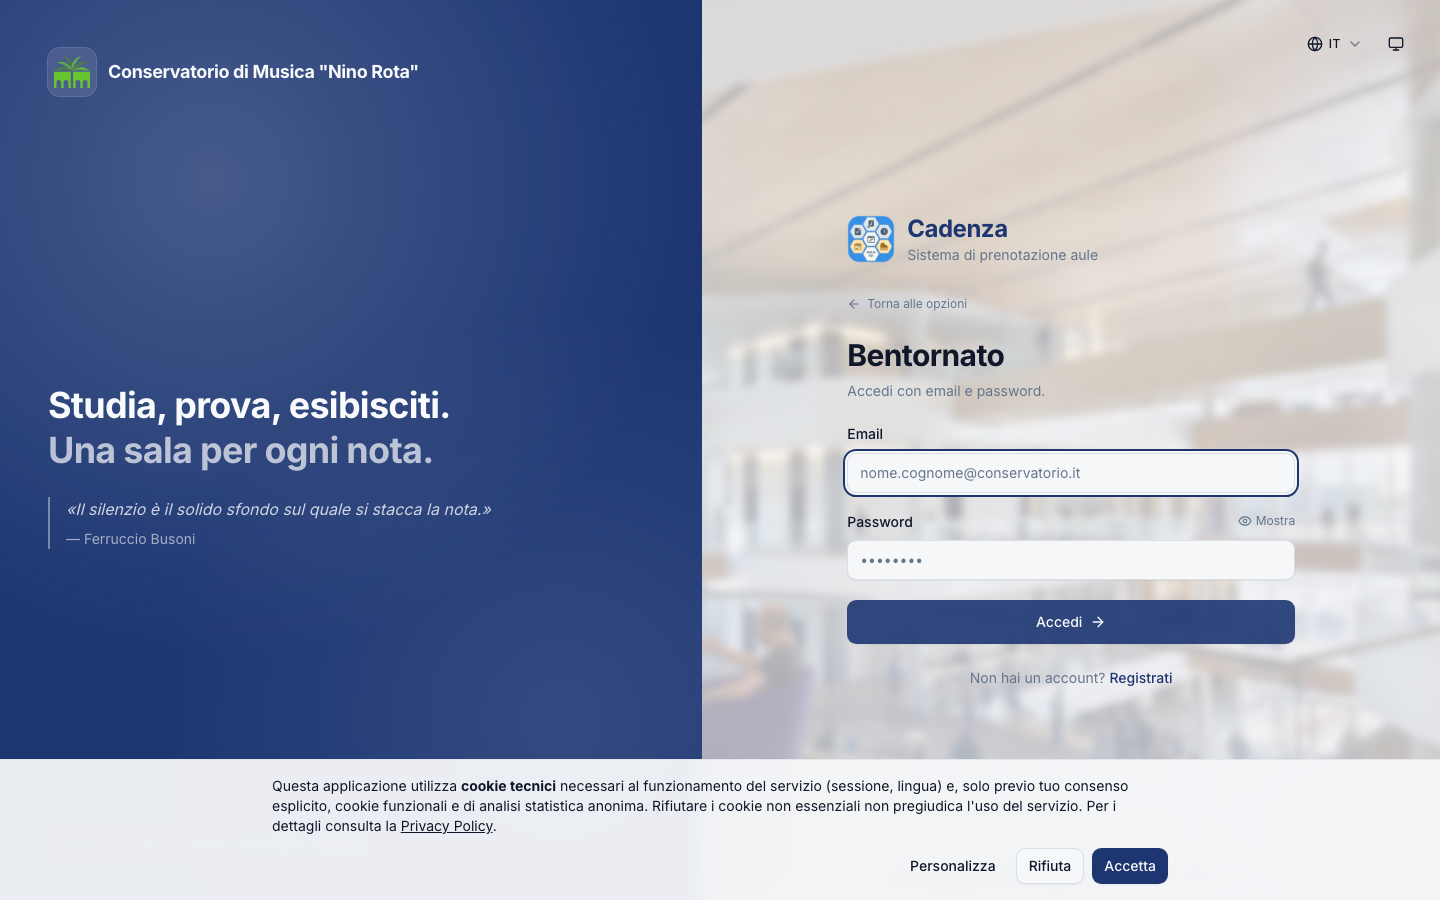
\includegraphics[width=0.95\linewidth]{screenshots/login-email.png}\caption*{Schermata di login con il form email + password aperto}\end{figure}

\begin{quote}
\textbf{Primo accesso?} Dopo aver creato l'account, la pagina ti chiede di completare il profilo (matricola, corso, ecc.) prima di poter usare il sistema.
\end{quote}

\begin{figure}[H]\centering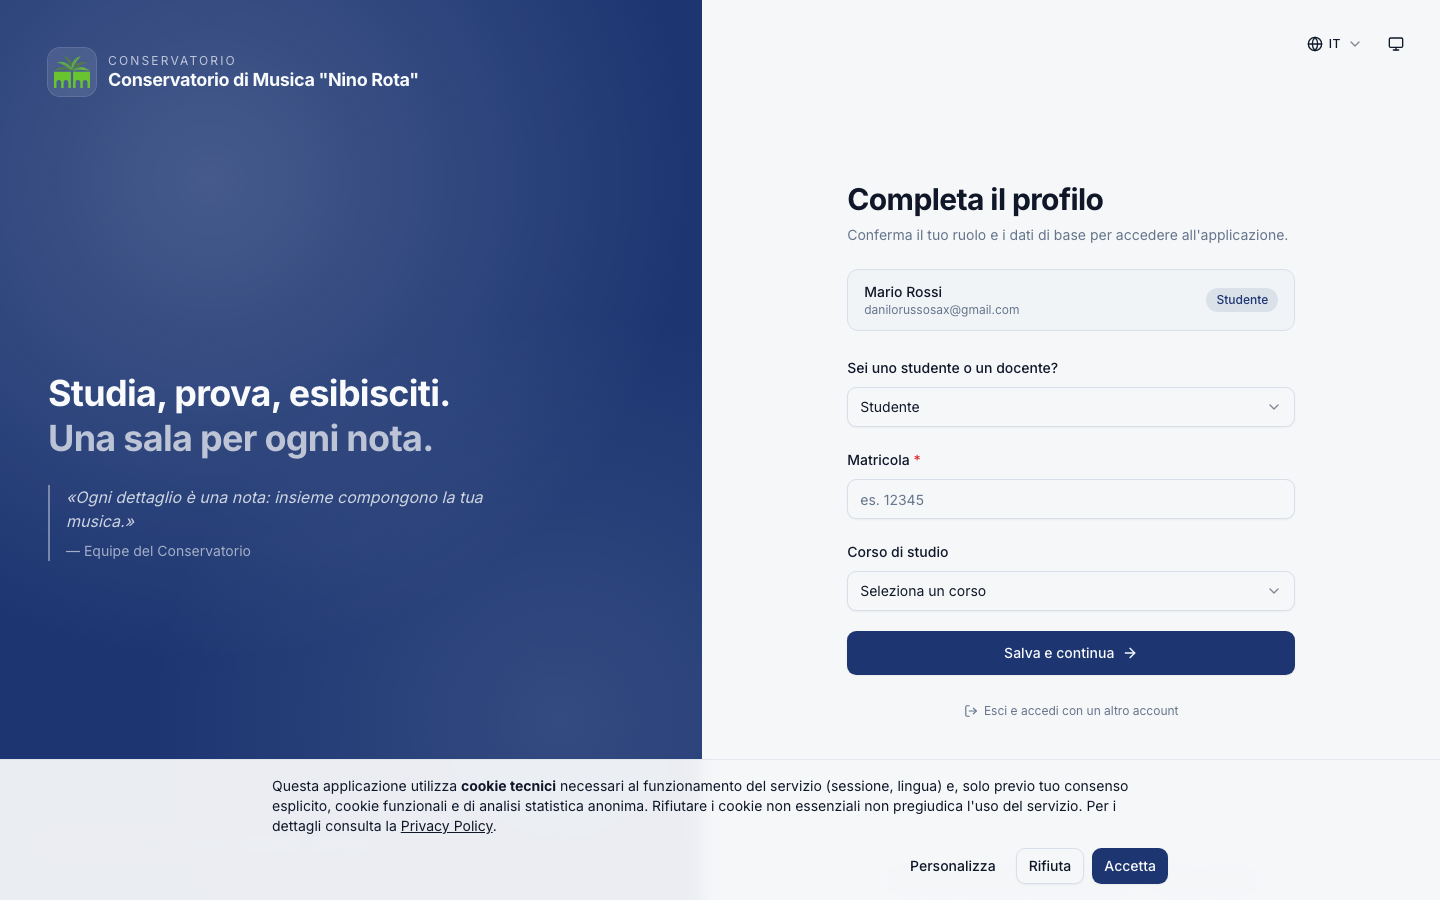
\includegraphics[width=0.95\linewidth]{screenshots/complete-profile.png}\caption*{Pagina di completamento profilo al primo accesso}\end{figure}

\subsection{2.2 Sidebar Amministrazione}


Una volta loggato come admin, la sidebar a sinistra mostra in basso la sezione \textbf{"AMMINISTRAZIONE"} con queste voci:

\begin{lstlisting}
AMMINISTRAZIONE
├─ Utenti                   <- §3
├─ Corsi                    <- §4
├─ Gestione Monte Ore       <- §8
├─ Regole prenotazioni      <- §6
├─ Approvazioni             <- §7.1   (badge se ci sono richieste in sospeso)
├─ Registro attività        <- §7.2   (cancellazioni in blocco + scambio aula)
├─ Struttura                <- §5
├─ Inventario strumenti     <- §9
├─ Statistiche              <- §10
├─ Annunci                  <- §11
└─ Impostazioni Server      <- §12
\end{lstlisting}

Le voci \textbf{Monte Ore} e \textbf{Inventario strumenti} sono nascondibili da \textit{Impostazioni Server → Moduli} se il Conservatorio non li usa (vedi §12.9).

\subsection{2.3 Dashboard utente}


La dashboard è la \textbf{prima pagina} che vedi dopo il login. Riassume in un colpo d'occhio: prossime prenotazioni, calendario aule, eventuali notifiche.

\begin{figure}[H]\centering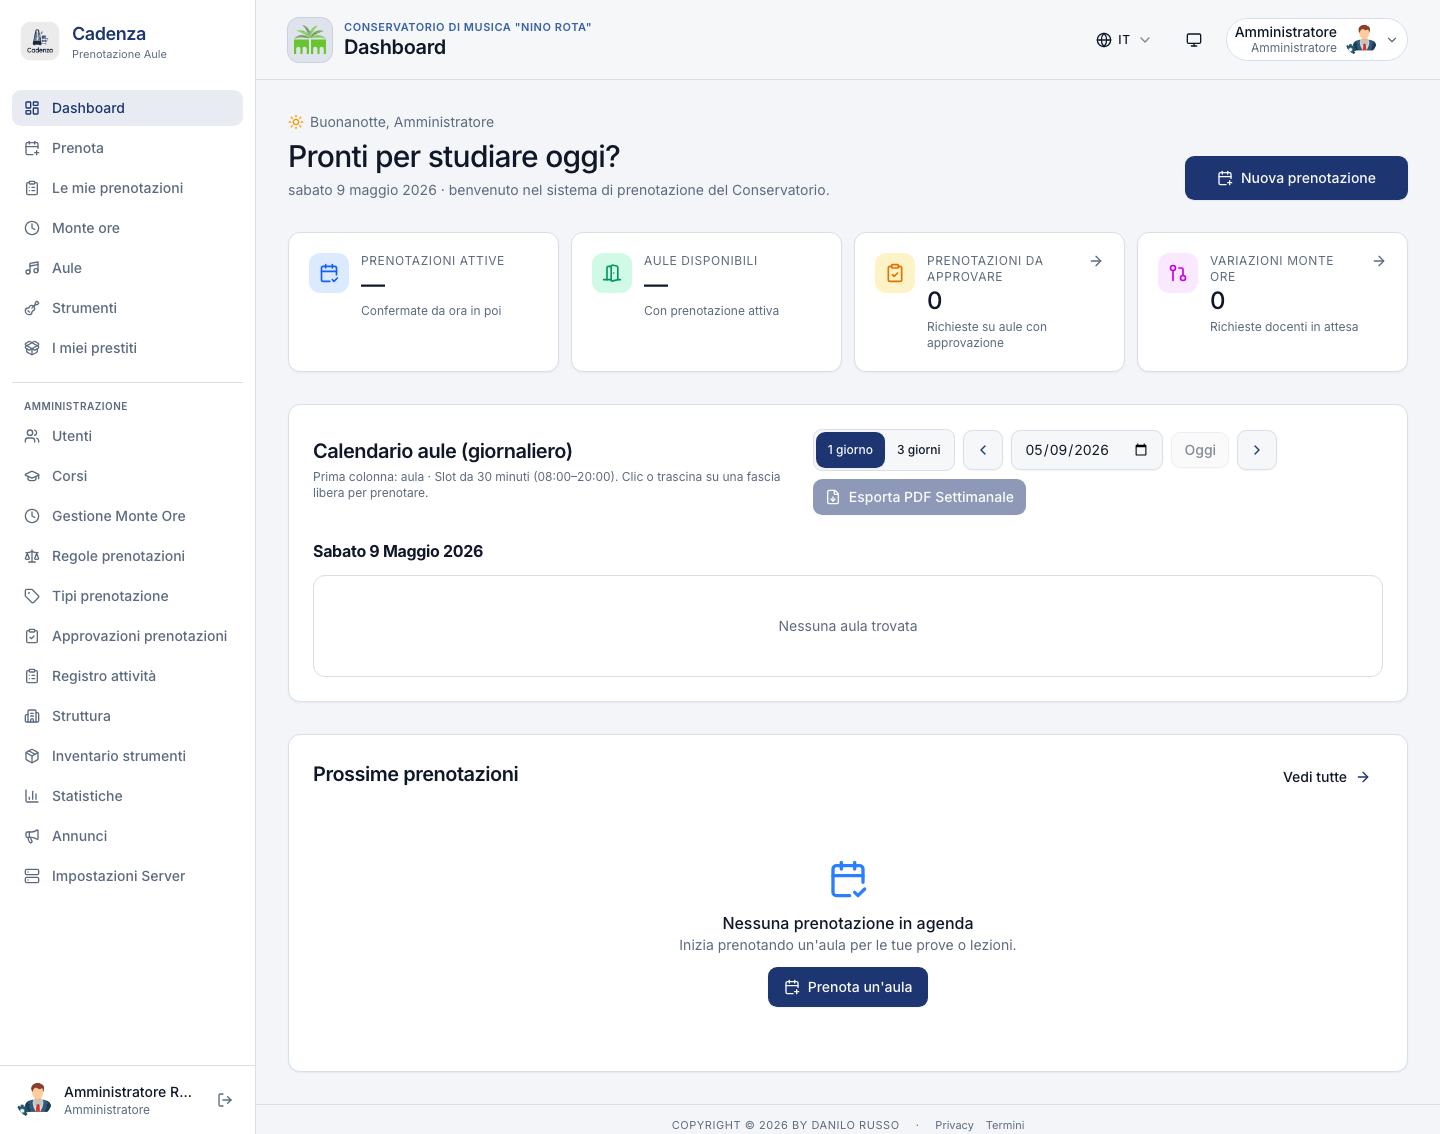
\includegraphics[width=0.95\linewidth]{screenshots/dashboard-overview.png}\caption*{Dashboard utente — vista 1 giorno (default)}\end{figure}

\subsection{2.4 Vista del calendario in dashboard (1 / 3 giorni)}


Sulla dashboard la card del calendario ha un toggle in alto a destra: \textbf{\texttt{1 giorno · 3 giorni}}. Quando è attiva la modalità "3 giorni" vedi affiancati il giorno corrente e i due successivi. La preferenza viene ricordata sul tuo browser, e le frecce di navigazione avanzano in passi coerenti (1 oppure 3 giorni).

\begin{figure}[H]\centering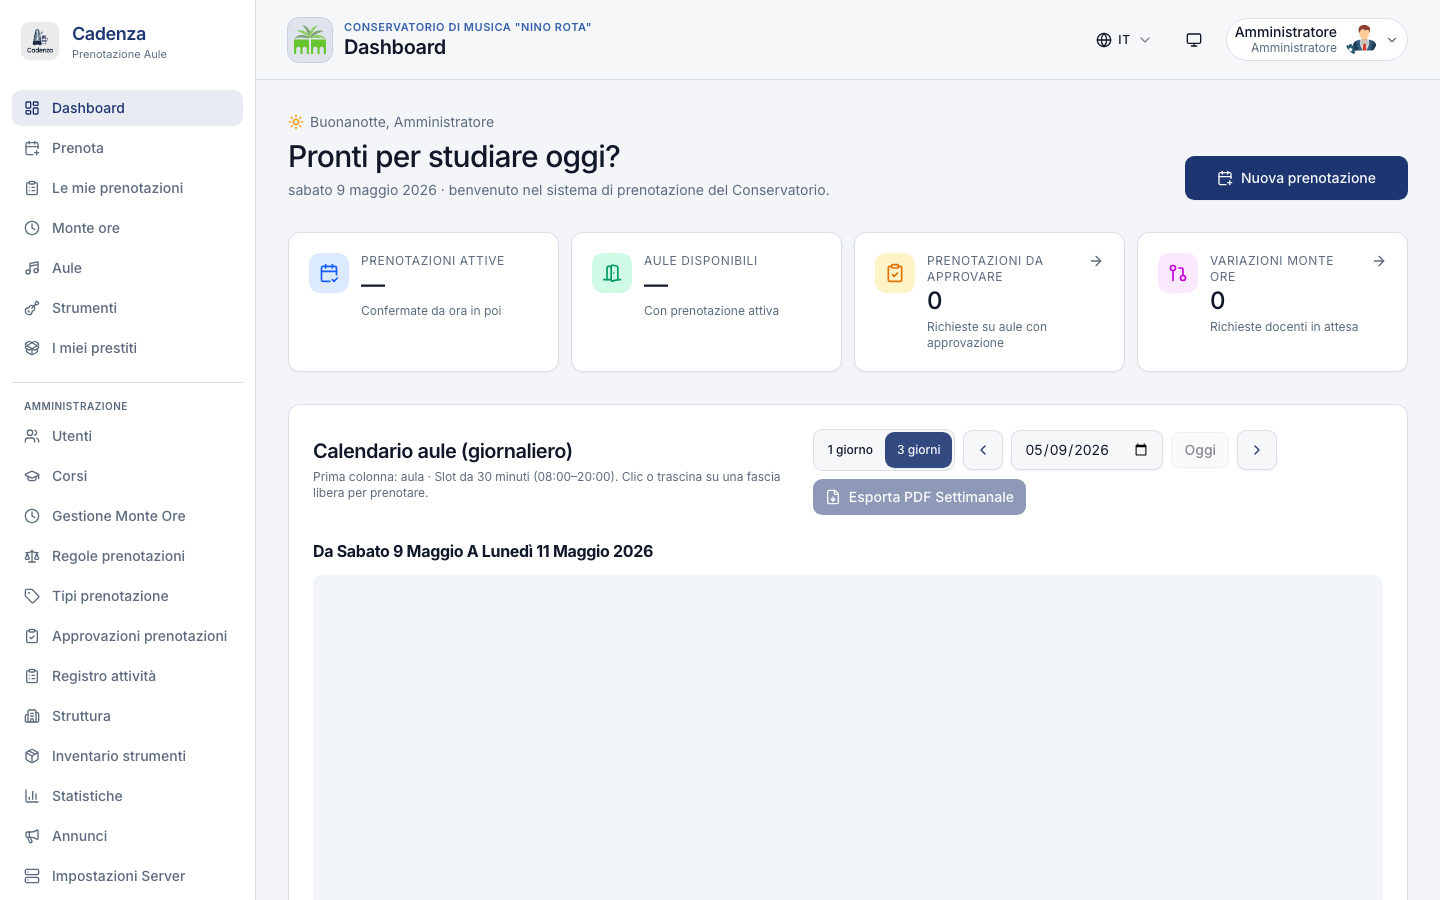
\includegraphics[width=0.95\linewidth]{screenshots/dashboard-calendario-3giorni.png}\caption*{Dashboard — vista calendario "3 giorni" affiancati}\end{figure}

\subsection{2.5 Pagine principali per l'utente}


Tutti gli utenti (studente / docente / admin) hanno accesso alle stesse pagine "operative". L'admin in più ha la sezione AMMINISTRAZIONE descritta sopra.

\begin{itemize}
  \item \textbf{Prenota} (\texttt{/booking}) --- cerchi l'aula, scegli giorno e orario, prenoti. \begin{figure}[H]\centering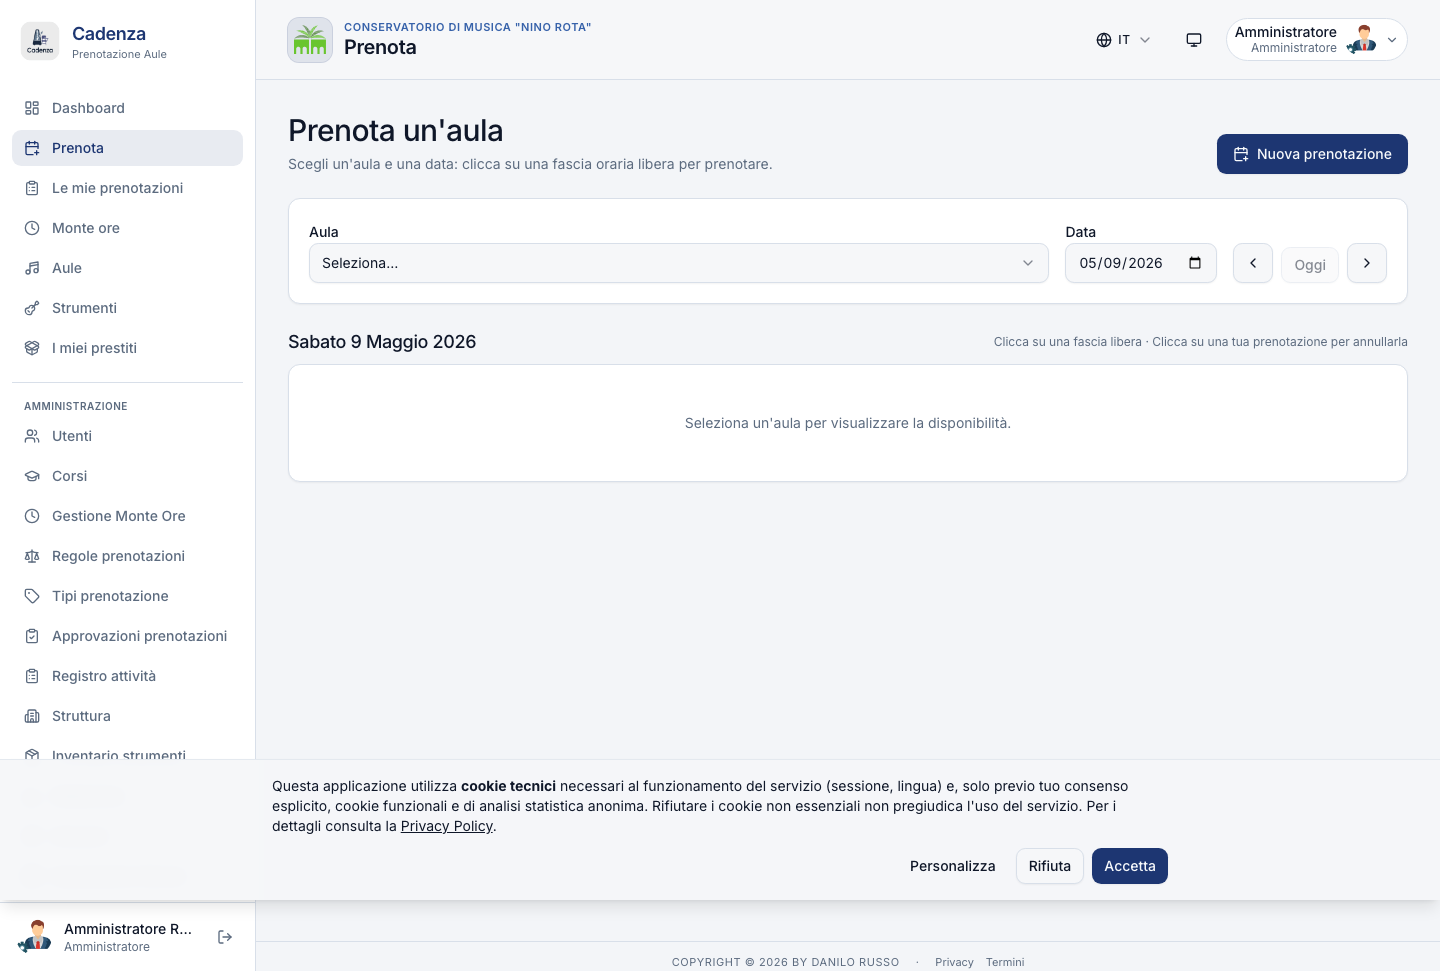
\includegraphics[width=0.95\linewidth]{screenshots/booking-page.png}\caption*{Pagina di prenotazione — selezione aula + slot 30 min}\end{figure}
  \item \textbf{Le mie prenotazioni} (\texttt{/my-bookings}) --- riepilogo con tab future / passate / annullate. \begin{figure}[H]\centering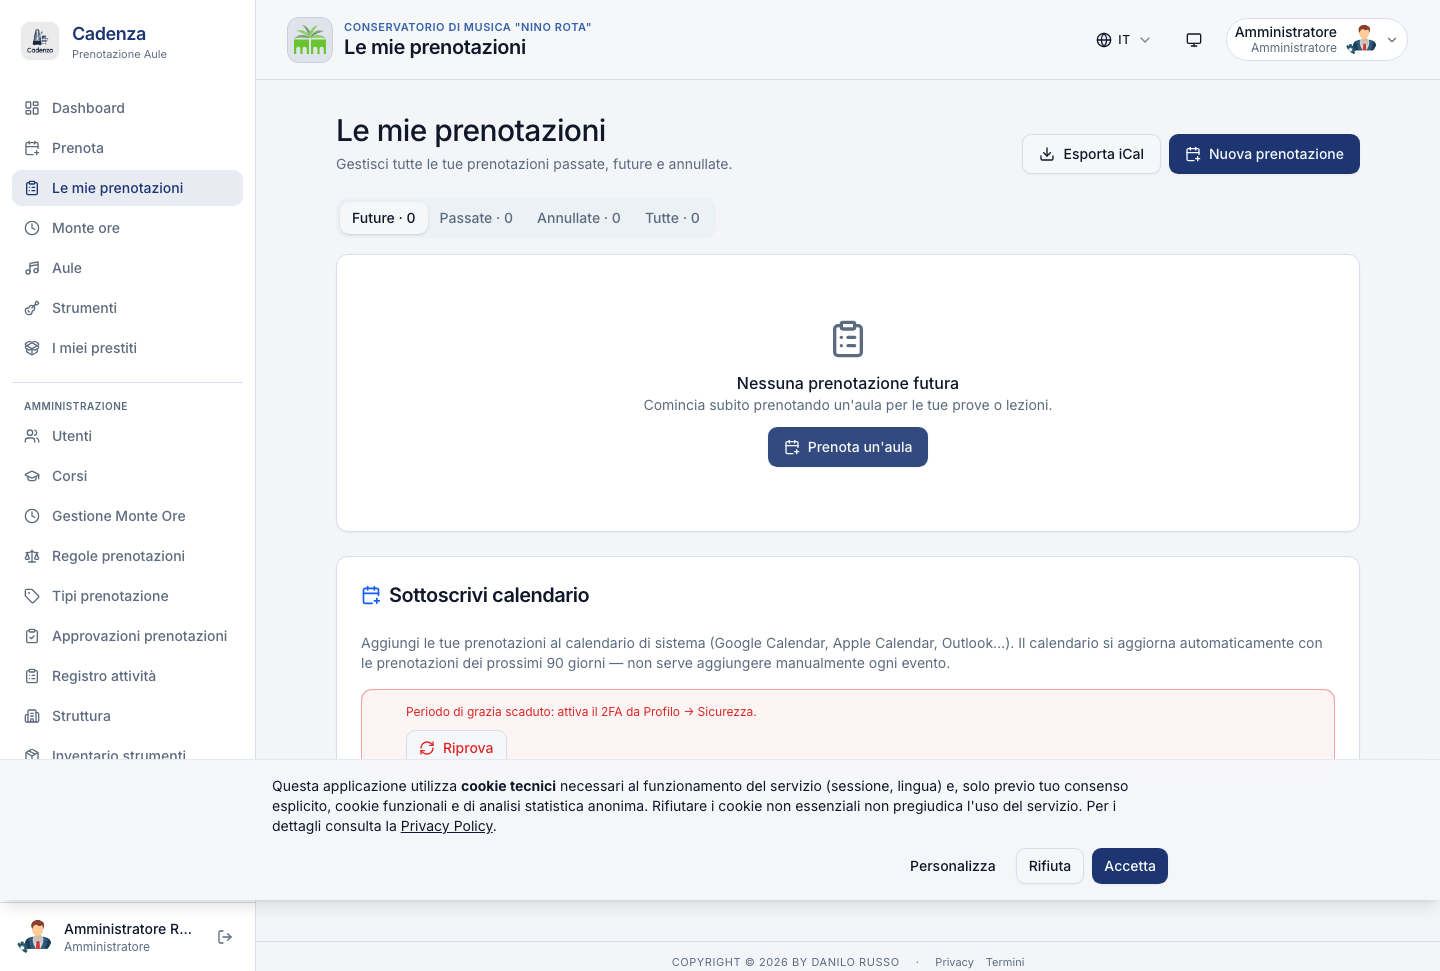
\includegraphics[width=0.95\linewidth]{screenshots/my-bookings.png}\caption*{Le mie prenotazioni — tab future, passate, annullate}\end{figure}
  \item \textbf{Aule} (\texttt{/rooms}) --- directory raggruppata per edificio con foto e dotazioni. \begin{figure}[H]\centering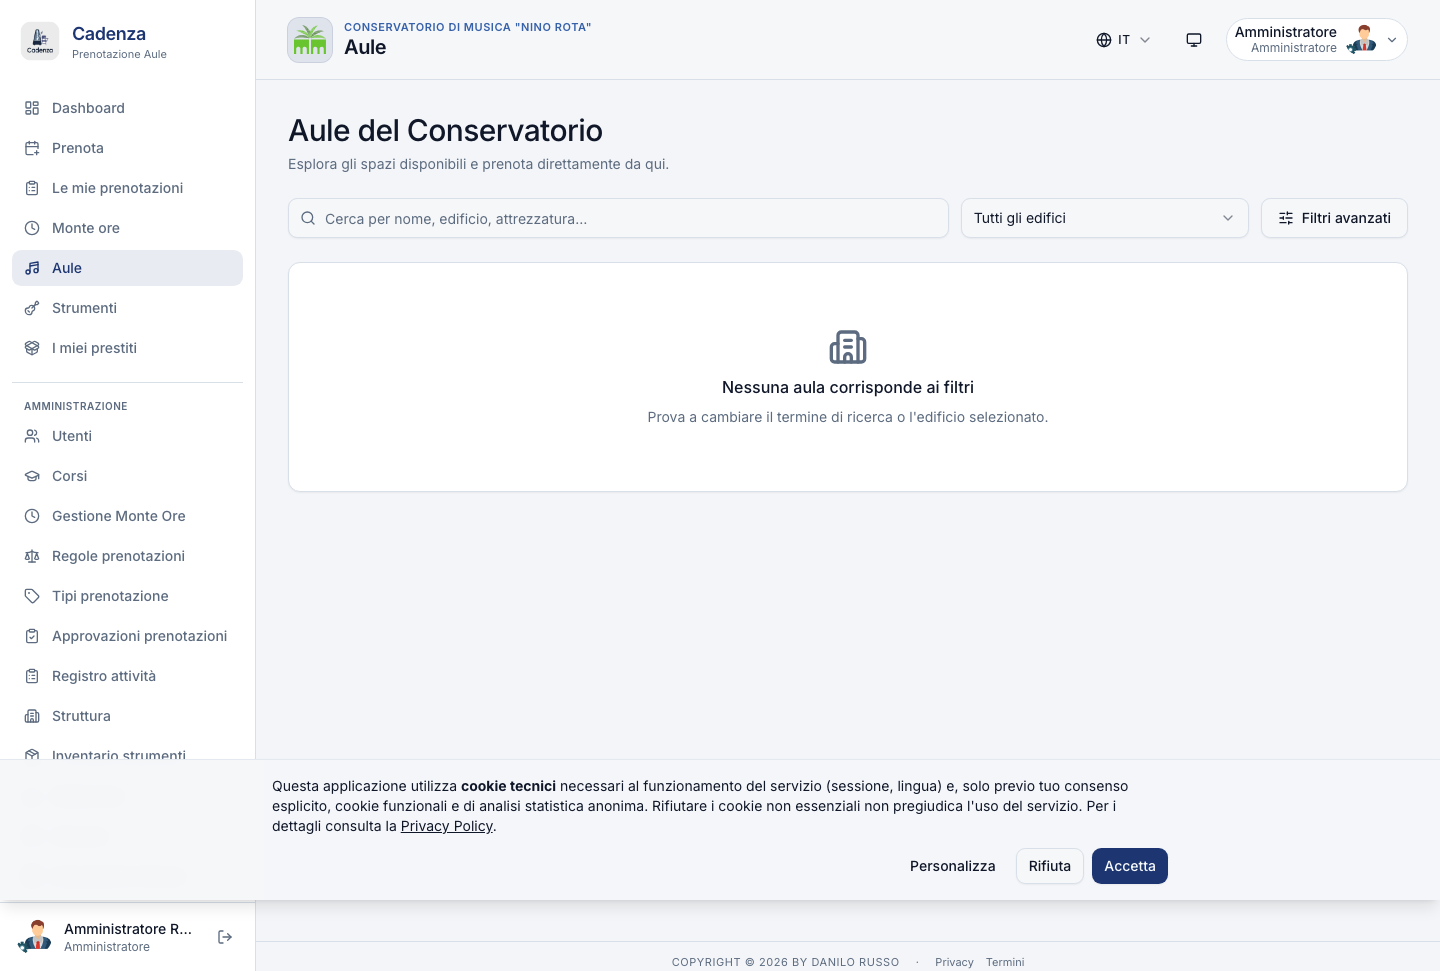
\includegraphics[width=0.95\linewidth]{screenshots/rooms-grouped.png}\caption*{Pagina Aule — sezioni espandibili per edificio}\end{figure}
  \item \textbf{Profilo} (\texttt{/profile}) --- anagrafica, password, preferenze notifiche, link iCal personale. \begin{figure}[H]\centering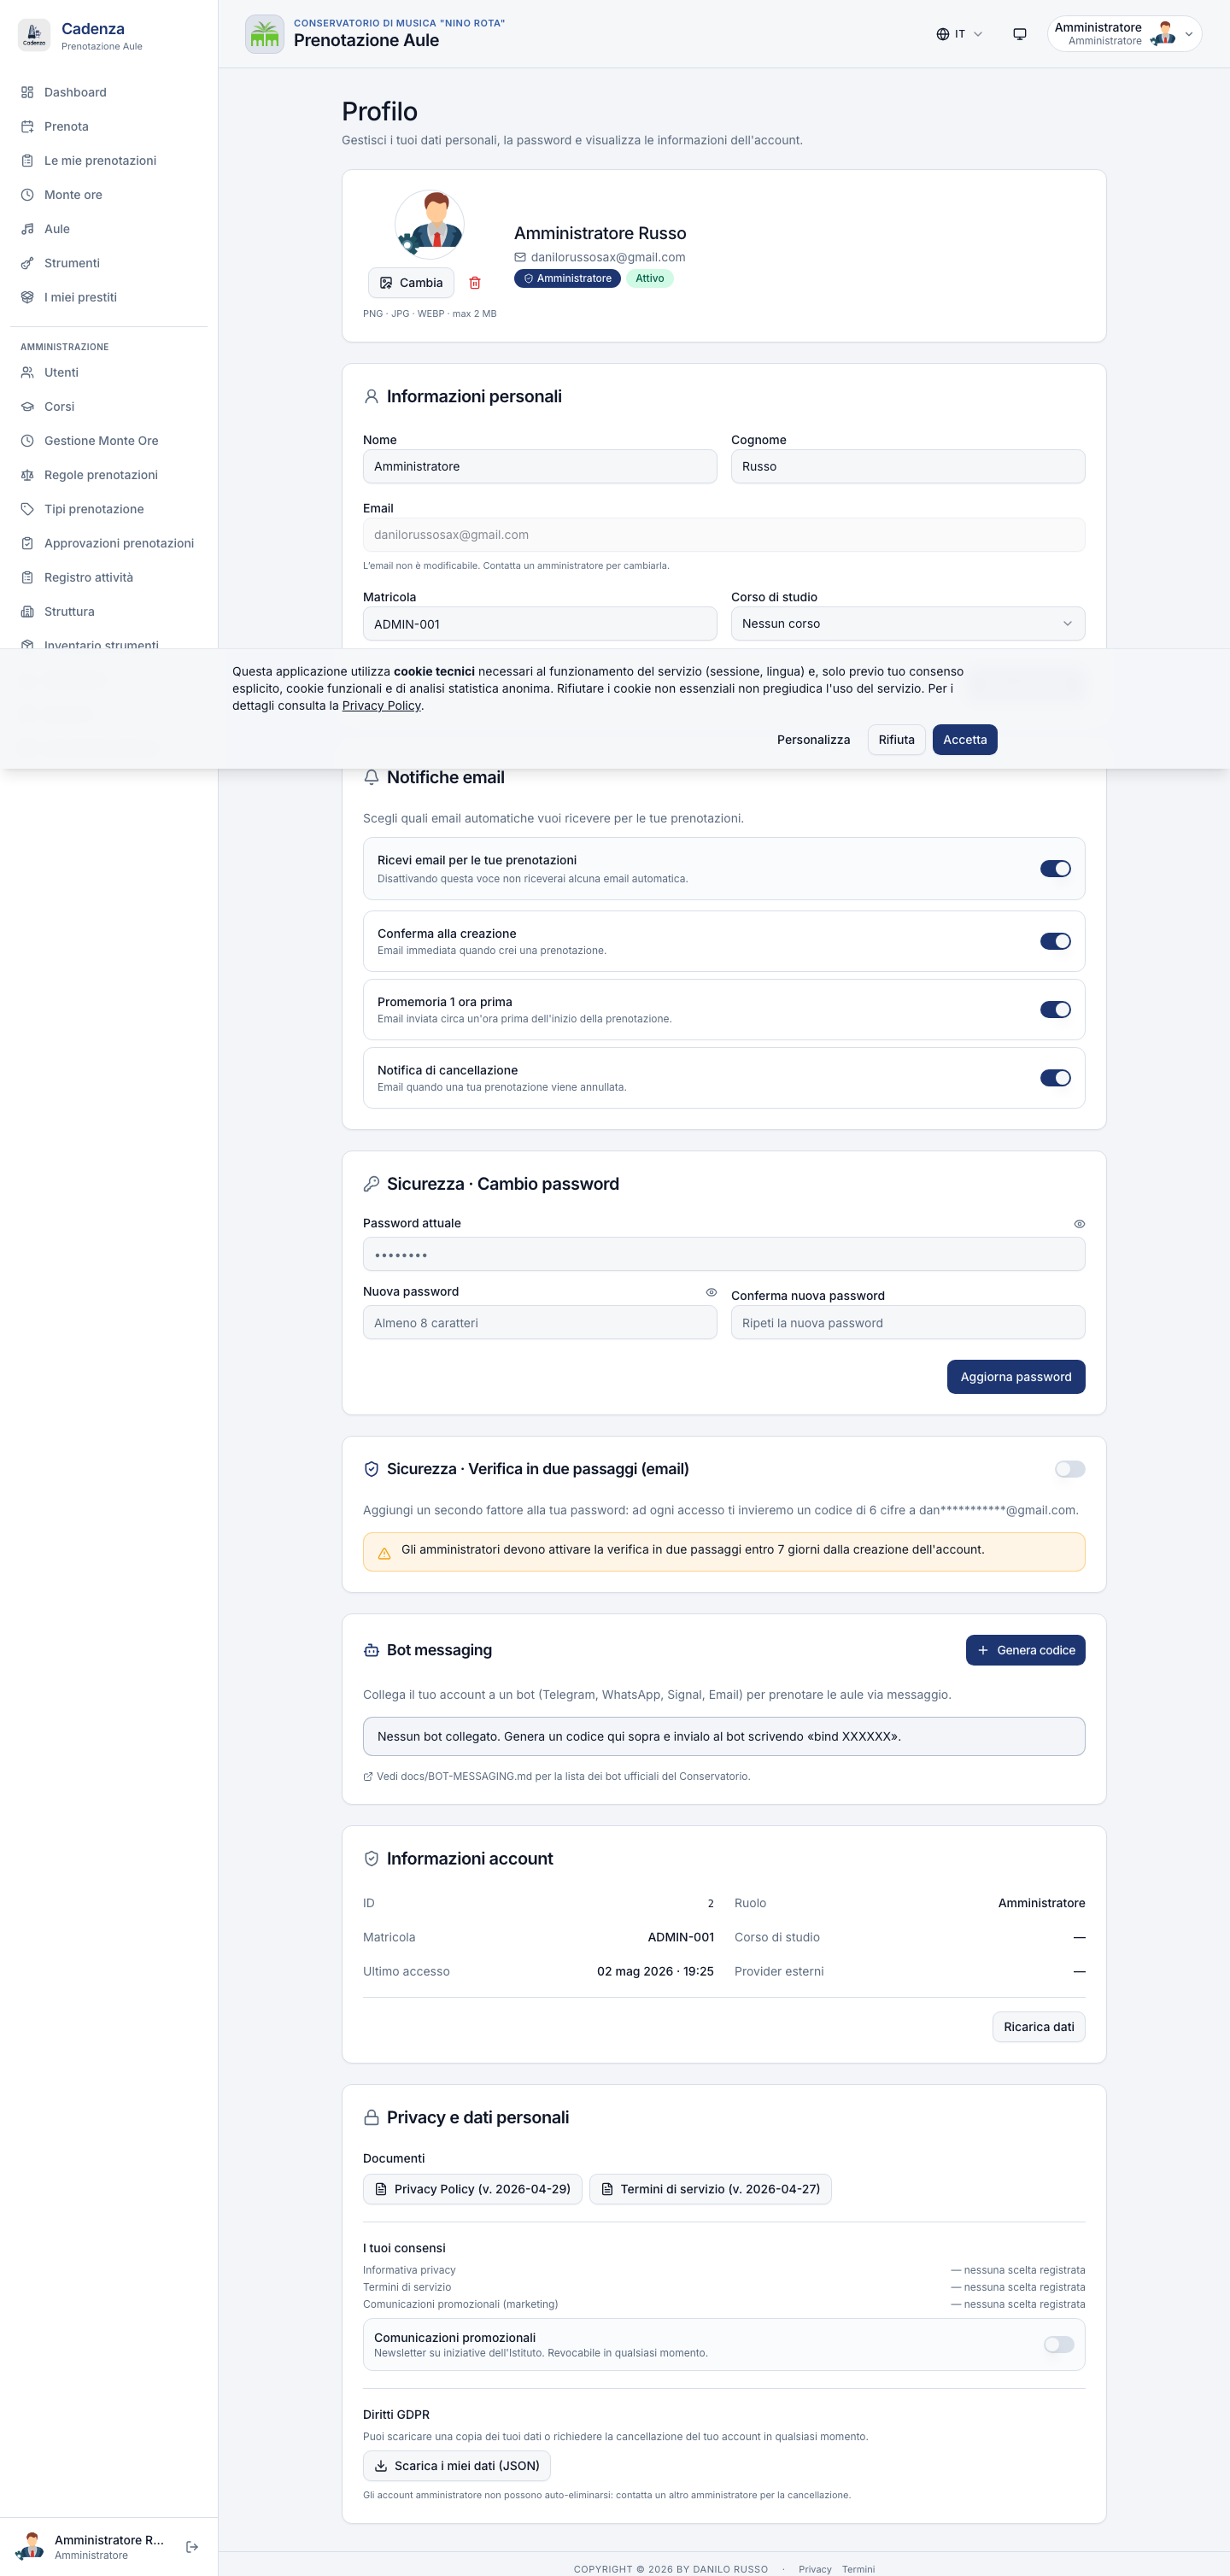
\includegraphics[width=0.95\linewidth]{screenshots/profile-page.png}\caption*{Pagina Profilo — anagrafica e preferenze}\end{figure} \begin{figure}[H]\centering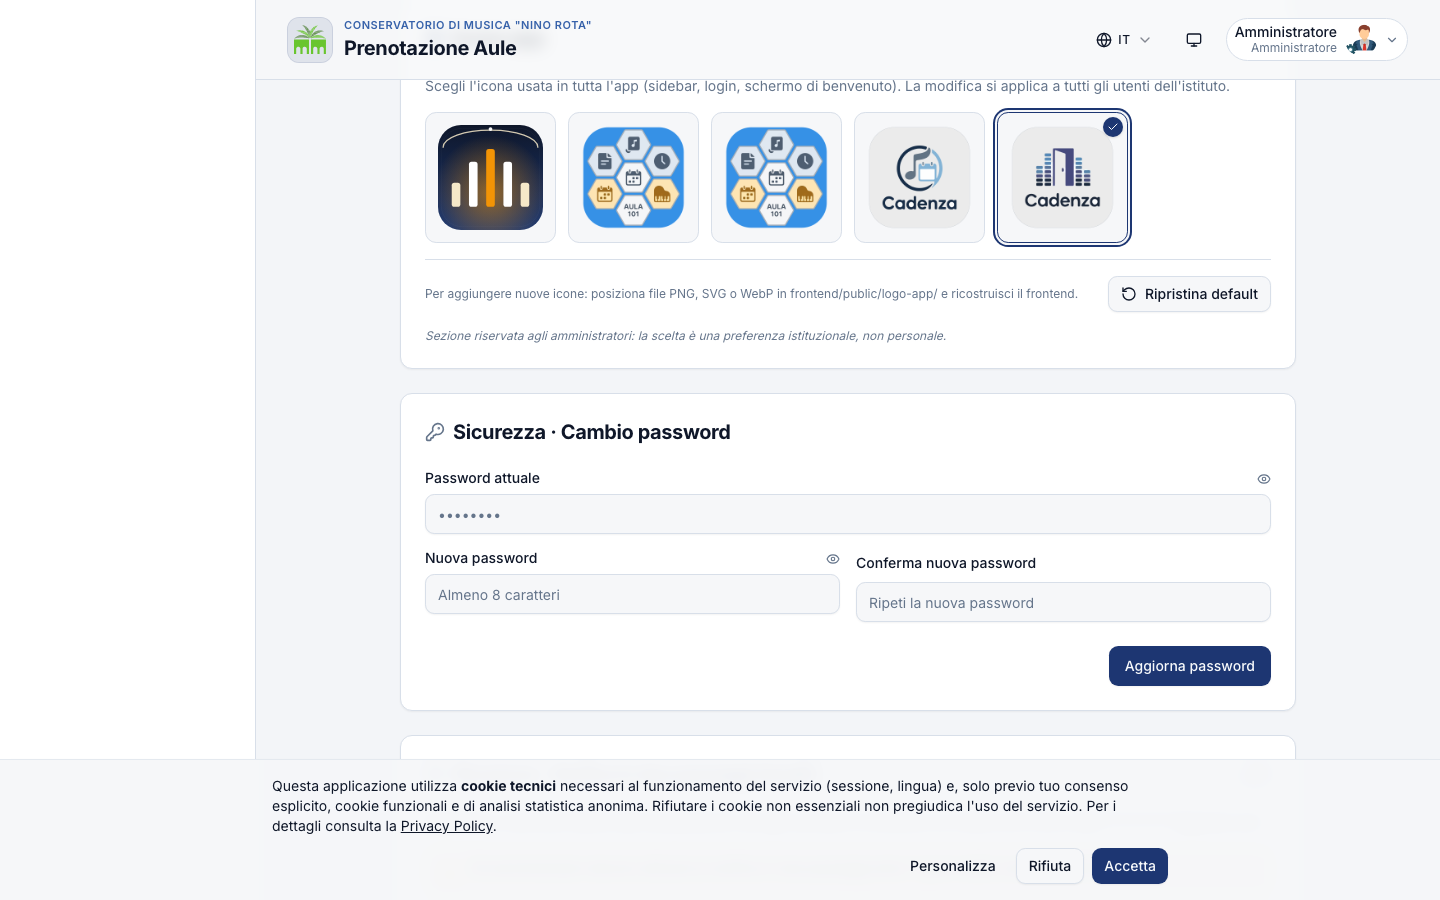
\includegraphics[width=0.95\linewidth]{screenshots/profile-app-icon.png}\caption*{Pagina Profilo — card "Aggiungi a Home" (PWA, icona dell'app)}\end{figure}
\end{itemize}

\begin{quote}
\textbf{Differenza tra "Sidebar Operazioni" e "Impostazioni Server"}: le prime 11 voci della sidebar sono per le \textbf{attività quotidiane}. \textit{Impostazioni Server} raggruppa invece la \textbf{configurazione del sistema} (mail, QR, display, audit, backup, moduli) ed è la voce che apri raramente.
\end{quote}

\medskip\hrule\medskip

\section{3. Utenti}


URL: \texttt{/admin/users}

\begin{figure}[H]\centering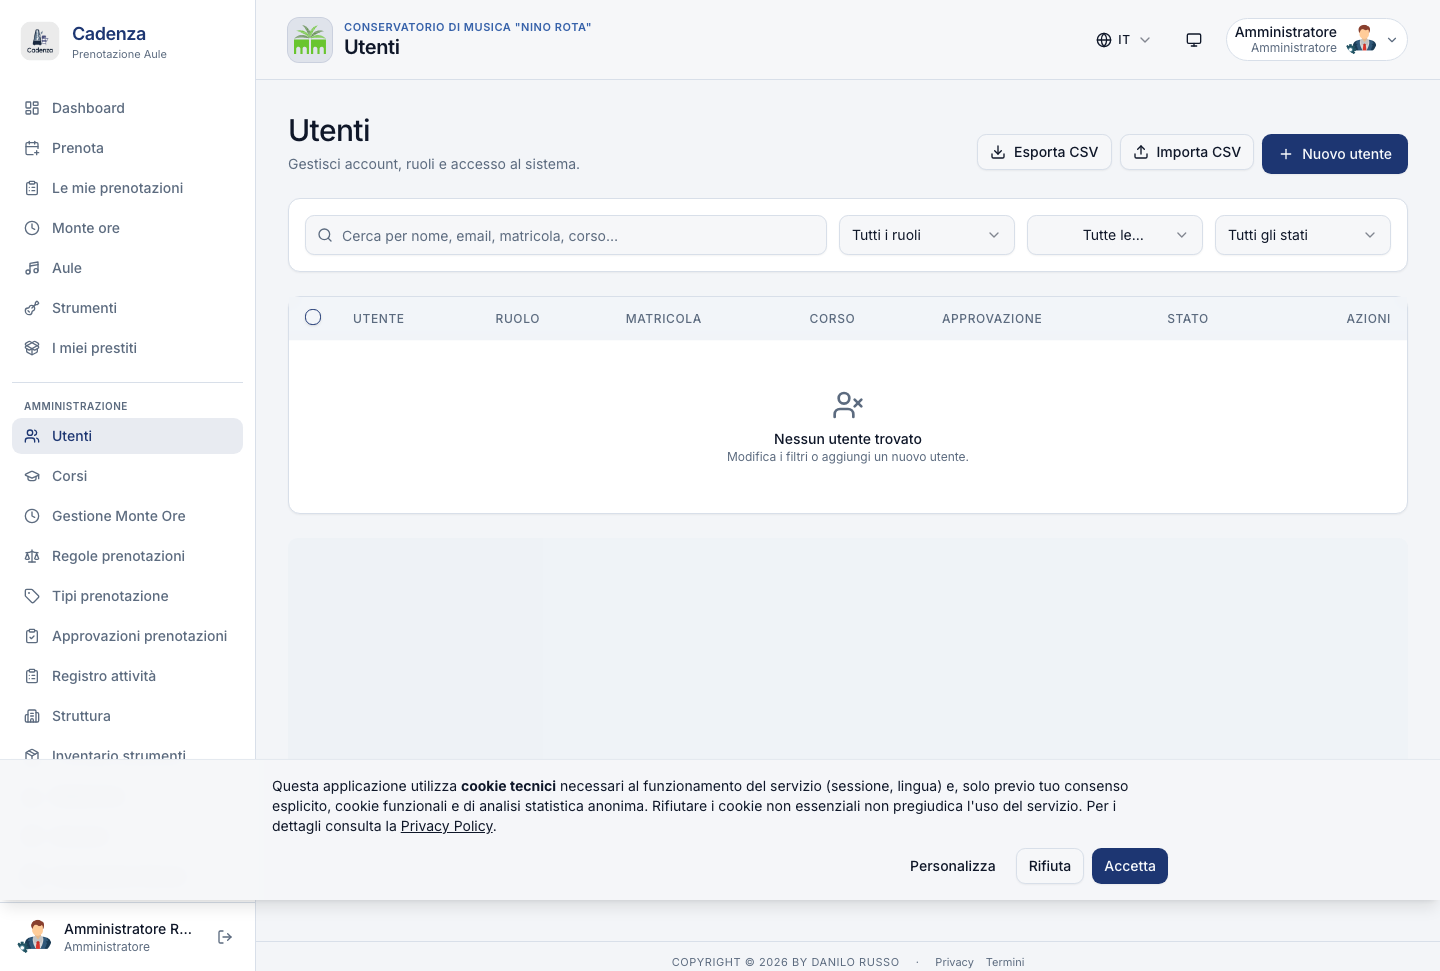
\includegraphics[width=0.95\linewidth]{screenshots/users-overview.png}\caption*{Pagina Utenti — toolbar, filtri, tabella e barra azioni in blocco}\end{figure}

\subsection{3.1 Cosa puoi fare in questa pagina}


\begin{itemize}
  \item Vedere e cercare tutti gli utenti del Conservatorio.
  \item Approvare o rifiutare nuove registrazioni.
  \item Modificare anagrafica e ruolo di un utente esistente.
  \item Disattivare o cancellare account.
  \item Operare in blocco su più utenti contemporaneamente.
  \item Configurare l'accesso con Google e Microsoft (sotto la tabella).
  \item Importare le anagrafiche da Isidata (card "Integrazione anagrafiche").
\end{itemize}

\subsection{3.2 Toolbar e filtri}


In testa alla pagina trovi:

\begin{itemize}
  \item \textbf{Ricerca testuale}: cerca su nome, cognome, email, matricola e corso.
  \item \textbf{Filtro Ruolo}: tutti / Admin / Docente / Studente.
  \item \textbf{Filtro Approvazione}: tutti / In attesa / Approvati / Rifiutati.
  \item \textbf{Filtro Stato account}: tutti / Attivi / Disattivati.
\end{itemize}

I filtri sono immediati: scrivi e la lista si aggiorna senza ricaricare la pagina.

\subsection{3.3 Tabella utenti}


Le colonne mostrano: avatar + nome, email, ruolo (badge), matricola, corso, stato di approvazione, account attivo/disattivato, e le azioni (\checkmark{} approva, \texttimes{} rifiuta, \textit{mod.} modifica, \textit{canc.} elimina). Sulla tua riga personale alcune azioni sono disabilitate per evitare di disattivarti o eliminarti per sbaglio.

\subsection{3.4 Bulk action bar (azioni in blocco)}


Selezionando una o più righe (checkbox a sinistra) compare in alto una barra giallo-ambra con i bottoni:

\begin{itemize}
  \item \textbf{Pulisci} --- annulla la selezione
  \item \textbf{Approva} / \textbf{Rifiuta} --- su tutti i selezionati
  \item \textbf{Elimina} --- chiede conferma e rimuove anche le prenotazioni associate
\end{itemize}

Al termine compare un riepilogo: "N approvati, M saltati" o equivalente.

\subsection{3.5 Form Utente}


Si apre con \textbf{+ Nuovo utente} o cliccando l'icona \textit{mod.} su una riga.

Campi essenziali:

\begin{table}[H]
\centering
\small
\begin{tabularx}{\linewidth}{|X|X|}
\hline
\rowcolor{tableheader} Campo & Descrizione \\
\hline
Nome / Cognome & Dati anagrafici di base \\
\hline
Email & Sarà anche l'username per l'accesso \\
\hline
Ruolo & Admin · Docente · Studente \\
\hline
Matricola & Numero matricola istituzionale (facoltativo) \\
\hline
Corso di studio & Scelta dal catalogo dei corsi (facoltativo per docenti/admin) \\
\hline
Password & In creazione è obbligatoria; in modifica lasciala \textbf{vuota} se non vuoi cambiarla \\
\hline
Account attivo & Spegnendolo, l'utente non può più fare login senza essere cancellato \\
\hline
\end{tabularx}
\end{table}


\textbf{Sezione Monte Ore --- visibile solo per i docenti} (vedi §3.7 e §8.10):

\begin{itemize}
  \item \textbf{Tipo contratto}: titolare, supplente, contratto orario, ecc.
  \item \textbf{Override Monte Ore individuale} (interruttore) --- abilita i campi sottostanti
  \item \textbf{Ore annue}: la soglia personalizzata (es. 60h)
  \item \textbf{Esente vincolo 2-4 giorni/sett.}: per docenti che concentrano la didattica in pochi giorni
  \item \textbf{Motivazione}: testo obbligatorio quando l'override è attivo (es. "Contratto orario 60h, prot. 2026/123 del 15/09/2026")
\end{itemize}

\subsection{Banner sul form utente}


\begin{itemize}
  \item \textbf{Email rimbalzata} (giallo): se l'utente ha un indirizzo email che ha rimbalzato definitivamente, compare un alert "Email rimbalzata --- notifiche disattivate" + bottone \textbf{Riattiva} una volta corretto il problema.
  \item \textbf{Errore di salvataggio} (rosso): mostra il messaggio specifico restituito dal sistema.
\end{itemize}

\subsection{3.6 Provider OAuth (Google · Microsoft)}


In coda alla pagina Utenti due card affiancate permettono di abilitare il \textbf{login con Google Workspace} e \textbf{Microsoft 365 / Entra ID}.

\begin{figure}[H]\centering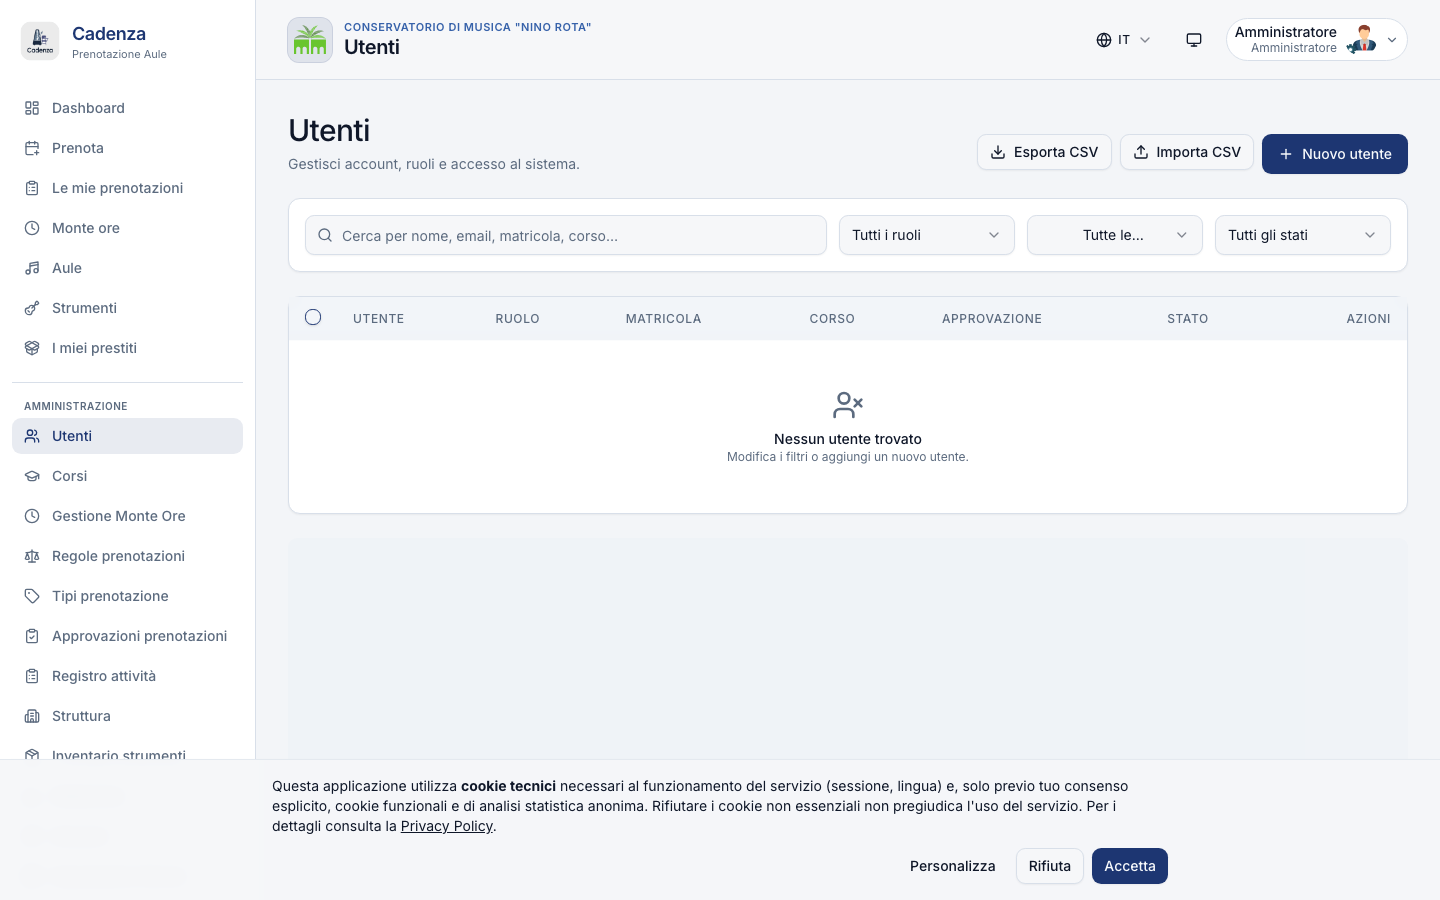
\includegraphics[width=0.95\linewidth]{screenshots/users-oauth-providers.png}\caption*{Card Provider OAuth — campi Client ID / Secret / Tenant per Google e Microsoft}\end{figure}

Per ciascun provider devi inserire i parametri ricevuti dal pannello sviluppatori del provider stesso (Client ID, Client Secret, eventuale Tenant per Microsoft, e il Callback URL). Le credenziali vengono salvate \textbf{cifrate}: nessuno, neppure l'admin, le vede in chiaro dopo il primo salvataggio.

\begin{quote}
\textbf{Importante}: dopo aver attivato un provider, \textbf{riavvia il backend} (vedi §12.4) perché il provider sia effettivamente disponibile sul login. Cadenza ti mostra un alert informativo dopo il salvataggio.
\end{quote}

Per la procedura passo-passo (creazione applicazione, configurazione redirect URI, ecc.) vedi \texttt{docs/SSO.md}.

\subsection{3.7 Deroga Monte Ore per docenti a contratto orario}


Il dettaglio della funzione è in §8.10. Qui basti sapere che dal form \textit{Modifica utente}, in coda, c'è la sezione \textbf{Monte Ore --- Tipo contratto} che permette di personalizzare la soglia annua del singolo docente. È indispensabile per i contratti orari (precari, supplenti, part-time), che hanno spesso un monte ore concordato individualmente diverso dalle 324 ore CCNL del titolare di ruolo.

\begin{figure}[H]\centering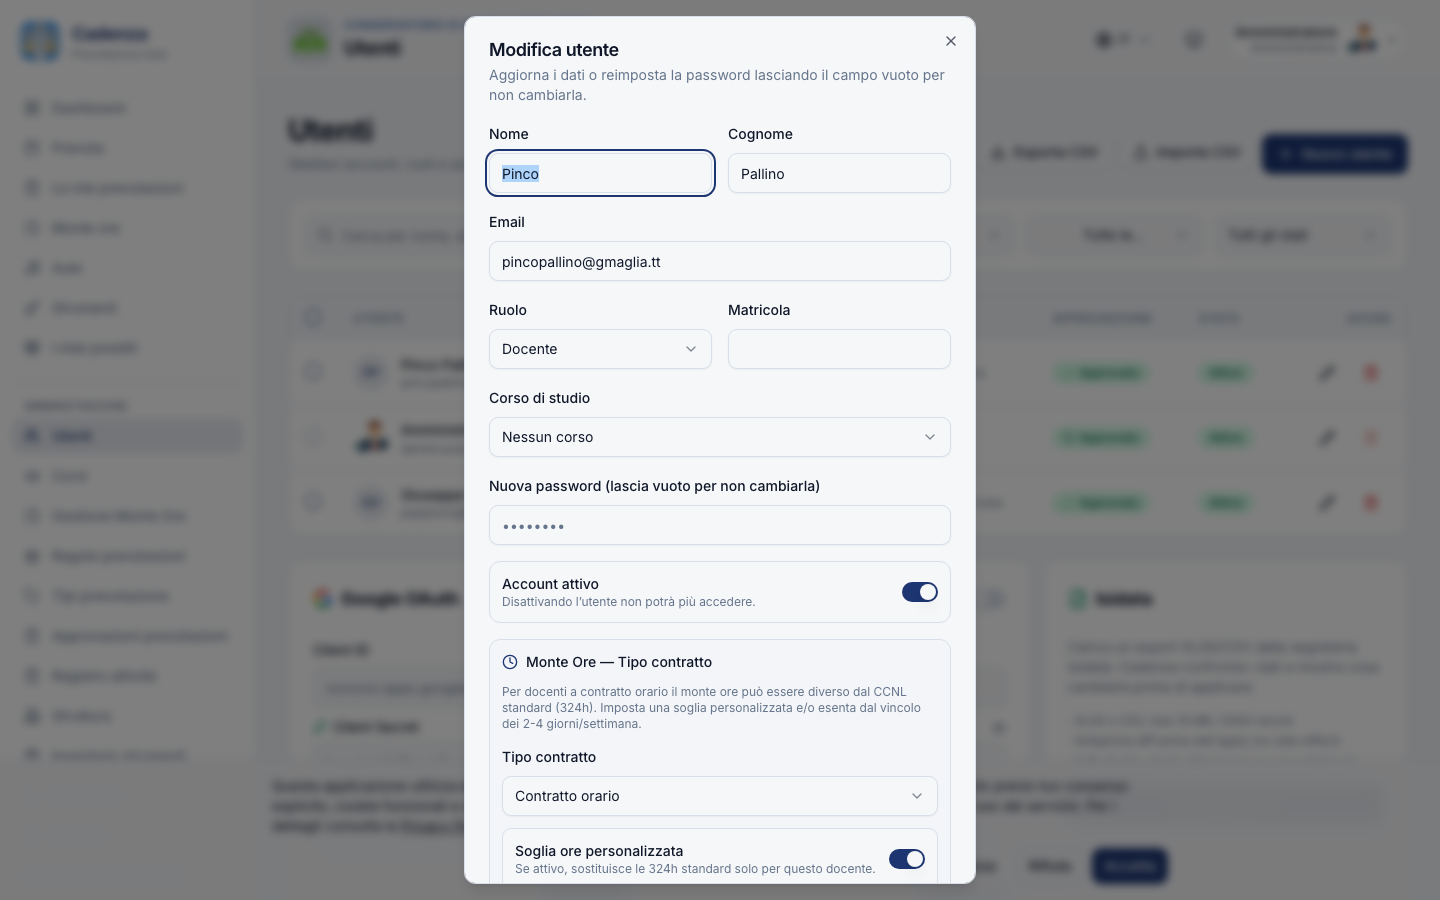
\includegraphics[width=0.95\linewidth]{screenshots/users-form-monteore-override.png}\caption*{Form deroga Monte Ore — sezione visibile solo per docenti}\end{figure}

\subsection{3.8 Politiche di password e sicurezza}


Cadenza richiede password di \textbf{almeno 10 caratteri}, con almeno una \textbf{lettera maiuscola} e almeno una \textbf{cifra}. È la policy raccomandata dalle linee guida AGID 2024 per la PA italiana. Le password storiche più corte continuano a funzionare per il login, ma alla prossima richiesta di cambio dovranno rispettare le nuove soglie.

I tentativi di login, registrazione, invio del codice di sicurezza e generazione di prenotazioni ricorrenti sono \textbf{rate-limited}: dopo un numero di tentativi falliti l'IP riceve un blocco temporaneo, per proteggere il sistema da brute-force e spam. L'utente vede un messaggio chiaro tipo "Troppi tentativi, riprova tra X secondi".

\textbf{Password reset self-service}: gli utenti che dimenticano la password non hanno più bisogno di un admin. Dalla pagina di login cliccano "Password dimenticata?", inseriscono l'email, ricevono un link valido 1 ora utilizzabile una volta sola, e impostano una nuova password. Il flusso è anti-enumeration (la stessa risposta indipendentemente dall'esistenza dell'email) e ha doppio rate-limit (per IP + per utente). Il cambio password \textbf{invalida tutte le sessioni JWT esistenti} e sblocca eventuale account lockout. Dettagli operativi nel manuale docente §2.2-bis.

\subsection{3.9 Anti-blocco amministratore}


Cadenza non ti permette di fare azioni che lascerebbero il sistema senza nessun amministratore attivo:

\begin{itemize}
  \item Non puoi auto-degradarti a docente o studente.
  \item Non puoi disattivarti o eliminarti.
  \item Non puoi cancellare l'ultimo admin attivo dell'istituto.
\end{itemize}

Per dismettere un admin servono almeno \textbf{due} admin attivi, in modo che ne resti sempre uno. Se hai bisogno di chiudere completamente il Conservatorio (cessazione), serve un intervento del personale tecnico (DBA con accesso al database).

\medskip\hrule\medskip

\section{4. Corsi e Livelli}


URL: \texttt{/admin/courses} (con scheda \texttt{?tab=corsi|livelli})

\subsection{4.1 Layout}


La pagina ha due \textbf{macro-tab} in alto:

\begin{itemize}
  \item \textbf{Corsi} (catalogo SAD del Conservatorio)
  \item \textbf{Livelli} (propedeutico, triennio, biennio, master, ecc.)
\end{itemize}

\subsection{4.2 Tab "Corsi"}


\begin{figure}[H]\centering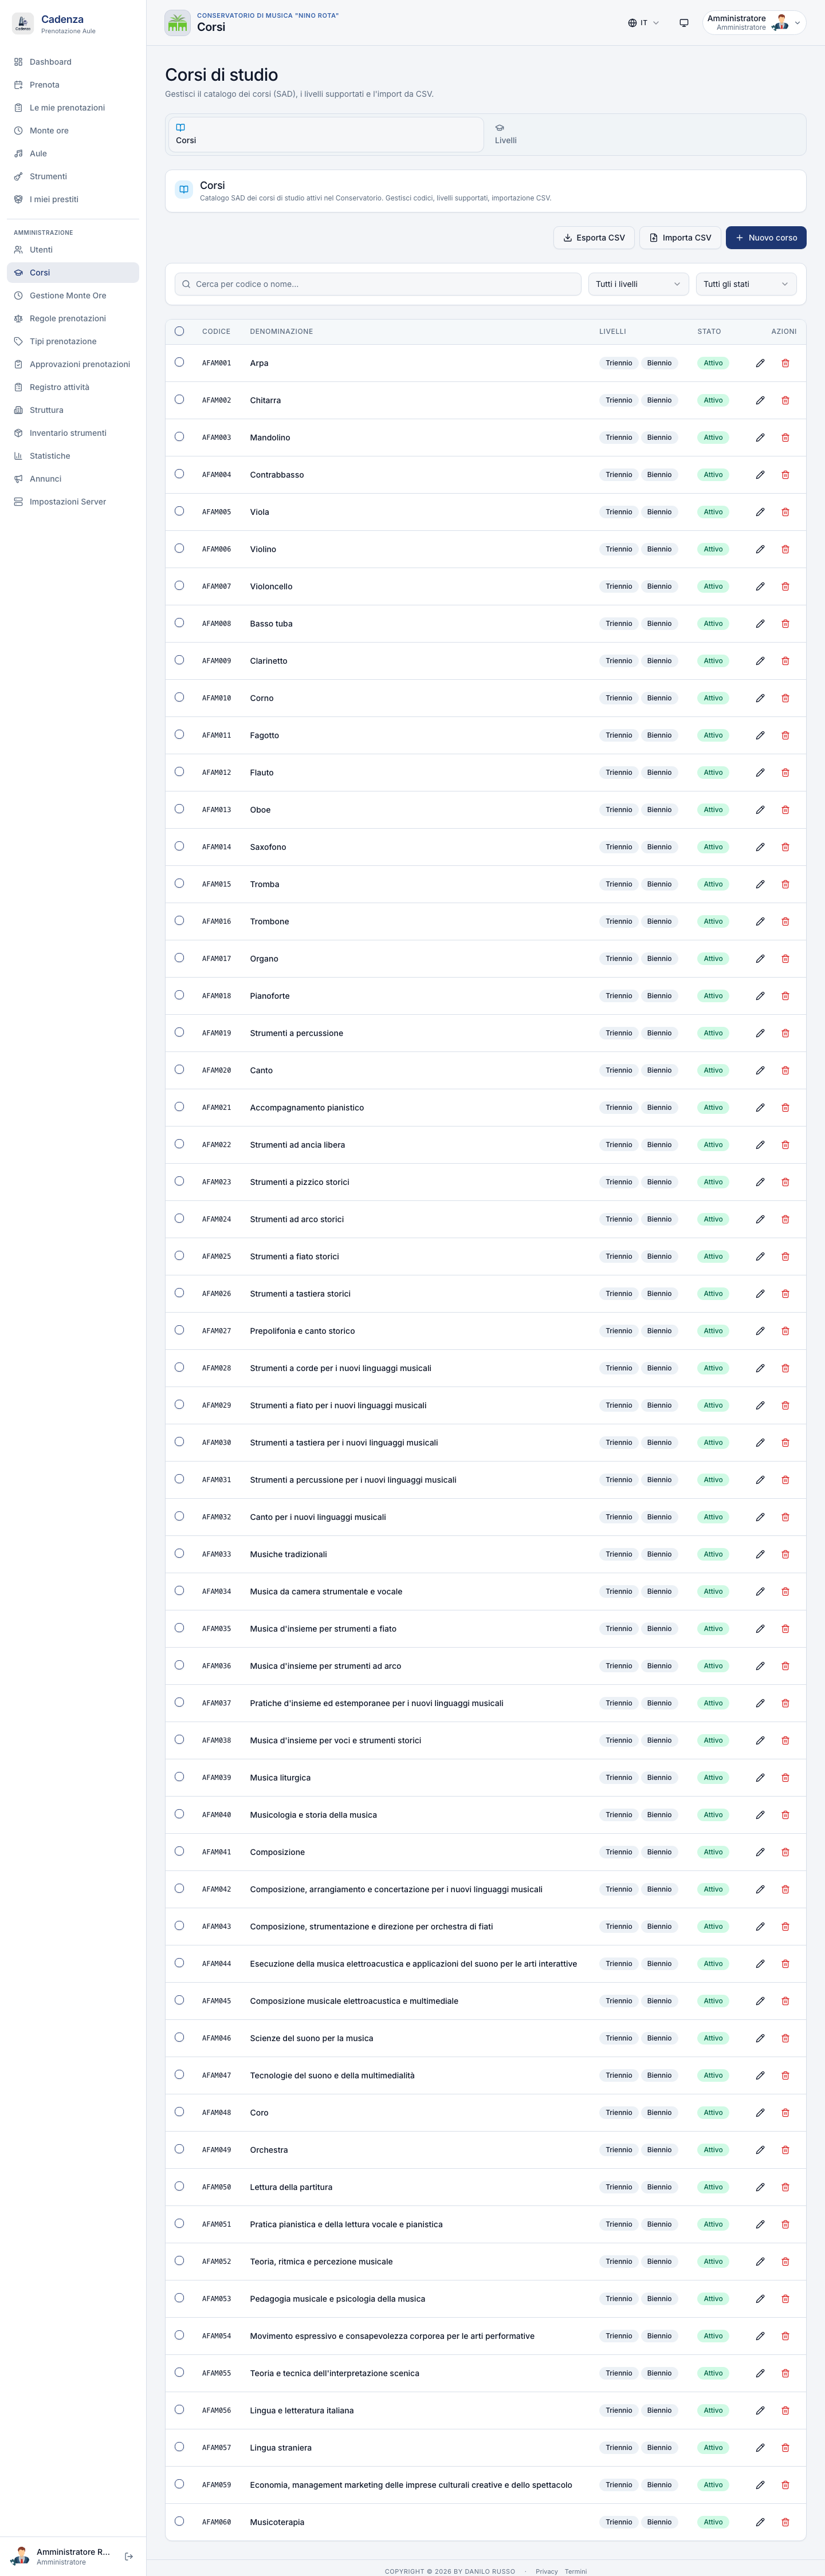
\includegraphics[width=0.95\linewidth]{screenshots/courses-overview.png}\caption*{Tab Corsi — toolbar import/export, filtri e tabella corsi}\end{figure}

La toolbar offre:

\begin{itemize}
  \item \textbf{Esporta CSV} --- scarica l'elenco corsi (\texttt{corsi-AAAA-MM-GG.csv})
  \item \textbf{Importa CSV} --- carica un CSV per creare/aggiornare in massa
  \item \textbf{+ Nuovo corso} --- apre il form di creazione
\end{itemize}

I filtri permettono di restringere per \textbf{codice/nome}, \textbf{livelli} o \textbf{stato} (attivo/disattivato). Selezionando più righe compare la barra di azione bulk con i bottoni \textbf{Deseleziona} e \textbf{Elimina selezionati}.

\subsubsection{Form Corso}


\begin{table}[H]
\centering
\small
\begin{tabularx}{\linewidth}{|X|X|}
\hline
\rowcolor{tableheader} Campo & Descrizione \\
\hline
Codice & Codice ufficiale (es. \texttt{DCPL34}) \\
\hline
Denominazione & Nome del corso (es. \texttt{Pianoforte}) \\
\hline
Dipartimento & Es. \texttt{Strumenti a tastiera} (facoltativo) \\
\hline
Livelli supportati & Spunta i livelli applicabili (Propedeutico, Triennio, ecc.) \\
\hline
Descrizione & Testo libero (facoltativo) \\
\hline
Corso attivo & Disattivando, il corso non è più selezionabile dai nuovi utenti \\
\hline
\end{tabularx}
\end{table}


Se non hai ancora configurato livelli, compare un avviso "Nessun livello configurato. Aggiungili dalla scheda Livelli".

\subsection{4.3 Tab "Livelli"}


\begin{figure}[H]\centering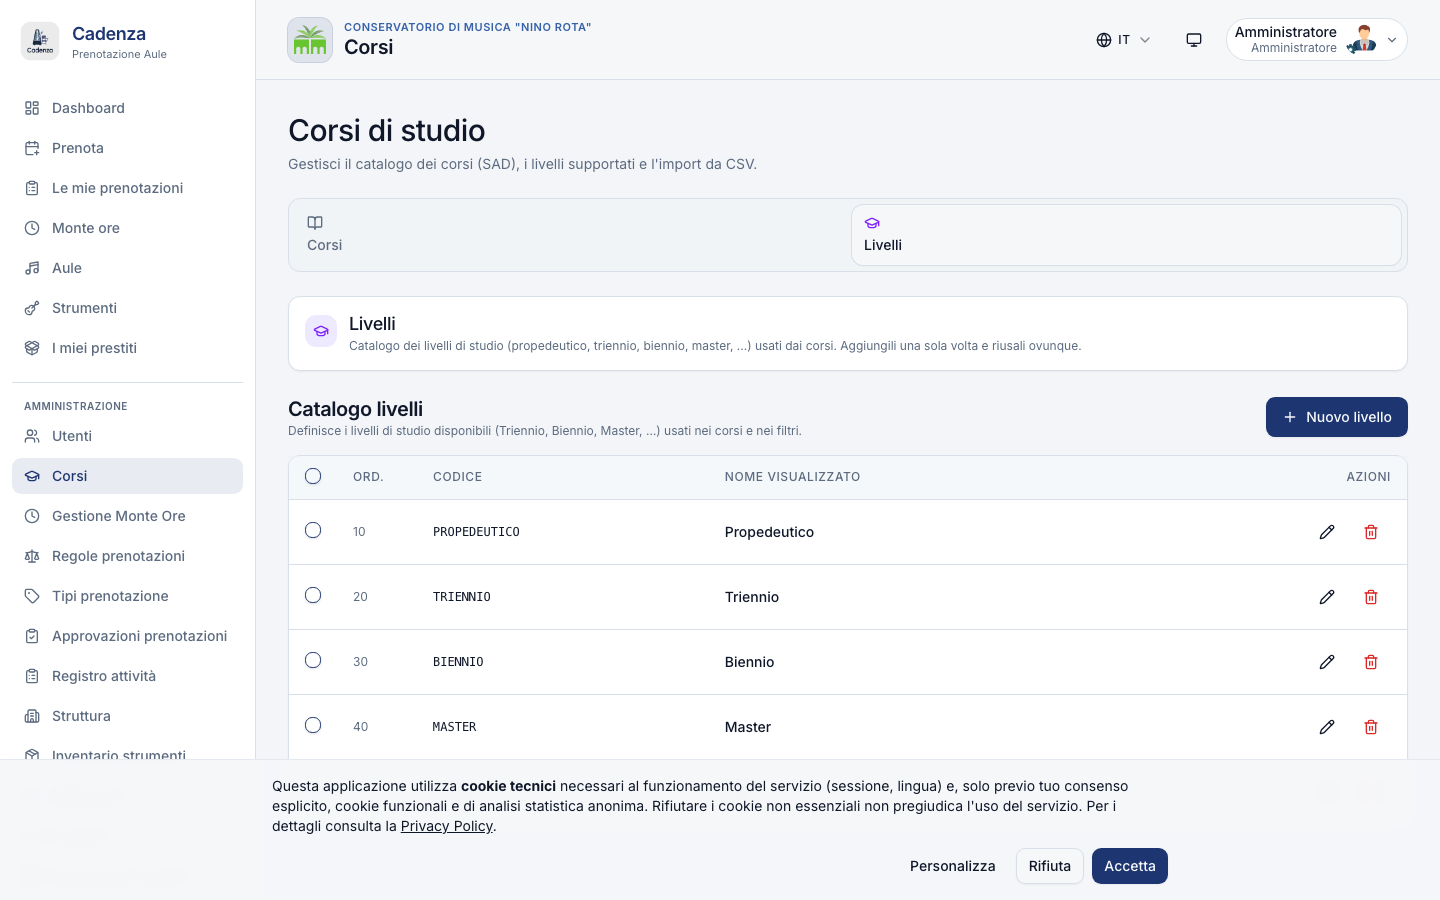
\includegraphics[width=0.95\linewidth]{screenshots/courses-livelli.png}\caption*{Tab Livelli — anagrafica dei livelli di studio (propedeutico, triennio, ecc.)}\end{figure}

Il catalogo dei livelli di studio (es. \texttt{propedeutico}, \texttt{triennio}, \texttt{biennio}, \texttt{master}). Una volta creato un livello lo riusi su tutti i corsi che lo supportano. Ogni livello ha codice, etichetta visualizzata, ordine in lista e stato attivo/disattivato.

\medskip\hrule\medskip

\section{5. Struttura: Istituti, Edifici, Aule, Dotazioni}


URL: \texttt{/admin/structure} (con scheda \texttt{?tab=sedi|dotazioni})

\subsection{5.1 Layout}


\begin{figure}[H]\centering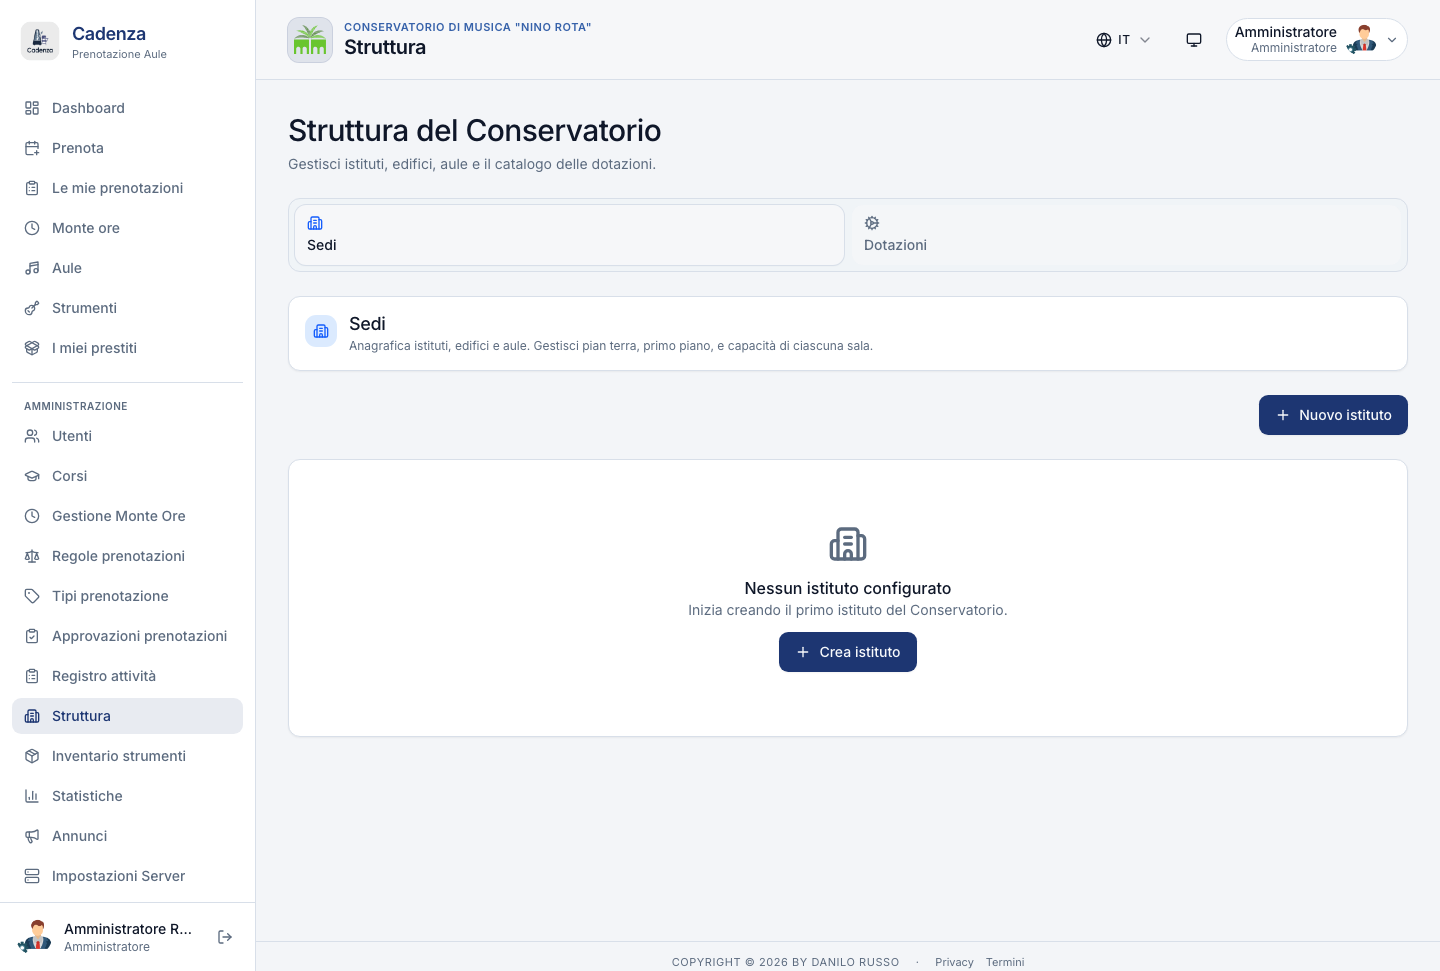
\includegraphics[width=0.95\linewidth]{screenshots/structure-sedi.png}\caption*{Tab Sedi — Istituto \textgreater{} Edificio \textgreater{} Aula con card espandibili e bottoni inline}\end{figure}

Macro-tab selector in alto: \textbf{Sedi} e \textbf{Dotazioni}.

La gerarchia è: \textbf{Istituto $\rightarrow$ Edificio $\rightarrow$ Aula $\rightarrow$ Equipment} (dotazione strumentale dell'aula). Ogni livello è una card espandibile/collassabile con anagrafica e i bottoni \textbf{+ Crea figlio}, \textbf{\textit{mod.} Modifica}, \textbf{\textit{canc.} Elimina}.

Le \textbf{dotazioni di una stanza} appaiono come "chip" cliccabili sotto la riga dell'aula (per modificare o cancellare al volo) con un bottone tratteggiato \textbf{+ Aggiungi}.

\subsection{5.2 Form Istituto}


Il form Istituto raccoglie l'anagrafica e i \textbf{dati legali} che servono alla pagina Privacy Policy / Termini.

\textbf{Anagrafica}: Nome, Codice, Città, Indirizzo, Descrizione, Logo (PNG/JPG/WEBP/SVG).

\textbf{Dati legali} (per la sezione "Titolare del trattamento" della privacy):

\begin{itemize}
  \item Denominazione legale ("Conservatorio di Musica Statale ...")
  \item P. IVA, Codice fiscale
  \item Email contatto, PEC
  \item Nome e email del DPO (Data Protection Officer)
  \item Foro competente (default: città dell'istituto)
  \item Sub-processor: lista dei fornitori esterni (es. SMTP provider, hosting), uno per riga, formato \texttt{Nome | Finalità | Localizzazione | URL DPA}
\end{itemize}

\subsection{5.3 Form Edificio}


Nome, Codice, Indirizzo, Piani (lista separata da virgole, es. \texttt{Piano Terra, 1º, 2º}).

\subsection{5.4 Form Aula}


\begin{table}[H]
\centering
\small
\begin{tabularx}{\linewidth}{|X|X|}
\hline
\rowcolor{tableheader} Campo & Descrizione \\
\hline
Nome & Es. \texttt{Aula 12} \\
\hline
Codice & Es. \texttt{A.101} (facoltativo) \\
\hline
Piano & Da scegliere fra i piani definiti per l'edificio \\
\hline
Capienza & Numero di persone \\
\hline
Tipologia & \texttt{studio}, \texttt{aula}, \texttt{concerto}, \texttt{ufficio} \\
\hline
Ruoli ammessi & Quali ruoli possono prenotarla \\
\hline
Corsi autorizzati & Se vuoi limitare l'accesso a specifici corsi (vuoto = tutti) \\
\hline
Foto aula & Immagine 16:9 (facoltativa) \\
\hline
Aula prenotabile & Disattiva temporaneamente l'aula da tutto il sistema \\
\hline
Richiedi check-in (QR) & Se attivo, l'utente deve scansionare un QR per "presentarsi" (anti-ghost). Se \textbf{disattivato}: niente auto-cancellazione dopo i 15 min di tolleranza, niente email "Prenotazione annullata: nessun check-in", niente badge "Senza check-in" su MyBookings, il bottone "Stampa QR aula" sparisce e la pagina \texttt{/check-in/room/:id} mostra il banner "Check-in non richiesto" \\
\hline
Richiede approvazione & Per le sale concerti / auditorium: ogni prenotazione passa per §7.1 \\
\hline
QR check-in (PDF) & Bottone per scaricare il foglio A4 da affiggere in aula \\
\hline
\end{tabularx}
\end{table}


\subsection{5.5 Form Dotazione (Equipment)}


Permette di descrivere lo strumentario di una specifica aula: nome, tipologia, quantità, marca/modello, in funzione (sì/no). Puoi pre-compilare nome e tipo scegliendo dal \textbf{catalogo dotazioni} (vedi §5.7).

\subsection{5.6 Bulk action floating bar}


Selezionando edifici o aule (checkbox), in basso compare una card fissa con i conteggi degli elementi selezionati e i bottoni \textbf{Deseleziona} ed \textbf{Elimina}. La cancellazione di un edificio rimuove a cascata anche le sue aule, le dotazioni e le prenotazioni; lo stesso vale per la cancellazione di un'aula. Cadenza ti riporta i conteggi finali nel toast (es. "5 aule eliminate, 12 prenotazioni rimosse").

\subsection{5.7 Tab "Dotazioni"}


\begin{figure}[H]\centering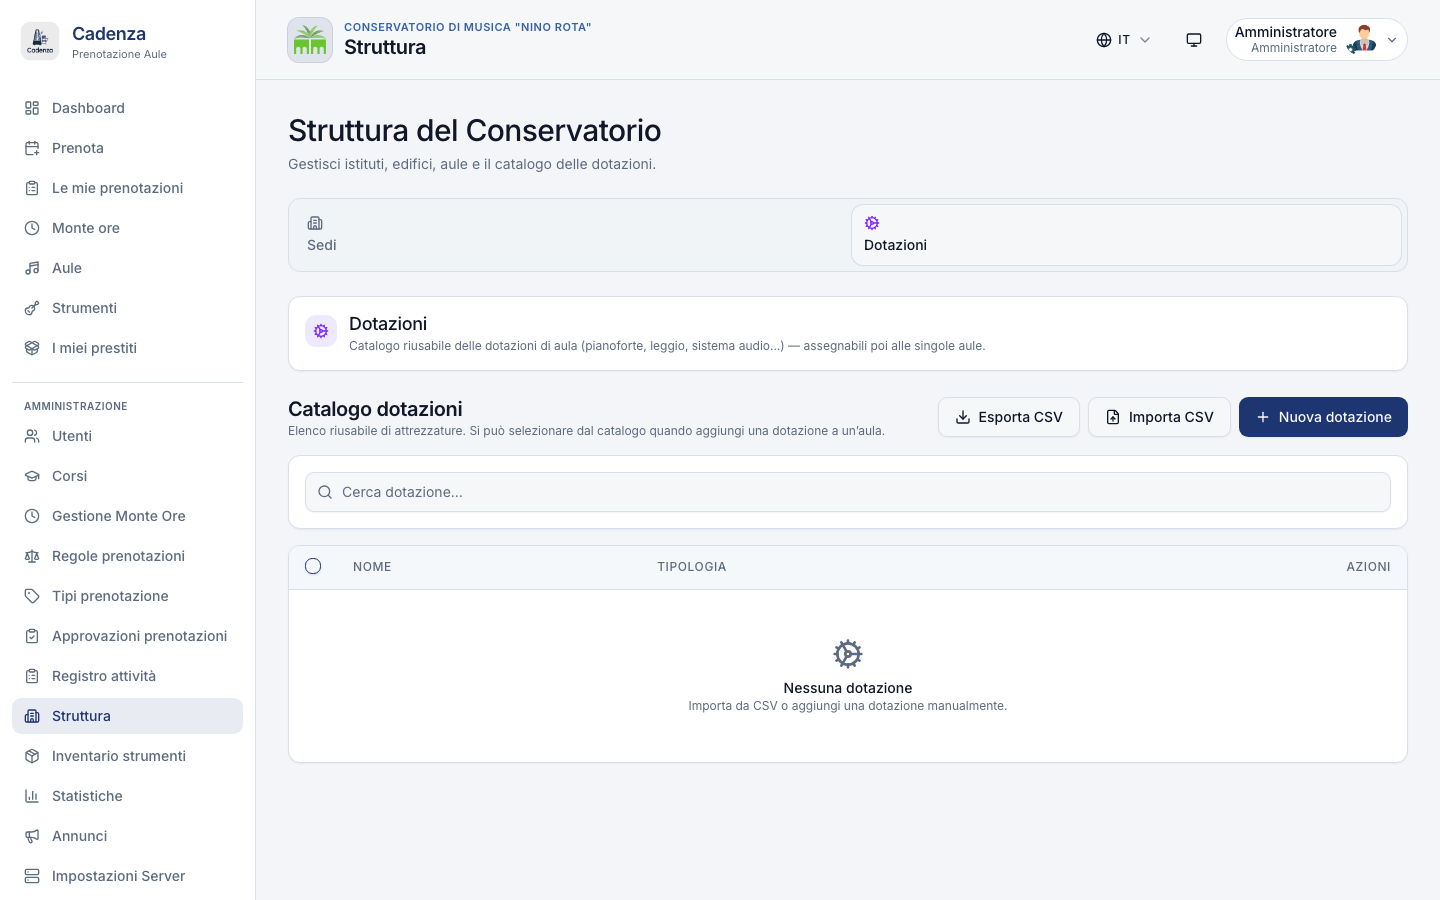
\includegraphics[width=0.95\linewidth]{screenshots/structure-dotazioni.png}\caption*{Tab Dotazioni — catalogo template riusabili da assegnare alle aule}\end{figure}

Il catalogo riusabile delle dotazioni (template). Una volta creato il template "Pianoforte verticale", lo riusi assegnandolo a tutte le aule che lo posseggono in due click. Cambiare il template aggiorna automaticamente tutte le aule che lo usano.

\subsection{5.8 Vista pubblica \texttt{/rooms}}


La pagina \texttt{/rooms} (visibile a tutti gli utenti loggati) mostra le aule \textbf{raggruppate per edificio}, con sezioni espandibili e un colore identificativo per ogni edificio. Riduce lo scroll su istituti con più sedi e rende immediato distinguere "Aula 12 --- Storico" da "Aula 12 --- Succursale". Lo stato espanso/collassato di ogni gruppo viene ricordato durante la sessione.

\medskip\hrule\medskip

\section{6. \textbf{[!]} Regole prenotazione}


URL: \texttt{/admin/rules}

Questa è la sezione che governa \textbf{chi può prenotare cosa, quando e per quanto tempo}. Le regole sono lo strato di policy che Cadenza applica a ogni nuova prenotazione: la prenotazione passa solo se \textbf{tutte} le regole applicabili la consentono.

\begin{figure}[H]\centering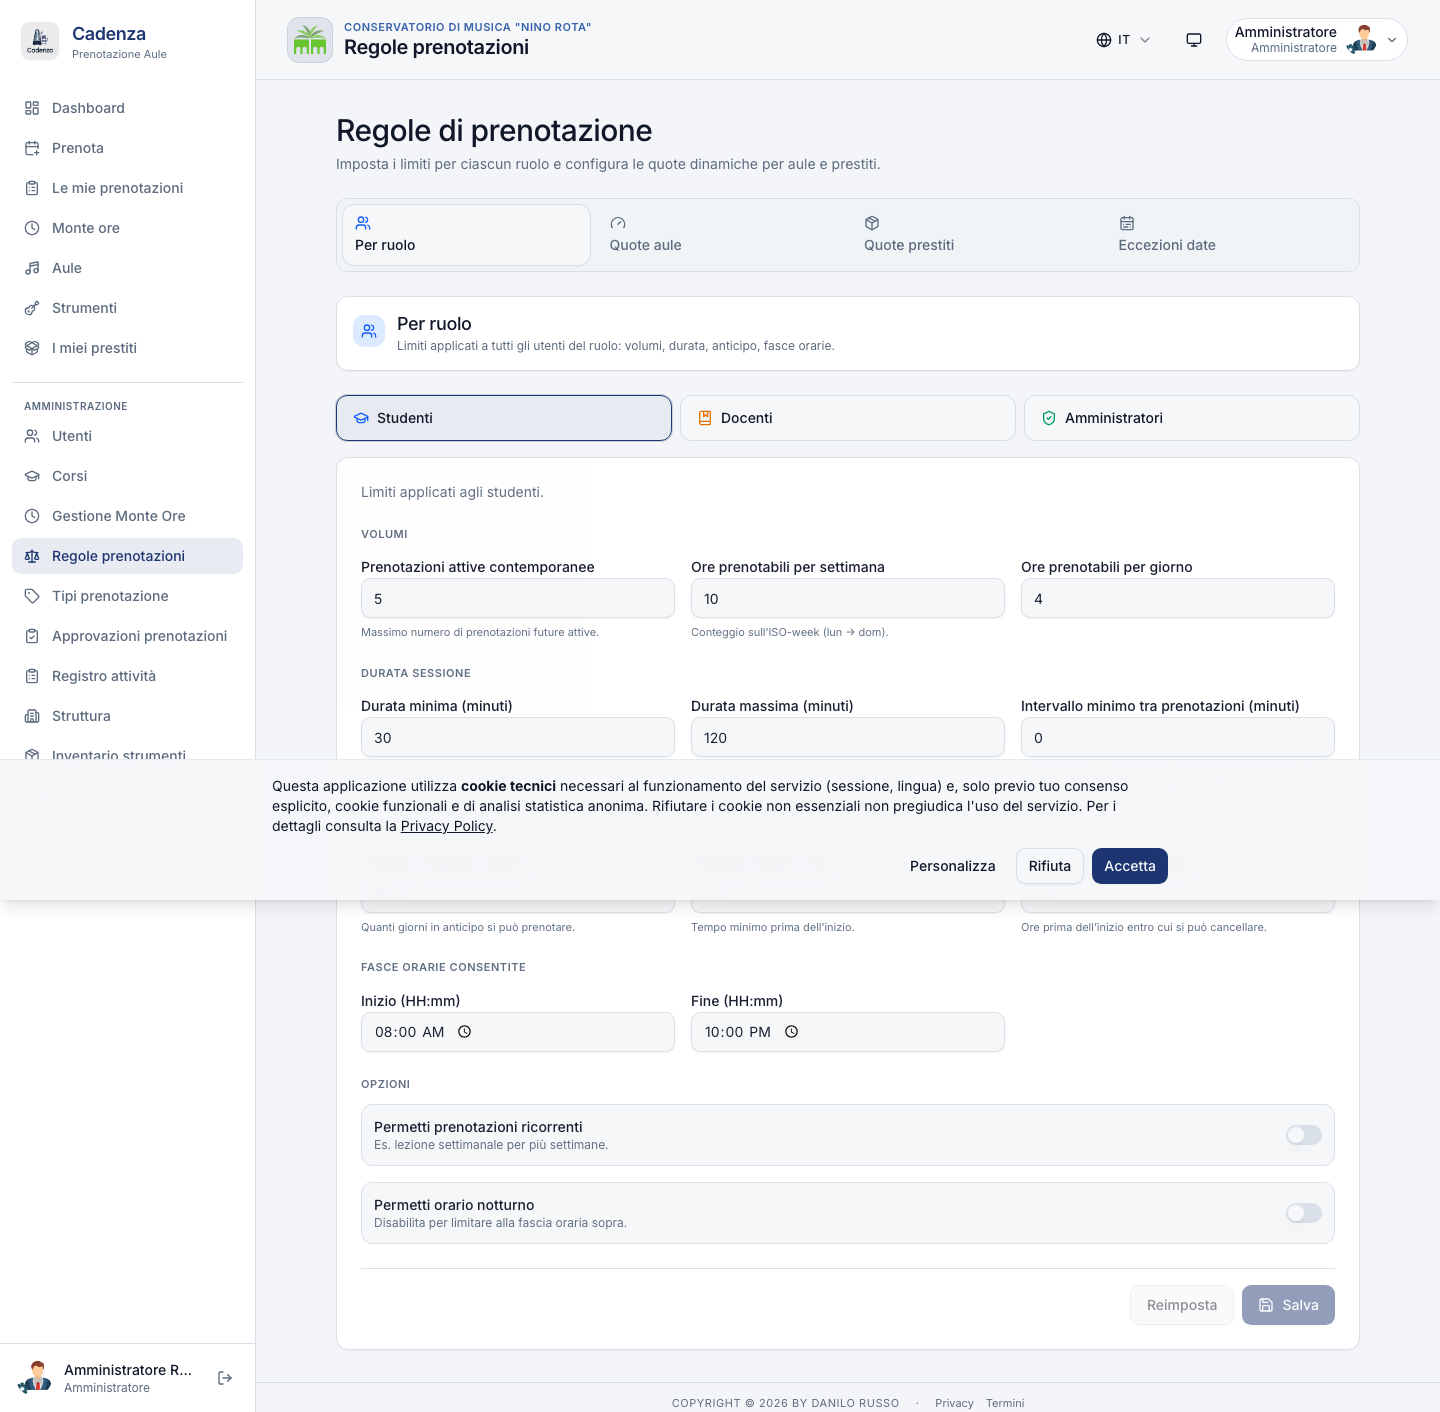
\includegraphics[width=0.95\linewidth]{screenshots/rules-overview.png}\caption*{Pagina Regole prenotazioni — vista d'insieme con 4 tab}\end{figure}

La pagina ha \textbf{quattro macro-tab} in alto:

\begin{lstlisting}
Regole prenotazioni
├─ Per ruolo            (limiti base per studenti / docenti / admin)
├─ Quote                (limiti per stanza / edificio / tipo aula)
├─ Quote prestiti       (analogo per inventario strumenti)
└─ Eccezioni            (override temporanei per ruolo, aula e finestra)
\end{lstlisting}

\subsection{6.0 Come Cadenza valuta una prenotazione (in sintesi)}


Quando un utente prova a prenotare, Cadenza verifica in ordine:

\begin{enumerate}
  \item L'utente è \textbf{attivo e approvato}.
  \item L'aula è \textbf{prenotabile} (non disattivata, non cestinata).
  \item Non c'è già \textbf{un'altra prenotazione} confermata sull'aula nella stessa fascia oraria.
  \item L'utente non ha \textbf{un'altra prenotazione confermata in un'altra aula} nella stessa fascia (un docente non può fisicamente essere in due posti).
  \item La regola \textbf{per ruolo} (max ore/settimana, durata massima, finestra oraria, cooldown, ecc.) è rispettata.
  \item Le \textbf{quote} specifiche (per tipo aula, stanza, edificio) sono rispettate.
  \item Nessuna \textbf{eccezione \texttt{block}} copre quella fascia oraria/aula/ruolo.
  \item Se l'aula richiede approvazione, la prenotazione viene salvata in stato \texttt{pending\_approval} (vedi §7.1).
\end{enumerate}

Se uno dei controlli fallisce, l'utente vede un messaggio leggibile nella propria interfaccia che spiega esattamente cosa non torna (es. "Hai superato le ore settimanali consentite").

\subsection{6.1 Tab "Per ruolo"}


\begin{figure}[H]\centering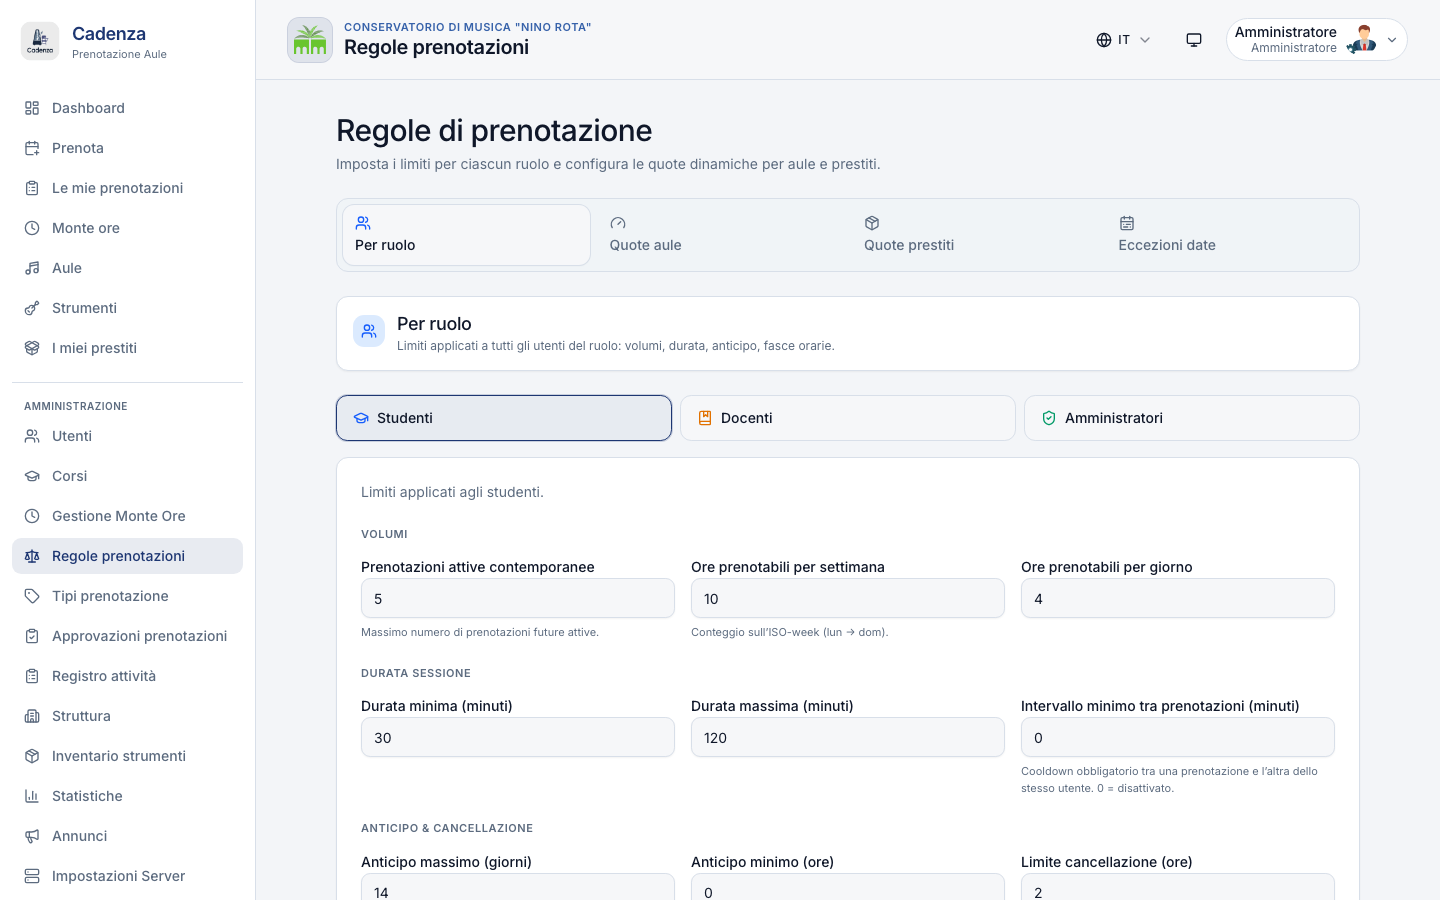
\includegraphics[width=0.95\linewidth]{screenshots/rules-per-ruolo.png}\caption*{Tab Per ruolo — limiti base per studenti, docenti e admin}\end{figure}

Tre toggle in alto per scegliere il ruolo (Studenti · Docenti · Admin). Sotto, un form con i parametri che valgono per quel ruolo:

\begin{table}[H]
\centering
\small
\begin{tabularx}{\linewidth}{|X|X|X|}
\hline
\rowcolor{tableheader} Campo & Default & Significato \\
\hline
\textbf{Max prenotazioni attive contemporanee} & 5 & Numero massimo di prenotazioni future contemporanee. \\
\hline
\textbf{Max ore / settimana} & 10 (studente), 20 (docente) & Tetto orario settimanale (lun--dom). \\
\hline
\textbf{Max ore / giorno} & 4 & Tetto giornaliero. \\
\hline
\textbf{Durata massima prenotazione} & 120 minuti & Una prenotazione di 3h va spezzata in più slot. \\
\hline
\textbf{Durata minima prenotazione} & 30 minuti & Slot minimo (allineato al granularità del calendario). \\
\hline
\textbf{Anticipo massimo (giorni)} & 14 & Quanto in anticipo si può prenotare. Studente=14, docente=30 tipici. \\
\hline
\textbf{Anticipo minimo (minuti)} & 0 & Per evitare prenotazioni "fra 5 minuti" su aule libere. Docente=0, studente=15 tipici. \\
\hline
\textbf{Cancellation cutoff (ore)} & 2 & Sotto questa soglia, cancellare conta come no-show (e va a impattare le statistiche). \\
\hline
\textbf{Richiede approvazione} & falso & Se vero, \textbf{tutte} le prenotazioni di quel ruolo passano per la coda di approvazione (utile per il primo periodo dei nuovi studenti). \\
\hline
\textbf{Allow same-day} & vero & Permettere prenotazioni in giornata. \\
\hline
\textbf{Orario apertura / chiusura} & 08:00 / 22:00 & Fuori finestra le prenotazioni vengono rifiutate. \\
\hline
\textbf{Cooldown tra prenotazioni} (minuti) & 0 & Minuti minimi tra la fine di una prenotazione e l'inizio della successiva dello stesso utente. Utile per evitare il "trucco" di concatenare due slot da 2h per fare di fatto un blocco da 4h. \\
\hline
\end{tabularx}
\end{table}


\subsubsection{Configurazione consigliata per la prima messa in opera}


\begin{lstlisting}
ruolo studente:
  max attivi=5, max settimanali=10h, max giornaliere=4h
  durata max=120 min, durata min=30 min
  anticipo max=14 gg, anticipo min=15 min, cutoff=2h
  no approvazione, no same-day=falso, 08:00–22:00

ruolo docente:
  max attivi=20, max settimanali=40h, max giornaliere=8h
  durata max=240 min, durata min=30 min
  anticipo max=60 gg, anticipo min=0, cutoff=2h
  no approvazione, allow same-day=vero, 07:00–23:00

ruolo admin:
  illimitato (lascia 0 o vuoto per "nessun limite")
  altro come docente
\end{lstlisting}

\begin{quote}
I campi a \texttt{0} significano "nessun limite". Non confonderli con "campo non valorizzato".
\end{quote}

\subsection{6.1bis Scenari guidati per la configurazione "Per ruolo"}


Per aiutarti a partire, ecco tre profili di Conservatorio reali e i parametri consigliati. Adattali poi alla tua realtà locale.

\subsubsection{Scenario A --- Conservatorio piccolo / medio ($\leq$ 200 studenti, 1 sede)}


\begin{table}[H]
\centering
\small
\begin{tabularx}{\linewidth}{|X|X|X|X|}
\hline
\rowcolor{tableheader} Parametro & Studente & Docente & Razionale \\
\hline
Max prenotazioni attive & 5 & 15 & Lo studente non deve "occupare" il calendario settimane in anticipo \\
\hline
Max ore / settimana & 12 & 30 & 2h al giorno × 6 giorni per lo studente è generoso \\
\hline
Max ore / giorno & 4 & 8 & Studente non studia per 8h, docente sì \\
\hline
Durata max prenotazione & 120 & 240 & Lo studente fa lezione + studio personale \\
\hline
Anticipo max (gg) & 14 & 60 & Il docente programma il semestre, lo studente vede 2 settimane \\
\hline
Anticipo min (min) & 15 & 0 & Lo studente deve "decidersi" 15 min prima \\
\hline
Cancel cutoff (h) & 2 & 2 & Sotto le 2h conta come no-show \\
\hline
Orario apertura/chiusura & 08-22 & 07-23 & Il docente inizia presto e chiude più tardi \\
\hline
Cooldown tra prenotazioni & 30 min & 0 & Anti-aggiramento del cap giornaliero per gli studenti \\
\hline
\end{tabularx}
\end{table}


\subsubsection{Scenario B --- Conservatorio grande (\textgreater{} 400 studenti, 2-3 sedi, sala concerti)}


Stessi parametri di A, con queste differenze:

\begin{itemize}
  \item \textbf{Max ore / settimana studente: 8} (più persone in coda $\rightarrow$ ognuno ne usa di meno)
  \item \textbf{Max ore / giorno studente: 3}
  \item \textbf{Anticipo max studente: 7 gg} (rotazione più rapida)
  \item Aggiungi una \textbf{quota dedicata} sulle aule "premium" (vedi §6.2 esempio Q3)
  \item Considera il \textbf{cooldown 60 min} per gli studenti se vedi che concatenano sistematicamente
\end{itemize}

\subsubsection{Scenario C --- Sessione esami / saggi (modalità intensiva, 2-3 settimane all'anno)}


Non cambiare le regole base. Crea invece \textbf{eccezioni temporanee} (vedi §6.3) per:

\begin{itemize}
  \item Sospendere quota weekend (\texttt{time\_window} con \texttt{daysOfWeek=sab+dom}, \texttt{Ore max=999})
  \item Aprire l'orario serale fino alle 24 per i docenti (eccezione su ruolo docente)
  \item Limitare l'aula concerti a "solo prenotazioni dell'esame" (eccezione \texttt{block} con scope aula)
\end{itemize}

Le eccezioni scadono in automatico alla data finale: niente da ricordare di ripristinare a posteriori.

\subsection{6.2 Tab "Quote"}


\begin{figure}[H]\centering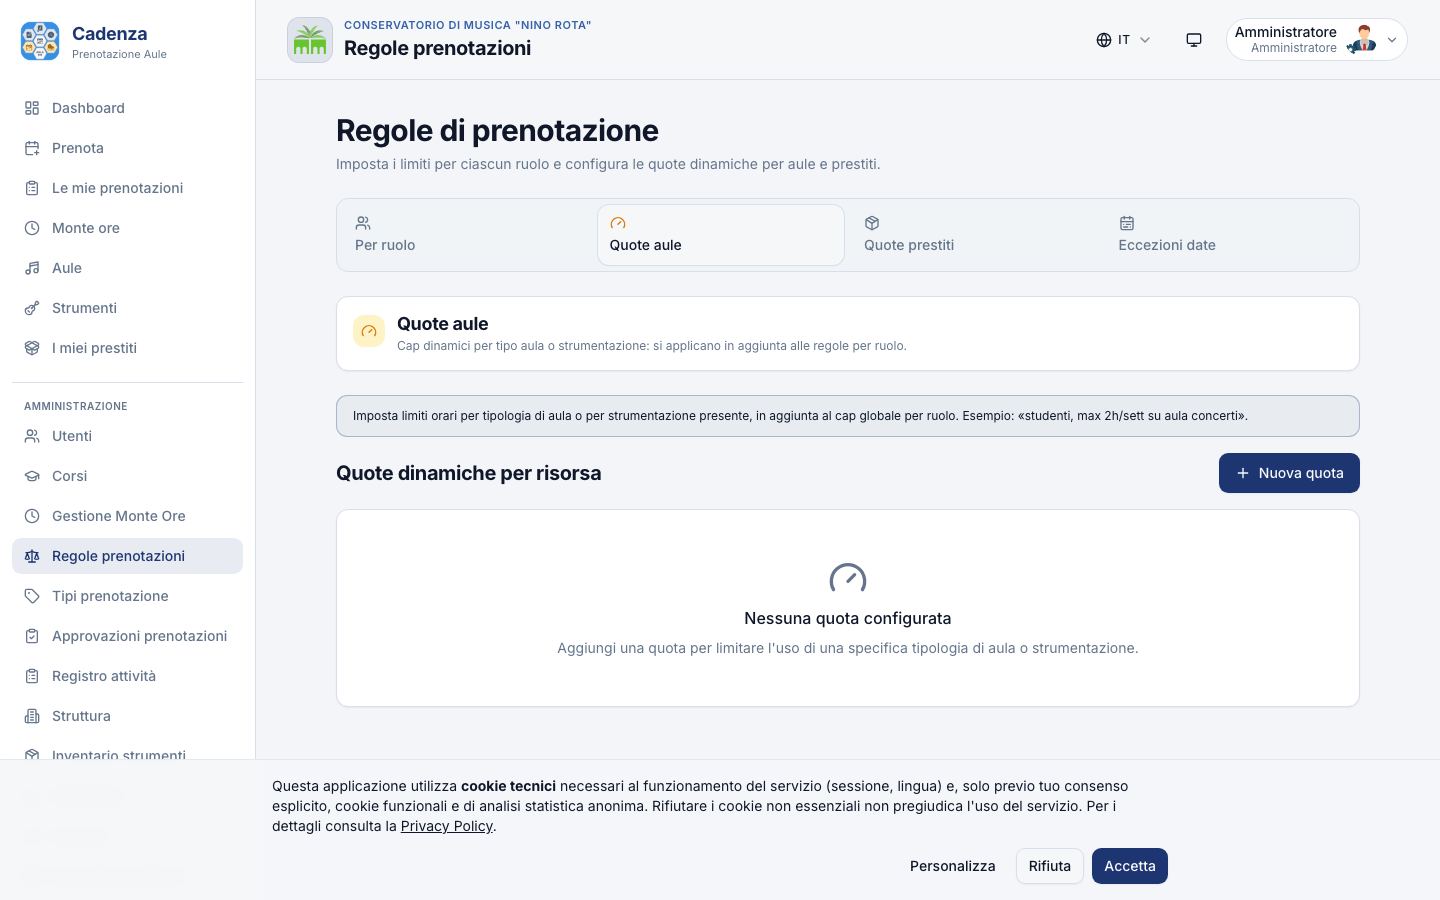
\includegraphics[width=0.95\linewidth]{screenshots/rules-quote.png}\caption*{Tab Quote — limiti granulari per stanza, edificio, tipo aula}\end{figure}

Una \textbf{quota} è un sotto-limite più stringente per uno specifico target. Cadenza applica \textbf{prima} la regola per ruolo e \textbf{poi} tutte le quote che corrispondono al target della prenotazione, prendendo il limite più basso.

\begin{quote}
\textbf{In una frase}: "\_la regola di ruolo dice quanto vale per tutto il sistema; la quota dice quanto vale per una specifica risorsa\_". Se per uno studente il ruolo dice 12 h/sett ma esiste una quota "Aula 12: max 2h/sett per studente", quello studente farà al massimo 2h in Aula 12 + altre 10h sparse altrove.
\end{quote}

\subsubsection{Tipi di scope}


\begin{table}[H]
\centering
\small
\begin{tabularx}{\linewidth}{|X|X|X|}
\hline
\rowcolor{tableheader} Scope & Esempio & Uso tipico \\
\hline
\texttt{roomType} & studio · aula · concerto & "Studenti possono prenotare la sala concerti max 4h/settimana" \\
\hline
\texttt{equipmentType} & pianoforte\_coda · contrabbasso & "Solo pianisti possono prenotare aule con pianoforte a coda" \\
\hline
\texttt{room} & aula 101 & Limite specifico su una stanza (es. la più richiesta) \\
\hline
\texttt{building} & edificio\_centrale & Limite per edificio (utile se uno è in ristrutturazione) \\
\hline
\texttt{global} & * & Limite globale (oltre quello di ruolo) \\
\hline
\end{tabularx}
\end{table}


\subsubsection{Tetti che puoi mettere su una quota}


Ogni quota può combinare uno o più di questi tetti --- Cadenza applica il \textbf{più stringente} che trova:

\begin{table}[H]
\centering
\small
\begin{tabularx}{\linewidth}{|X|X|}
\hline
\rowcolor{tableheader} Tetto & Significato \\
\hline
Max ore / giorno & Tetto giornaliero su quel target \\
\hline
Max ore / settimana & Tetto settimanale (lun--dom) \\
\hline
Max ore / mese & Tetto del mese solare \\
\hline
Max prenotazioni & Numero massimo di prenotazioni nel periodo \\
\hline
Giorni della settimana & Lista giorni cui si applica (vuoto = tutti) \\
\hline
Fascia oraria & Inizio -- Fine entro cui la quota agisce \\
\hline
\end{tabularx}
\end{table}


\begin{quote}
Almeno \textbf{un tetto} \textgreater{} 0 deve essere presente: una quota "0 ore in tutto" significa "blocca completamente quel target per quel ruolo" e ha un nome dedicato (eccezione \texttt{block}, vedi §6.3).
\end{quote}

\subsubsection{Esempi pratici di quote}


\begin{table}[H]
\centering
\small
\begin{tabularx}{\linewidth}{|X|X|X|X|X|X|X|X|}
\hline
\rowcolor{tableheader} \# & Ruolo & Scope & Scope value & Tetto & Giorni & Orario & Note \\
\hline
Q1 & studente & \texttt{roomType} & concerto & 0 & tutti & --- & Studenti non possono prenotare sale concerti \\
\hline
Q2 & docente & \texttt{roomType} & concerto & 4 h/mese & tutti & --- & Docenti: sala concerti solo per prove serie \\
\hline
Q3 & studente & \texttt{room} & "Aula 12 --- Pianoforte coda" & 2 h/sett & tutti & --- & Aula contesa: massimo 2h/settimana per studente \\
\hline
Q4 & studente & \texttt{global} & * & 6 h totali & sab-dom & --- & Limite weekend: 6h totali sab + dom \\
\hline
Q5 & studente & \texttt{building} & "Sede succursale" & 0 & tutti & --- & Edificio in ristrutturazione \\
\hline
Q6 & studente & \texttt{equipmentType} & pianoforte\_coda & 4 h/sett & tutti & --- & Solo se studente di pianoforte può prenotare il "coda" \\
\hline
Q7 & docente & \texttt{roomType} & concerto & 8 h/sett & tutti & 18:00--22:00 & Concerto disponibile solo la sera per i docenti \\
\hline
Q8 & studente & \texttt{room} & "Sala 3 --- Sala prove" & 3 h/giorno · 9 h/sett & tutti & 09:00--22:00 & Limite giornaliero + settimanale combinati \\
\hline
\end{tabularx}
\end{table}


\subsubsection{Sequenza di applicazione (cosa succede passo-passo)}


Quando uno studente prova a prenotare 2h in Aula 12 (pianoforte coda) il martedì dalle 14 alle 16, Cadenza fa così:

\begin{enumerate}
  \item Verifica la regola di ruolo (es. studente: max 12 h/sett · max 4 h/giorno) $\rightarrow$ OK ammesso ne ha già fatte 8 nella settimana e 0 nella giornata.
  \item Cerca le quote che riguardano questa prenotazione: - Q3 \texttt{room} "Aula 12" --- max 2 h/sett $\rightarrow$ contiamo le ore già prenotate in Aula 12 questa settimana - Q6 \texttt{equipmentType} pianoforte\_coda --- max 4 h/sett $\rightarrow$ contiamo le ore in qualunque aula con questa dotazione
  \item \textbf{Limite più stretto vince}. Se Q3 dice ne ha già 1h e Q6 dice 2h: - Q3 ammette ancora 1h - Q6 ammette ancora 2h - \textbf{Cadenza accetta solo 1h} (il minimo dei due) $\rightarrow$ l'utente vede "Hai raggiunto il limite per Aula 12".
  \item Se nulla blocca, la prenotazione viene salvata (oppure va in approvazione se l'aula lo richiede).
\end{enumerate}

\begin{quote}
\textbf{Quote vs eccezioni}: la quota è \textbf{strutturale e permanente} ("Aula 12 vale così tutto l'anno"). L'eccezione è \textbf{temporanea} ("dal 1 al 30 giugno cambiamo le regole"). Vedi §6.3 per le eccezioni.
\end{quote}

\subsection{6.2bis Tab "Quote prestiti"}


\begin{figure}[H]\centering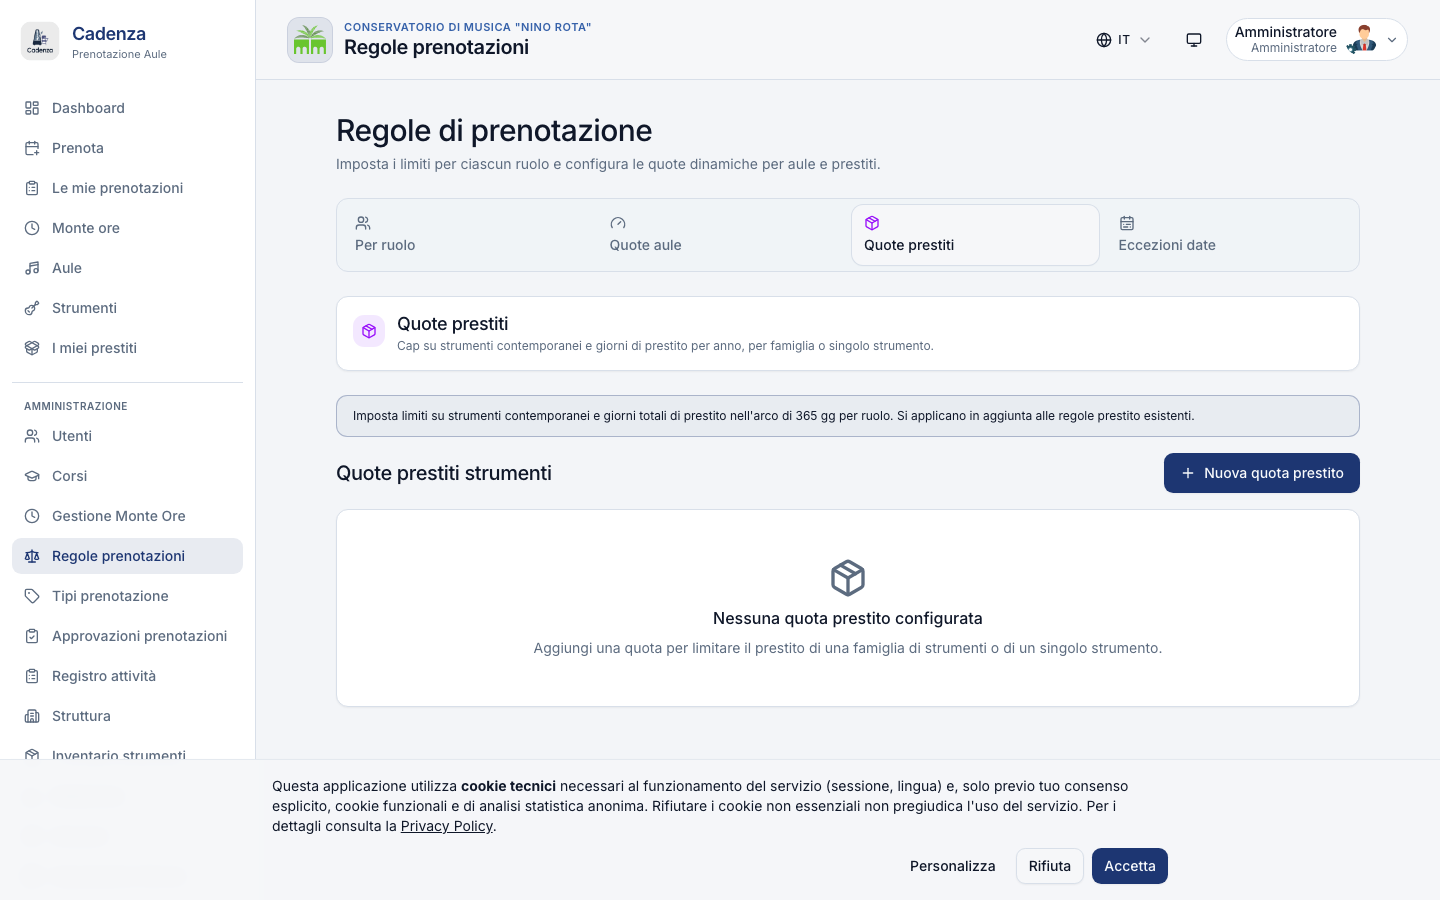
\includegraphics[width=0.95\linewidth]{screenshots/rules-quote-prestiti.png}\caption*{Tab Quote prestiti — limiti per famiglia, strumento e globali sull'inventario}\end{figure}

Stesso schema delle quote aule, ma applicato all'\textbf{inventario strumenti}:

\begin{table}[H]
\centering
\small
\begin{tabularx}{\linewidth}{|X|X|}
\hline
\rowcolor{tableheader} Campo & Significato \\
\hline
Ruolo & Admin · Docente · Studente \\
\hline
Scope & \texttt{family} (archi, fiati, ecc.) · \texttt{instrument} · \texttt{global} \\
\hline
Max simultanei & Quanti prestiti aperti contemporaneamente \\
\hline
Max giorni anno & Quanti giorni cumulati in un anno solare \\
\hline
Attivo & Disabilita la quota senza eliminarla \\
\hline
\end{tabularx}
\end{table}


\subsection{6.3 Tab "Eccezioni"}


\begin{figure}[H]\centering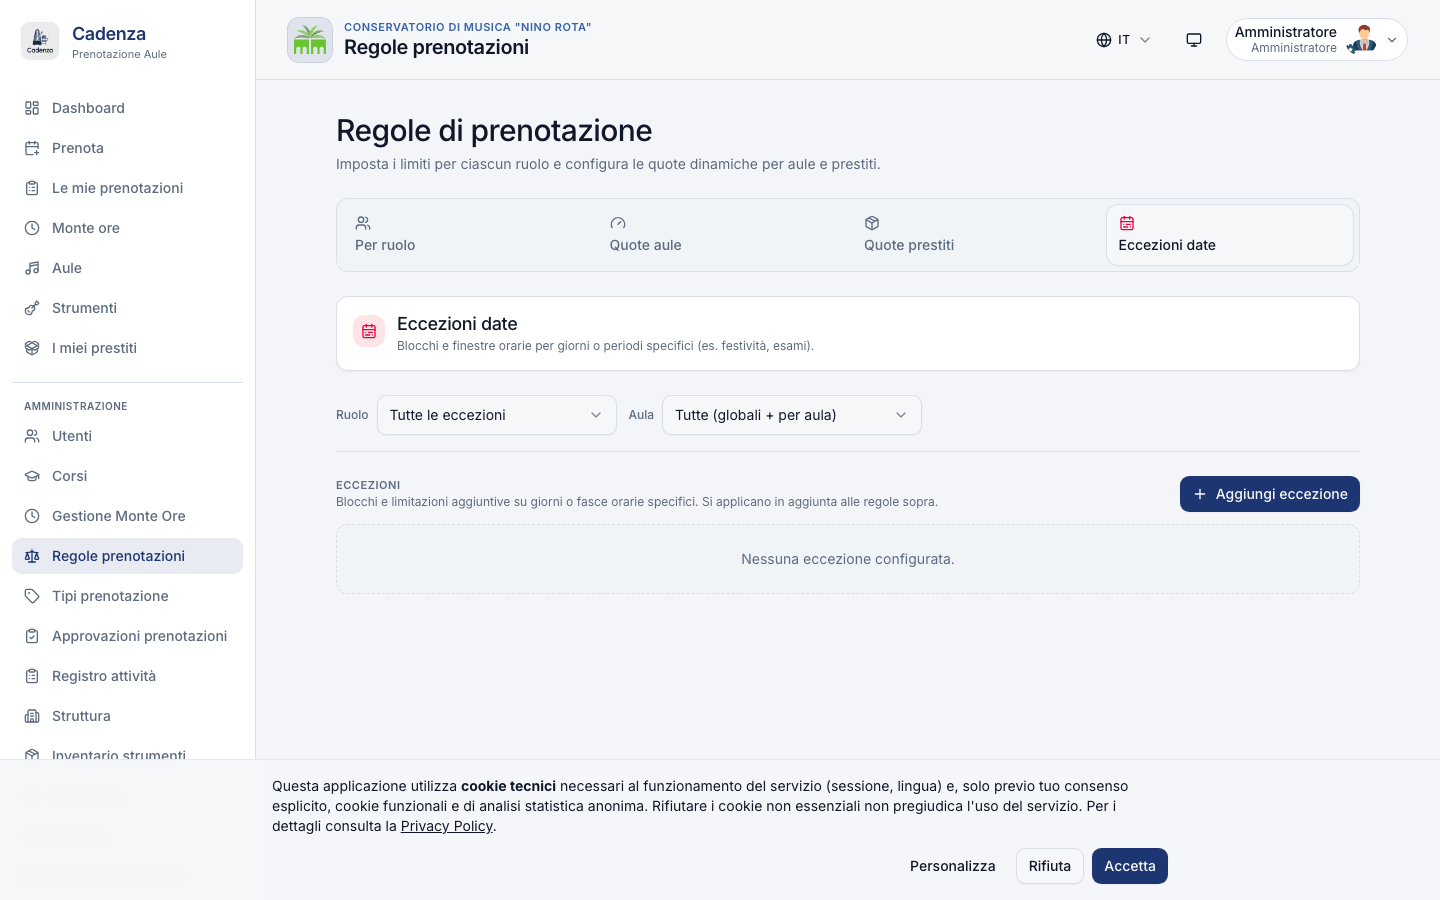
\includegraphics[width=0.95\linewidth]{screenshots/rules-eccezioni.png}\caption*{Tab Eccezioni — override temporanei per utenti o aule specifiche}\end{figure}

Le eccezioni sono \textbf{regole temporanee} che entrano in gioco al posto (o in aggiunta) di quelle normali. La differenza con le quote di §6.2 è la \textbf{scadenza}: una quota vale finché non la cancelli; un'eccezione ha una data di inizio e una di fine.

Le eccezioni \textbf{sospendono o sostituiscono} una regola/quota per:

\begin{itemize}
  \item una \textbf{finestra temporale} specifica (es. "durante la sessione esami sospendi la quota weekend")
  \item uno \textbf{specifico ruolo} (es. "tutti gli studenti dal 1 al 15 giugno")
  \item una \textbf{specifica aula} \textbf{[!]} NUOVO (es. "Aula 5: max 2h/giorno per gli studenti dal 1 al 30 giugno")
  \item una combinazione delle precedenti (ruolo + aula + finestra)
\end{itemize}

L'eccezione ha priorità sulla regola/quota originaria. Ogni modifica viene tracciata nel registro attività.

\subsubsection{Due tipi di eccezione}


Cadenza supporta due tipi di eccezione, da scegliere al momento della creazione:

\begin{table}[H]
\centering
\small
\begin{tabularx}{\linewidth}{|X|X|X|}
\hline
\rowcolor{tableheader} Tipo & Cosa fa & Caso d'uso tipico \\
\hline
\texttt{block} & \textbf{Chiusura totale} del target nella finestra. Nessuna prenotazione passa. & Aula in ristrutturazione, sciopero, festa patronale, evento istituzionale che occupa l'intera struttura \\
\hline
\texttt{time\_window} & \textbf{Cambia il limite di ore} nella finestra. La prenotazione passa solo se sotto il nuovo tetto. Può \textbf{rilassare} (più ore del solito) o \textbf{stringere} (meno ore) rispetto alla regola normale. & Sessione esami: "lo studente può fare 999h/sett (di fatto illimitato)" oppure "Aula 5 a numero chiuso: max 2h/giorno per studente" \\
\hline
\end{tabularx}
\end{table}


\subsubsection{Lista eccezioni --- toolbar e filtri}


In alto sopra la tabella:

\begin{itemize}
  \item \textbf{Filtro Ruolo}: tutti i ruoli · studenti · docenti · admin.
  \item \textbf{Filtro Aula}: tutte le aule · oppure scegli una specifica aula. Le aule sono ordinate \texttt{Sede · Aula} (es. "Conservatorio Storico · Aula 12") per non confondersi quando ci sono numeri ripetuti tra edifici diversi.
\end{itemize}

\begin{quote}
Le aule la cui Sede è stata cestinata da \texttt{/admin/structure} non compaiono nei due Select.
\end{quote}

Ogni riga della lista mostra: nome dell'eccezione + tipo (\texttt{block} viola scuro · \texttt{time\_window} ambra), il badge ruolo, il badge viola \textbf{"Aula X"} se è scoped, la finestra date e l'icona attiva/non attiva.

\subsubsection{Form Eccezione}


\begin{figure}[H]\centering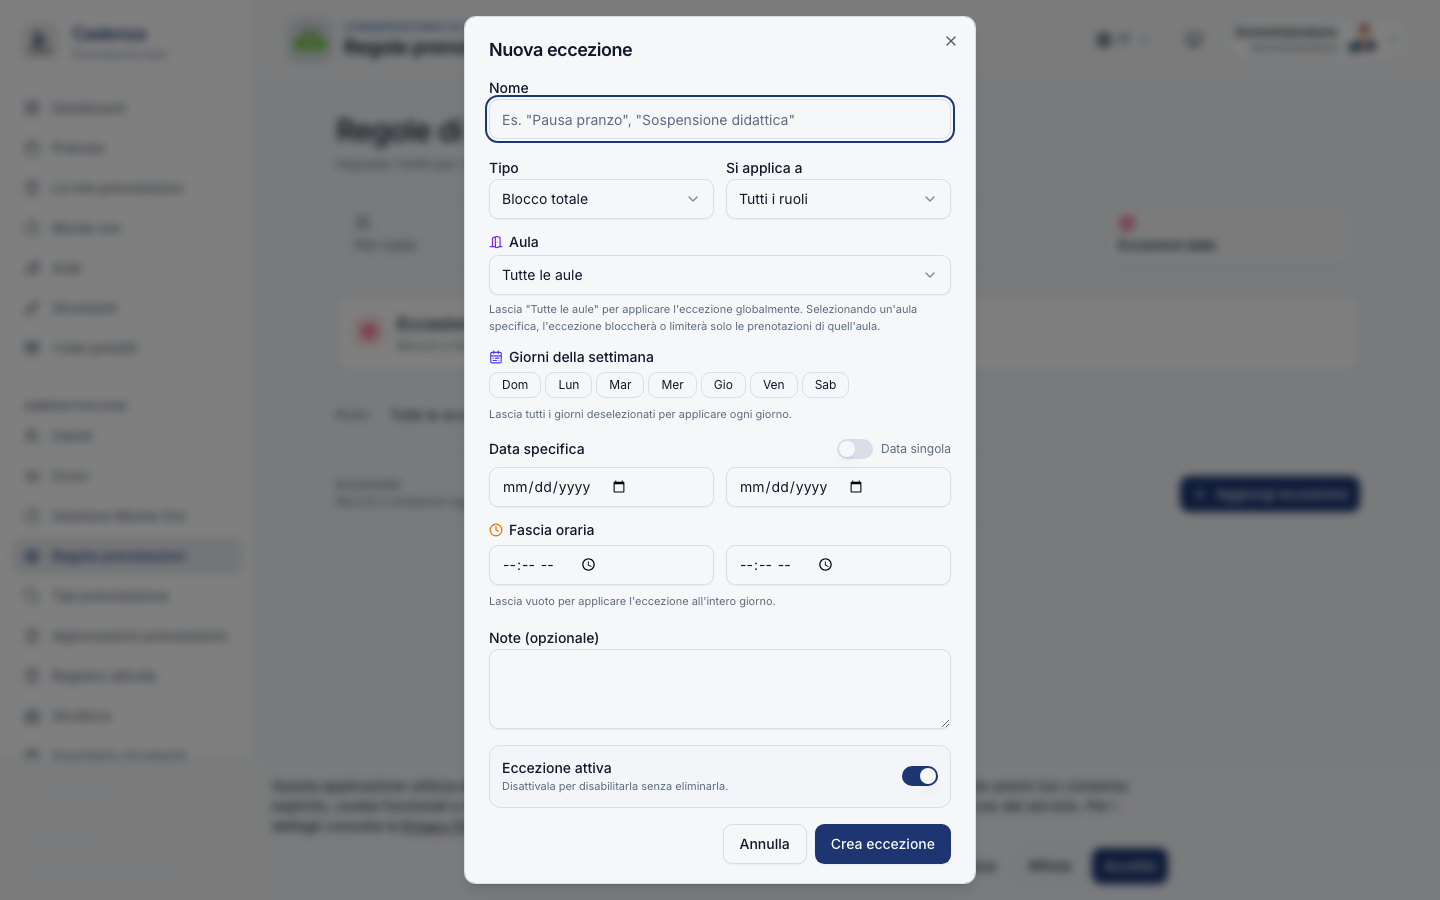
\includegraphics[width=0.95\linewidth]{screenshots/rules-eccezione-dialog.png}\caption*{Dialog Nuova Eccezione — campi del form, incluso il Select Aula}\end{figure}

\begin{table}[H]
\centering
\small
\begin{tabularx}{\linewidth}{|X|X|}
\hline
\rowcolor{tableheader} Campo & Descrizione \\
\hline
Nome & Etichetta libera (es. "Saggi sessione estiva") \\
\hline
Tipo & \texttt{block} (chiusura totale) oppure \texttt{time\_window} (limite ore in una finestra) \\
\hline
Si applica a & Tutti · solo studenti · solo docenti · solo admin \\
\hline
\textbf{Aula} \textbf{[!]} NUOVO & Tutte le aule (default) oppure una specifica aula \\
\hline
Ore max nella finestra & Solo se \texttt{time\_window} (es. 2 ore) \\
\hline
Giorni della settimana & 7 bottoni Lun--Dom; vuoto = ogni giorno \\
\hline
Data singola / range & Toggle: data unica oppure dal--al \\
\hline
Fascia oraria & Inizio -- Fine (facoltativa) \\
\hline
Note & Testo libero \\
\hline
Attivo & Spegni per disabilitarla senza eliminarla \\
\hline
\end{tabularx}
\end{table}


\begin{quote}
\textbf{Pre-popolamento aula}: se apri il dialog mentre il filtro lista "Aula" è valorizzato, il Select del form parte già su quella aula.
\end{quote}

\begin{quote}
\textbf{Semantica scope aula}:  - \texttt{block} con aula scoped $\rightarrow$ blocca solo prenotazioni su quell'aula (es. ristrutturazione di una singola aula); le altre aule restano libere. - \texttt{time\_window} con aula scoped $\rightarrow$ "max X ore \textbf{in quell'aula}". Esempio: "Aula 12: max 2h/giorno per studente, dal 1 al 30 giugno" non impedisce di fare altre 2h nell'Aula 5 lo stesso giorno. - Aula = "Tutte" $\rightarrow$ la regola vale \textbf{per tutte le aule} (eccezione globale).
\end{quote}

\begin{quote}
\textbf{Nudge visivo}: se la data finale è nel passato, un banner azzurro avvisa che l'eccezione ignorerà comunque le nuove prenotazioni.
\end{quote}

\subsubsection{Scenari guidati per le eccezioni}


I 6 casi più frequenti, con i parametri esatti da inserire nel form:

\paragraph{Scenario 1 --- Aula in ristrutturazione (1 settimana)}


\begin{quote}
\textit{"L'Aula 7 viene tinteggiata dal 12 al 18 maggio. Nessuno deve prenotarla."}
\end{quote}

\begin{table}[H]
\centering
\small
\begin{tabularx}{\linewidth}{|X|X|}
\hline
\rowcolor{tableheader} Campo & Valore \\
\hline
Nome & "Aula 7 --- tinteggiatura" \\
\hline
Tipo & \texttt{block} \\
\hline
Si applica a & Tutti \\
\hline
Aula & "Sede Storica · Aula 7" \\
\hline
Dal · Al & 2026-05-12 · 2026-05-18 \\
\hline
Note & "Riapertura prevista lunedì 19" \\
\hline
\end{tabularx}
\end{table}


\begin{quote}
Al salvataggio Cadenza ti chiede se ci sono già prenotazioni in quel range. Vedi più sotto \textbf{"Sovrapposizioni storiche"}.
\end{quote}

\paragraph{Scenario 2 --- Sessione esami: weekend illimitato per docenti (2 settimane)}


\begin{quote}
\textit{"Dal 10 al 25 giugno i docenti possono prenotare anche sabato/domenica senza il tetto weekend di 6h."}
\end{quote}

\begin{table}[H]
\centering
\small
\begin{tabularx}{\linewidth}{|X|X|}
\hline
\rowcolor{tableheader} Campo & Valore \\
\hline
Nome & "Esami giugno --- weekend libero docenti" \\
\hline
Tipo & \texttt{time\_window} \\
\hline
Si applica a & Solo docenti \\
\hline
Aula & Tutte le aule \\
\hline
Ore max nella finestra & 999 (di fatto illimitato) \\
\hline
Giorni & sab + dom \\
\hline
Dal · Al & 2026-06-10 · 2026-06-25 \\
\hline
\end{tabularx}
\end{table}


\paragraph{Scenario 3 --- Sala concerti riservata per saggio finale (1 giorno)}


\begin{quote}
\textit{"Il 15 giugno la sala concerti è prenotabile SOLO da chi ha l'esame, dalle 18 alle 23."}
\end{quote}

Combo di due eccezioni:

\begin{enumerate}
  \item \texttt{block} su sala concerti per tutti dalle 00 alle 18 + dalle 23 alle 24 $\rightarrow$ la sala è chiusa fuori orario.
  \item Prenoti tu (admin) la sala concerti per il candidato --- la prenotazione passa perché un admin può sempre forzare se serve.
\end{enumerate}

In alternativa, più rapida: una singola eccezione \texttt{block} su tutte le aule \textbf{eccetto} chi ha già la prenotazione manuale fatta dall'admin (Cadenza non blocca le prenotazioni create prima dell'eccezione).

\paragraph{Scenario 4 --- Aula contesa: numero chiuso temporaneo (1 mese)}


\begin{quote}
\textit{"L'Aula 12 (con il pianoforte coda) è troppo richiesta a maggio. Limitiamola a max 2h/giorno per studente, dal 1 al 31 maggio."}
\end{quote}

\begin{table}[H]
\centering
\small
\begin{tabularx}{\linewidth}{|X|X|}
\hline
\rowcolor{tableheader} Campo & Valore \\
\hline
Nome & "Aula 12 --- numero chiuso maggio" \\
\hline
Tipo & \texttt{time\_window} \\
\hline
Si applica a & Solo studenti \\
\hline
Aula & "Sede Storica · Aula 12" \\
\hline
Ore max nella finestra & 2 (= max 2h/giorno) \\
\hline
Giorni & tutti \\
\hline
Dal · Al & 2026-05-01 · 2026-05-31 \\
\hline
\end{tabularx}
\end{table}


\begin{quote}
Importante: la finestra "ore max" qui è interpretata come \textbf{massimo per giorno} (la finestra giornaliera). Per cambiarla in settimanale, usa una quota in §6.2 invece di un'eccezione.
\end{quote}

\paragraph{Scenario 5 --- Vacanze di Natale: chiusura totale (2 settimane)}


\begin{quote}
\textit{"Dal 24 dicembre al 6 gennaio nessuno deve poter prenotare niente."}
\end{quote}

\begin{table}[H]
\centering
\small
\begin{tabularx}{\linewidth}{|X|X|}
\hline
\rowcolor{tableheader} Campo & Valore \\
\hline
Nome & "Chiusura natalizia" \\
\hline
Tipo & \texttt{block} \\
\hline
Si applica a & Tutti \\
\hline
Aula & Tutte le aule \\
\hline
Dal · Al & 2026-12-24 · 2027-01-06 \\
\hline
\end{tabularx}
\end{table}


\begin{quote}
In alternativa puoi usare il modulo Monte Ore $\rightarrow$ tab Sospensioni (§8.4): più ricco, perché ti gestisce anche gli slot Monte Ore esistenti.
\end{quote}

\paragraph{Scenario 6 --- Sciopero / festa patronale (1 giorno)}


\begin{quote}
\textit{"Il 16 ottobre è la festa di Santa Cecilia, patrona dei musicisti. Conservatorio chiuso."}
\end{quote}

\begin{table}[H]
\centering
\small
\begin{tabularx}{\linewidth}{|X|X|}
\hline
\rowcolor{tableheader} Campo & Valore \\
\hline
Nome & "Santa Cecilia 2026" \\
\hline
Tipo & \texttt{block} \\
\hline
Si applica a & Tutti \\
\hline
Aula & Tutte le aule \\
\hline
Dal · Al & 2026-10-16 (singola) \\
\hline
\end{tabularx}
\end{table}


\subsubsection{Combinazione di più eccezioni}


Le eccezioni sono \textbf{additive}: tutte quelle che corrispondono al target della prenotazione vengono valutate. Se due eccezioni si toccano:

\begin{itemize}
  \item Due \texttt{block} $\rightarrow$ l'utente vede comunque "aula chiusa".
  \item Un \texttt{block} + un \texttt{time\_window} $\rightarrow$ vince il \texttt{block} (il blocco totale è più stringente).
  \item Due \texttt{time\_window} $\rightarrow$ vince il limite più basso.
\end{itemize}

Esempio: hai un'eccezione "Aula 12 max 2h/giorno per maggio" (Scenario 4) e ne crei una seconda "Esami giugno --- weekend libero" (Scenario 2). Per uno studente che prova a prenotare l'Aula 12 il sabato 1 giugno, vale solo la prima (la seconda è per docenti).

\subsubsection{Sovrapposizioni storiche al setup di chiusure}


Quando crei un'eccezione di tipo \textbf{\texttt{block}} (chiusura aula/edificio per ristrutturazione, sciopero, festa patronale), Cadenza ti chiede subito \textbf{"ci sono prenotazioni già confermate che cadono in questo blocco?"}:

\begin{enumerate}
  \item Salvi l'eccezione.
  \item Si apre un dialog di follow-up con l'elenco delle prenotazioni in conflitto. Quelle collegate al piano didattico (Monte Ore) hanno il badge \textbf{"Monte Ore"}.
  \item Bottone \textbf{"Cancella tutte (\$N)"} $\rightarrow$ batch cancel in transazione: le prenotazioni cancellate ricevono il motivo (testo obbligatorio) ed email automatica all'utente. Per le prenotazioni Monte Ore, lo slot collegato viene "lockato" così che la rigenerazione non le ricrei.
\end{enumerate}

Anche se chiudi senza cancellare nulla, l'eccezione \texttt{block} resta attiva: blocca le \textbf{prenotazioni future} dal momento della creazione in poi (l'anteprima serve solo a smaltire lo storico).

\subsection{6.4 Granularità slot}


Il "minimo comune multiplo" temporale del sistema è \textbf{30 minuti}. Tutte le quote/regole agiscono su questa griglia. È configurabile a livello globale ma sconsigliato cambiarlo dopo il go-live perché potrebbe confondere chi ha già preso l'abitudine.

\subsection{6.5 Errori comuni di configurazione}


\begin{table}[H]
\centering
\small
\begin{tabularx}{\linewidth}{|X|X|X|}
\hline
\rowcolor{tableheader} Sintomo & Causa probabile & Cosa fare \\
\hline
Studenti non riescono a prenotare aule libere & Quota globale impostata a \texttt{0} (= bloccato) anziché vuota & Lascia il campo VUOTO per "nessun limite" --- \texttt{0} significa zero ore \\
\hline
Errore "fuori orario" per docenti dopo le 22 & Orario chiusura troppo restrittivo per il ruolo & Aumenta l'orario di chiusura nel tab "Per ruolo" per quel ruolo \\
\hline
Quota mensile non scatta & Ore = 0 interpretato come "nessun limite" & Imposta un valore intero positivo \\
\hline
Eccezione non applicata & Date invertite (\texttt{Dal \textgreater{} Al}), oppure interruttore "Attivo" disattivato & Controlla nella tab Eccezioni l'icona verde/grigia e le date \\
\hline
Errore "intervallo minimo violato" su prenotazioni back-to-back legittime & Cooldown troppo alto sul ruolo docente & Rivedi il cooldown in §6.1, valuta se metterlo solo su studente \\
\hline
Errore "conflitto logico utente" durante generazione Monte Ore & Pattern Monte Ore con slot concentrici legittimi (es. masterclass in 2 aule) & Il generator di Monte Ore lo bypassa correttamente; se il blocco persiste leggi la nota nello "Stato generazione" della proposta \\
\hline
\end{tabularx}
\end{table}


\medskip\hrule\medskip

\section{7. Approvazioni · Registro attività · Bookings}


Tre pagine distinte ma correlate:

\begin{itemize}
  \item \textbf{§7.1 Approvazioni} (\texttt{/admin/approvals}) --- coda dei nuovi \texttt{pending\_approval} da approvare/rifiutare.
  \item \textbf{§7.2 Registro attività} (\texttt{/admin/activity-log}) --- operazioni sulle \textbf{prenotazioni confermate future} (filtri, cancellazione in blocco, scambio aula).
  \item \textbf{§7.3 Bookings} (\texttt{/admin/bookings}) --- alias di \texttt{/admin/activity-log}, mantenuto per i bookmark vecchi.
\end{itemize}

\subsection{7.1 Approvazioni}


URL: \texttt{/admin/approvals}

\begin{figure}[H]\centering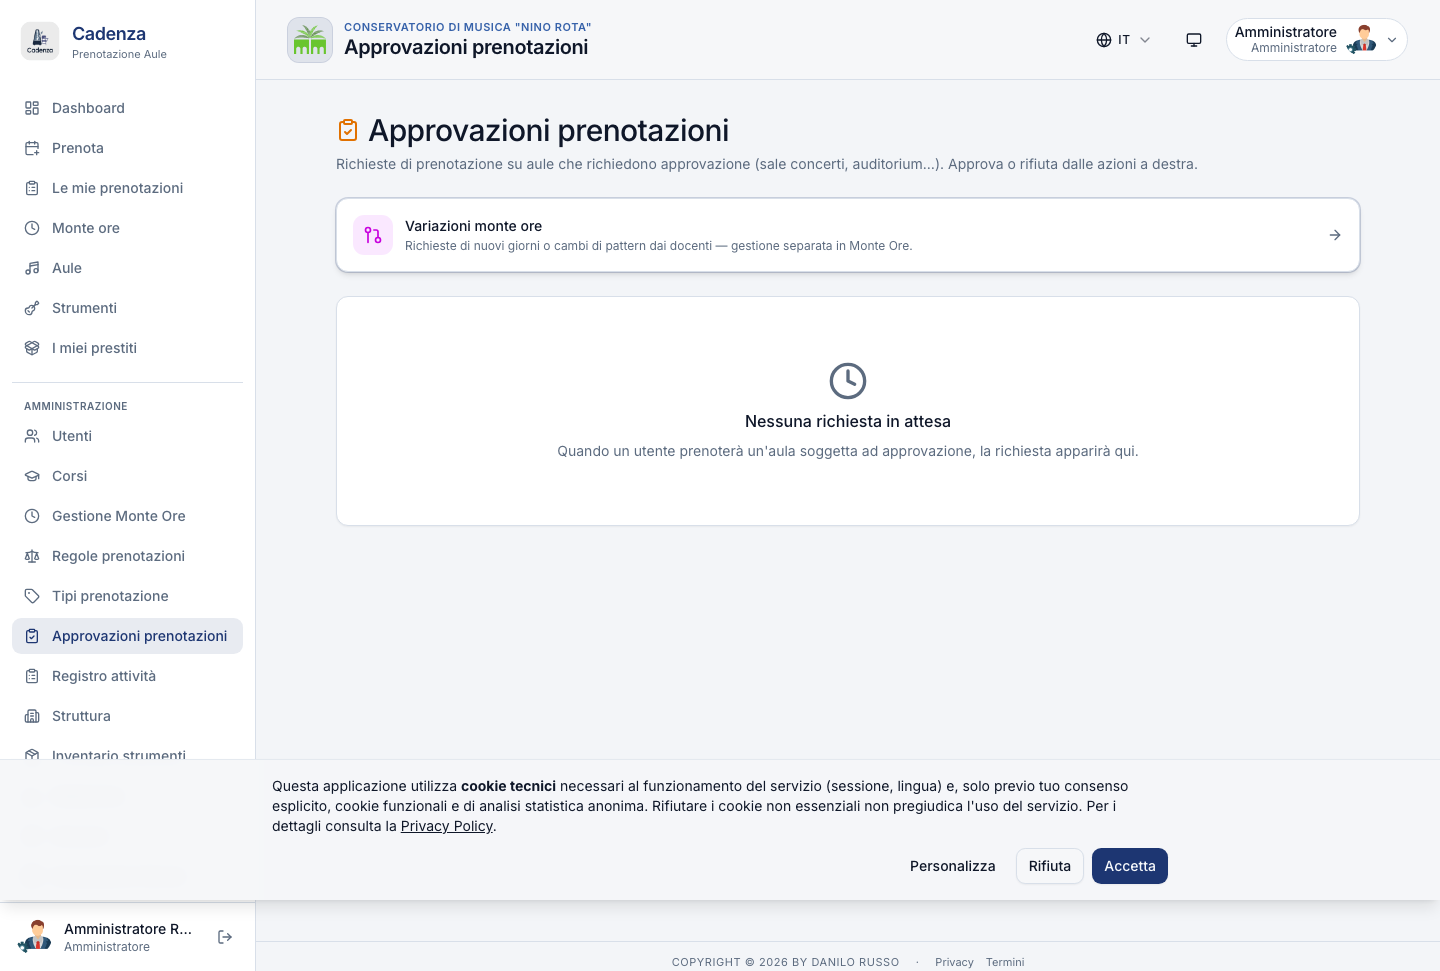
\includegraphics[width=0.95\linewidth]{screenshots/approvals-overview.png}\caption*{Pagina Approvazioni — coda richieste pending + card "Variazioni Monte Ore" con badge}\end{figure}

Qui finiscono:

\begin{itemize}
  \item prenotazioni su aule che richiedono approvazione (sale concerti, auditorium)
  \item prenotazioni di utenti il cui ruolo richiede approvazione (es. studenti in periodo di prova)
  \item prenotazioni che violano un'eccezione "approva-prima" (rara)
\end{itemize}

Per ogni richiesta vedi: utente, ruolo, aula, edificio, data/ora, durata, motivo. I bottoni sono \textbf{\checkmark{} Approva} (la prenotazione diventa confermata e va nel calendario) e \textbf{\texttimes{} Rifiuta} (apre un dialog con la textarea "Motivo del rifiuto" --- il messaggio arriva via email all'utente).

In testa alla pagina compare anche una card-link a \textbf{"Variazioni Monte Ore"} con un badge contatore \texttt{N in sospeso}: ti porta a \texttt{/admin/monte-ore?tab=amendments}. Si aggiorna automaticamente ogni 60 secondi.

\subsection{7.2 Registro attività \textbf{[!]}}


URL: \texttt{/admin/activity-log}

\begin{figure}[H]\centering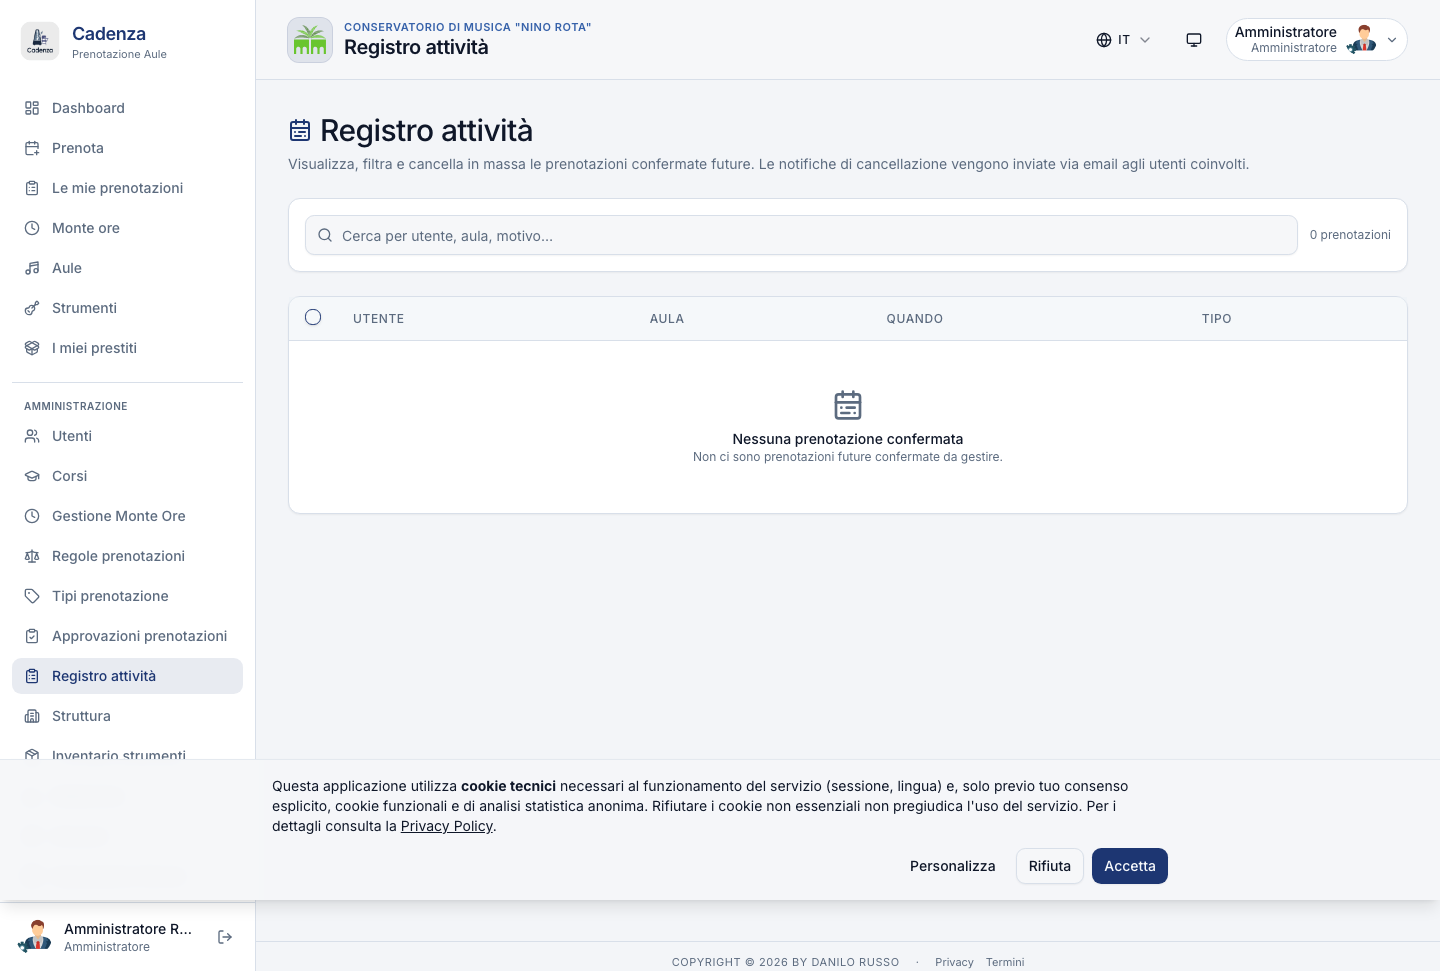
\includegraphics[width=0.95\linewidth]{screenshots/activity-log-overview.png}\caption*{Registro attività — tabella prenotazioni future con bulk-cancel e scambio aula}\end{figure}

\begin{quote}
Questa è la pagina che usi quando devi \textbf{intervenire su prenotazioni già confermate}: cancellarne molte d'un colpo (chiusura last-minute) o \textbf{scambiare} aula/orario fra due prenotazioni.
\end{quote}

Mostra solo le prenotazioni \textbf{confermate e future}. La barra di ricerca cerca su nome, cognome, email, aula, edificio e motivo.

Le colonne sono: utente, aula, quando (data + orario), tipo. Spuntando una o più righe compare la barra di selezione con il riepilogo "N prenotazioni · M utenti distinti" + i bottoni:

\begin{itemize}
  \item \textbf{$\leftrightarrow$ Scambia} --- visibile \textbf{solo} se hai selezionato esattamente 2 prenotazioni
  \item \textbf{\texttimes{} Cancella selezionate} --- sempre visibile se la selezione è \textgreater{} 0
\end{itemize}

\subsubsection{Cancellazione in blocco con motivo broadcast}


\begin{enumerate}
  \item Seleziona più prenotazioni (checkbox).
  \item Click \textbf{Cancella selezionate} $\rightarrow$ dialog con textarea \textbf{"Motivo della cancellazione"} (almeno 10 caratteri).
  \item Conferma $\rightarrow$ cancellazione in blocco + email broadcast a tutti gli utenti coinvolti, motivo incluso (senza esporre i nomi degli altri utenti).
  \item Per le prenotazioni Monte Ore lo slot collegato viene riportato attivo, salvo che cada in un'eccezione \texttt{block} attiva (vedi §6.3).
\end{enumerate}

Casi tipici: aula in ristrutturazione last-minute, sciopero, evento istituzionale.

\subsubsection{Scambio aula tra due prenotazioni}


Selezionando \textbf{esattamente 2} prenotazioni future, il bottone \textbf{"Scambia"} inverte aula e orario tra le due:

\begin{table}[H]
\centering
\small
\begin{tabularx}{\linewidth}{|X|X|}
\hline
\rowcolor{tableheader} Prima & Dopo \\
\hline
Booking A: Aula 5 · 10:00--12:00 & Booking A: Aula 8 · 14:00--15:00 \\
\hline
Booking B: Aula 8 · 14:00--15:00 & Booking B: Aula 5 · 10:00--12:00 \\
\hline
\end{tabularx}
\end{table}


Lo scambio avviene in modo \textbf{atomico} (o riesce su entrambe o non tocca nulla). Se nel frattempo qualcun altro è "entrato in mezzo" prenotando una delle aule, l'operazione viene annullata e ritenti.

\subsection{7.3 Bookings page}


URL: \texttt{/admin/bookings} --- alias deprecato di \texttt{/admin/activity-log}. Mantenuto solo perché qualcuno ha il bookmark; usa la pagina \textbf{Registro attività} per i nuovi flussi.

\begin{figure}[H]\centering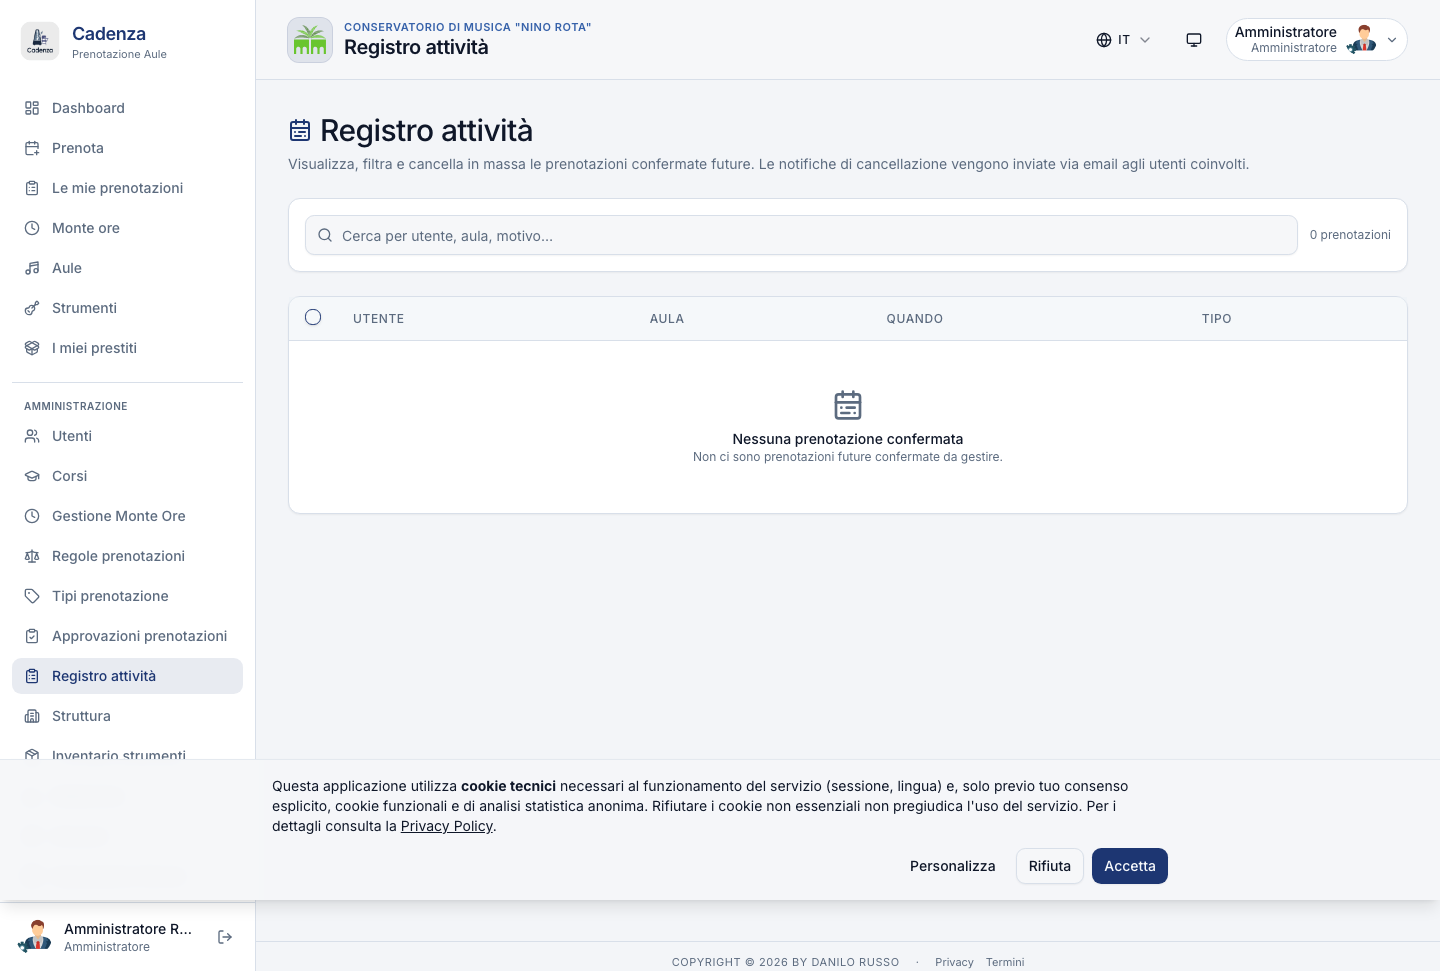
\includegraphics[width=0.95\linewidth]{screenshots/bookings-overview.png}\caption*{Pagina Bookings (alias) — stessa tabella del Registro attività}\end{figure}

\medskip\hrule\medskip

\section{8. \textbf{[!]} Gestione Monte Ore}


URL: \texttt{/admin/monte-ore}

\begin{quote}
\textbf{Cos'è}: il "Monte Ore" è il \textbf{piano annuale di insegnamento} del docente del Conservatorio italiano. Contrattualmente il docente di ruolo deve garantire \textbf{almeno 324 ore annue} di didattica, distribuite in non meno di 2 e non più di 4 giorni a settimana, in una finestra di insegnamento definita (di solito ottobre$\rightarrow$giugno). I docenti \textbf{a contratto orario} (precari, supplenti, part-time, collaboratori) hanno invece soglie individuali (tipicamente 30-200h) --- vedi §8.10. Cadenza è \textbf{il primo software italiano} che digitalizza completamente questo flusso contrattuale.
\end{quote}

\begin{figure}[H]\centering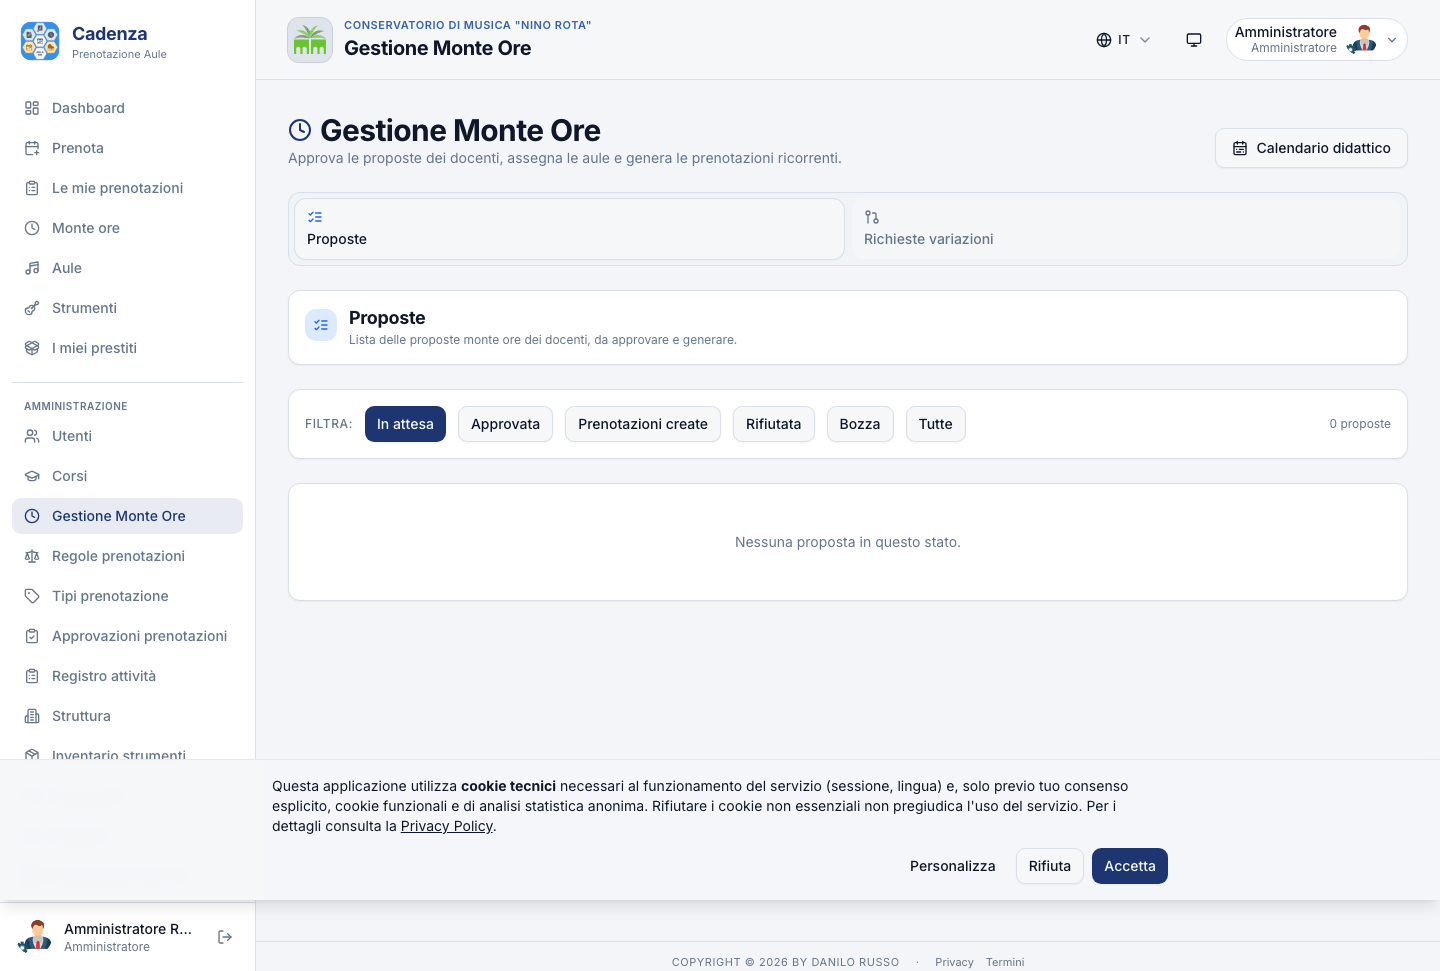
\includegraphics[width=0.95\linewidth]{screenshots/monteore-overview.png}\caption*{Pagina Gestione Monte Ore — vista lista proposte}\end{figure}

\subsection{8.1 Layout della pagina}


Pagina con \textbf{3 macro-tab card}:

\begin{itemize}
  \item \textbf{Proposte} --- coda proposte da approvare/generare
  \item \textbf{Richieste variazioni} --- variazioni post-approvazione, badge contatore in sospeso
  \item \textbf{Tipologie docenti} --- gestione tipi contratto e impatto sull'override individuale
\end{itemize}

\begin{figure}[H]\centering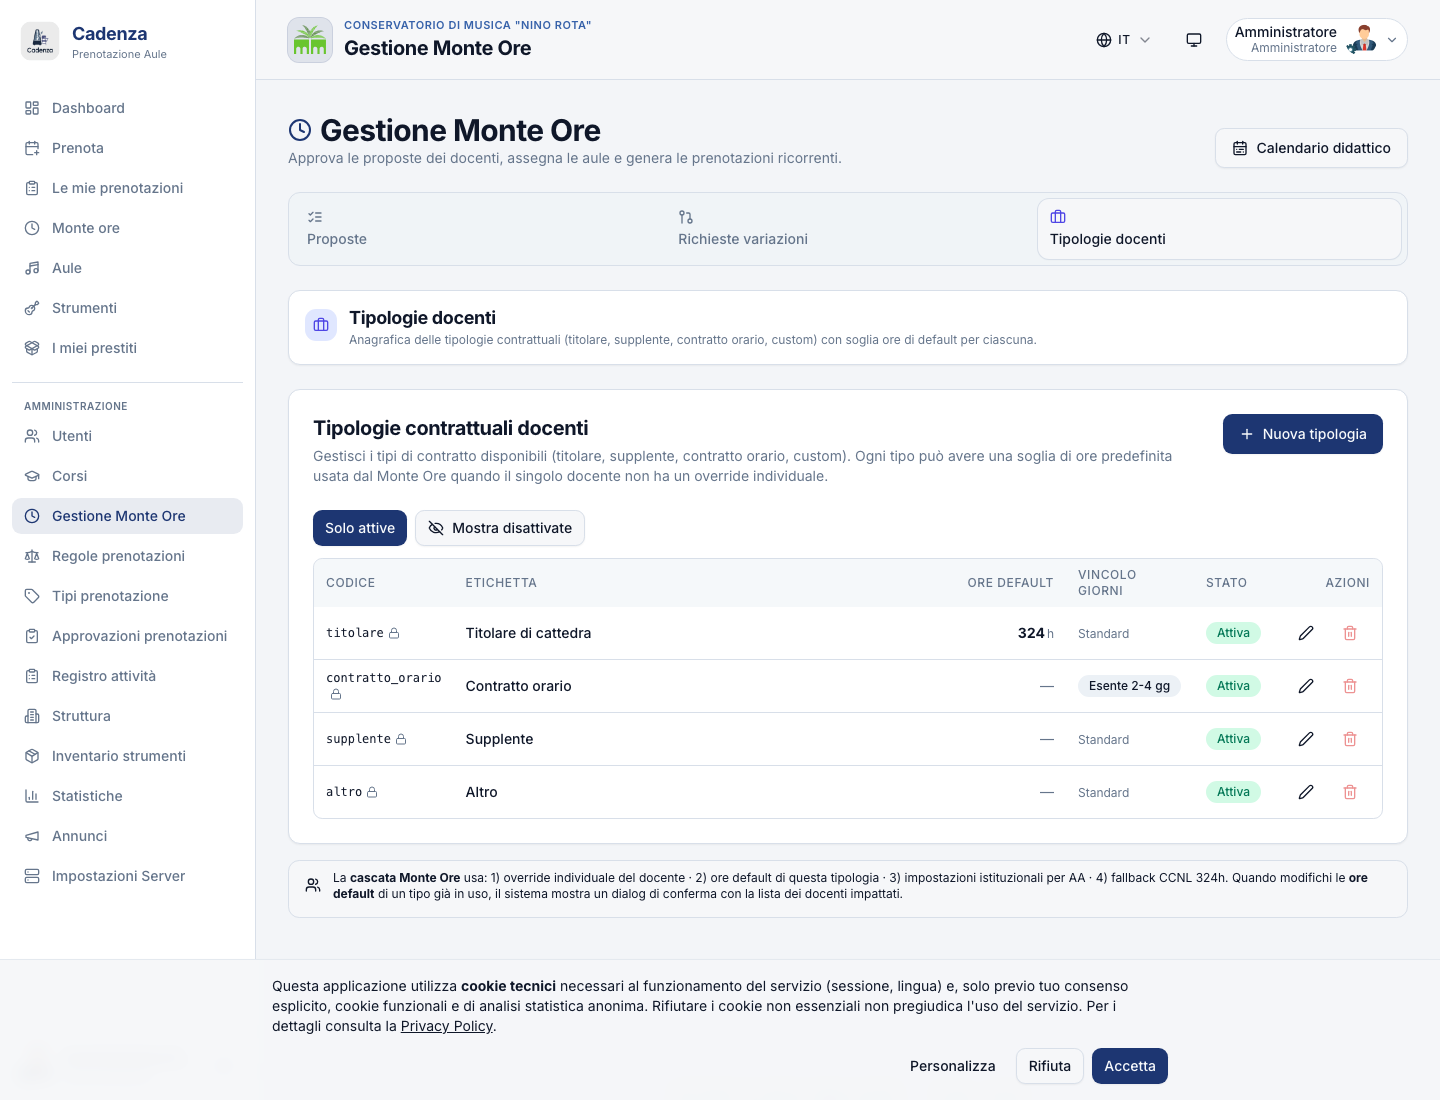
\includegraphics[width=0.95\linewidth]{screenshots/admin-monteore-contract-types.png}\caption*{Tab Tipologie docenti — anagrafica contratti (titolare, supplente, contratto orario…) con soglia ore di default}\end{figure}

In header c'è il pulsante \textbf{"Calendario didattico"} che porta alla pagina di configurazione (vedi §8.3).

\subsection{8.2 Cosa contiene il Monte Ore}


Per ogni docente Cadenza memorizza:

\begin{itemize}
  \item \textbf{Settings istituzionali}: anno accademico, finestra lezioni (es. 1 ott -- 30 giu), finestra inserimento proposte (es. 15 set -- 15 ott), soglia ore (default 324), max e min giorni a settimana.
  \item \textbf{Proposta annuale del docente}: aule scelte, schedule (giorni × orari), totale ore stimato. Stati: \texttt{bozza → in attesa → approvata/rifiutata → generata}.
  \item \textbf{Schedule}: le righe della proposta (es. "Lun 14:00--17:00 in Aula 101").
  \item \textbf{Slot}: le occorrenze concrete materializzate (es. lunedì 5/10/2026 14:00--17:00). Diventano prenotazioni vere e proprie quando approvi.
  \item \textbf{Sospensioni didattiche}: festività, ferie, esami $\rightarrow$ escludono date dalla generazione degli slot.
  \item \textbf{Variazioni} (amendments): cambiamenti su una proposta già approvata.
\end{itemize}

\subsection{8.2bis Il flusso completo del Monte Ore (vista d'insieme)}


Il Monte Ore copre un intero anno accademico e attraversa \textbf{5 fasi}. Sapere in che fase sei in un dato momento ti dice cosa fare e cosa aspettarti dai docenti.

\begin{lstlisting}
  Fase 1               Fase 2                   Fase 3              Fase 4                    Fase 5
  ──────────           ──────────────           ─────────────       ───────────────────       ──────────────────
  Settings             Inserimento              Approvazione        Generazione                Variazioni
  (admin)              (docente)                (admin)             (admin)                    (docente -> admin)
  ──────────           ──────────────           ─────────────       ───────────────────       ──────────────────
  set/ott              metà set – metà ott      ott (rolling)       metà ott                   tutto l'anno
  v                    v                        v                   v                          v
  • anno accad.        • compila griglia        • esamina lista     • crea le prenotazioni    • il docente chiede
  • finestra           • aule + giorni          • approva o         • slot Monte Ore ->          una modifica
    lezioni              + orari                  rifiuta             Booking nel calendario   • admin accetta
  • finestra           • totale h vs soglia     • controlla         • email broadcast            o rifiuta
    inserimento        • submit                   contratto                                    • amendment
  • soglia 324h                                                                                  contatore (tetto
  • sospensioni                                                                                  annuo)
\end{lstlisting}

\textbf{Stati del flusso di una proposta}:

\begin{table}[H]
\centering
\small
\begin{tabularx}{\linewidth}{|X|X|X|}
\hline
\rowcolor{tableheader} Stato & Chi può cambiarlo & Cosa succede \\
\hline
\texttt{bozza} & Docente & Sta compilando, può salvare e tornare. Nessuno la vede. \\
\hline
\texttt{in attesa} & Docente $\rightarrow$ Admin & Il docente ha cliccato "Invia". Compare nella tab Proposte dell'admin. \\
\hline
\texttt{approvata} & Admin & Tutto ok dal punto di vista contrattuale. Le aule sono assegnate. Manca solo generare. \\
\hline
\texttt{rifiutata} & Admin & Il docente riceve email con motivo. La proposta torna a "bozza" se vuole rilavorarla. \\
\hline
\texttt{generata} & Admin & Le prenotazioni sono nel calendario aule. Il docente le vede in \texttt{/my-bookings}. \\
\hline
\end{tabularx}
\end{table}


\begin{quote}
\textbf{Differenza tra "approvata" e "generata"}: il primo è la \textbf{firma contrattuale} ("ok, il piano è valido"), il secondo è la \textbf{materializzazione operativa} ("ho creato 800 prenotazioni nel calendario"). Le tieni separate per poter approvare in batch e poi generare quando il calendario è davvero pronto.
\end{quote}

\subsection{8.3 Configurazione settings (admin · una volta all'anno)}


URL diretto: \texttt{/admin/monte-ore/settings}.

\begin{figure}[H]\centering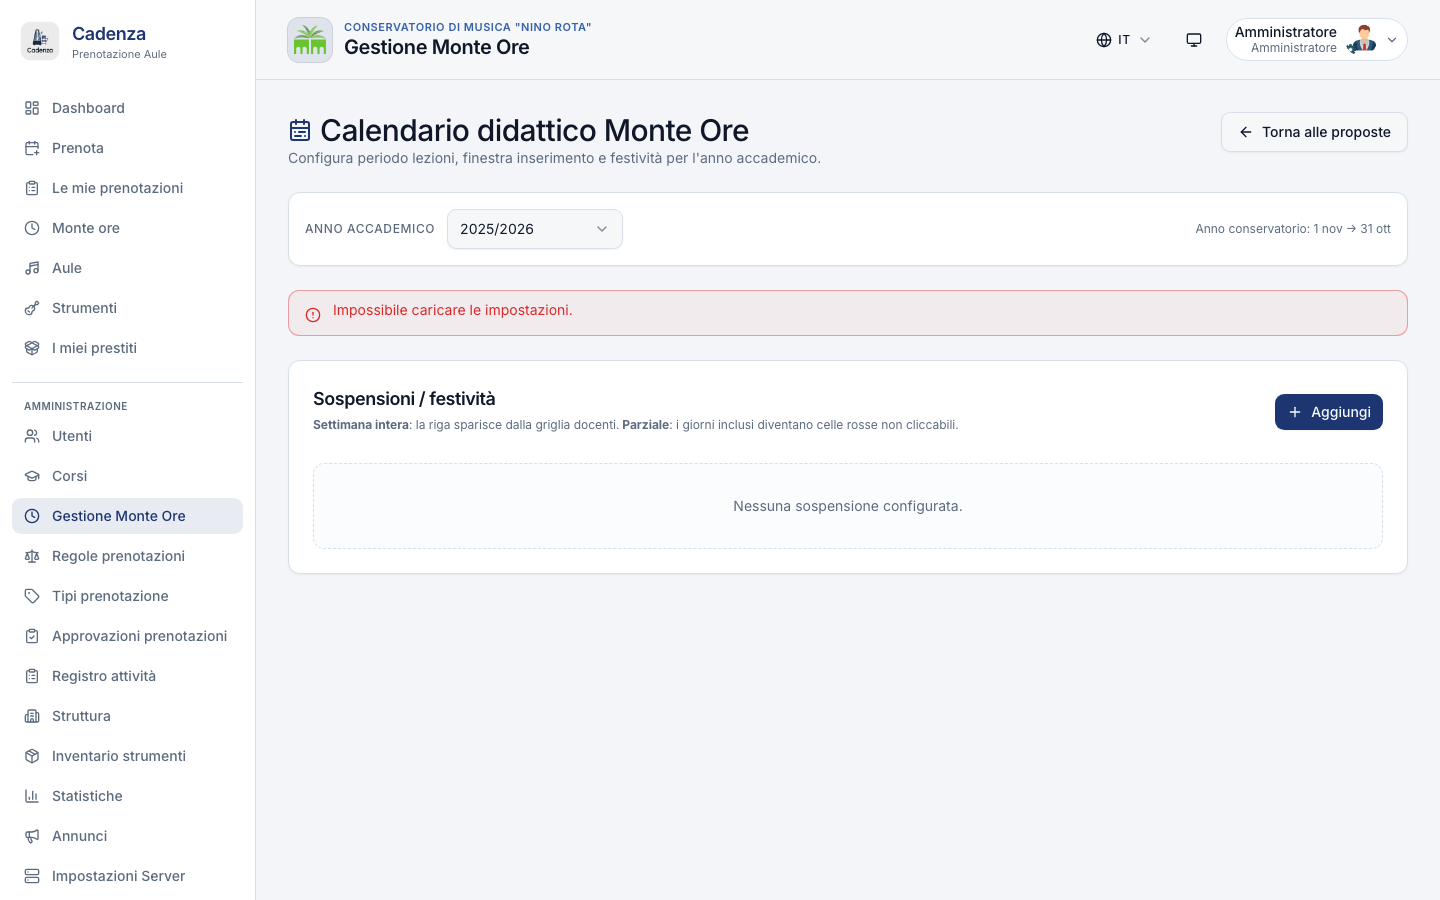
\includegraphics[width=0.95\linewidth]{screenshots/monteore-settings.png}\caption*{Tab Settings Monte Ore — soglia 324h, finestra lezioni, finestra inserimento}\end{figure}

\begin{table}[H]
\centering
\small
\begin{tabularx}{\linewidth}{|X|X|X|}
\hline
\rowcolor{tableheader} Campo & Esempio & Note \\
\hline
Anno accademico start / end & 2026-09-01 / 2027-08-31 & Periodo di riferimento contrattuale \\
\hline
Finestra lezioni start / end & 2026-10-01 / 2027-06-30 & I docenti possono pianificare lezioni solo dentro questa finestra \\
\hline
Finestra inserimento proposte & 2026-09-15 / 2026-10-15 & Periodo in cui i docenti possono compilare/sottomettere proposte \\
\hline
Soglia ore annue & 324 & Default contratto AFAM. Personalizzabile (es. 270h per docenti part-time) \\
\hline
Max richieste variazione & 3 & Tetto annuale di amendments per proposta \\
\hline
Max giorni / settimana & 4 & Vincolo CCNL \\
\hline
Min giorni / settimana & 2 & Vincolo CCNL \\
\hline
Bypass durata massima & vero & Se vero, le lezioni Monte Ore possono superare la durata max della regola del ruolo \\
\hline
\end{tabularx}
\end{table}


\begin{quote}
\textbf{Importante}: una volta che le proposte sono state approvate e generate, modificare i settings \textbf{non rigenera} automaticamente le prenotazioni. Per cambiare la finestra lezioni a metà anno servono variazioni (amendments) per ogni proposta interessata.
\end{quote}

\subsection{8.4 Sospensioni didattiche}


In coda alla pagina Settings c'è una tabella con tutte le sospensioni dell'anno accademico:

\begin{table}[H]
\centering
\small
\begin{tabularx}{\linewidth}{|X|X|}
\hline
\rowcolor{tableheader} Colonna & Contenuto \\
\hline
Nome & Es. "Vacanze di Natale" \\
\hline
Dal · Al & Range date \\
\hline
Tipo & "Settimana intera" oppure "Parziale" \\
\hline
Azioni & \textit{canc.} Elimina (con conferma) \\
\hline
\end{tabularx}
\end{table}


Form sospensione (inline): nome, data inizio/fine, tipo, e un interruttore \textbf{"Applica alle prenotazioni"} che, se attivo, crea automaticamente un'eccezione \texttt{block} nella sezione Regole.

Sospensioni tipiche da inserire all'inizio dell'anno:

\begin{itemize}
  \item Festività nazionali (1 nov, 8 dic, 25 dic, 1 gen, 6 gen, Pasqua e lunedì dell'angelo, 25 apr, 1 mag, 2 giu, 15 ago)
  \item Ferie istituzionali (es. 24 dic -- 6 gen, 1--7 settembre)
  \item Sessioni esami (es. 10--25 gen, 10--25 giu)
  \item Eventi straordinari (es. saggi pubblici dell'istituto)
\end{itemize}

Quando applichi alle prenotazioni esistenti, Cadenza marca gli slot Monte Ore futuri come "sospesi", crea un amendment automatico per ogni proposta toccata e notifica i docenti via email.

\subsection{8.5 Tab "Proposte" (vista admin)}


\begin{figure}[H]\centering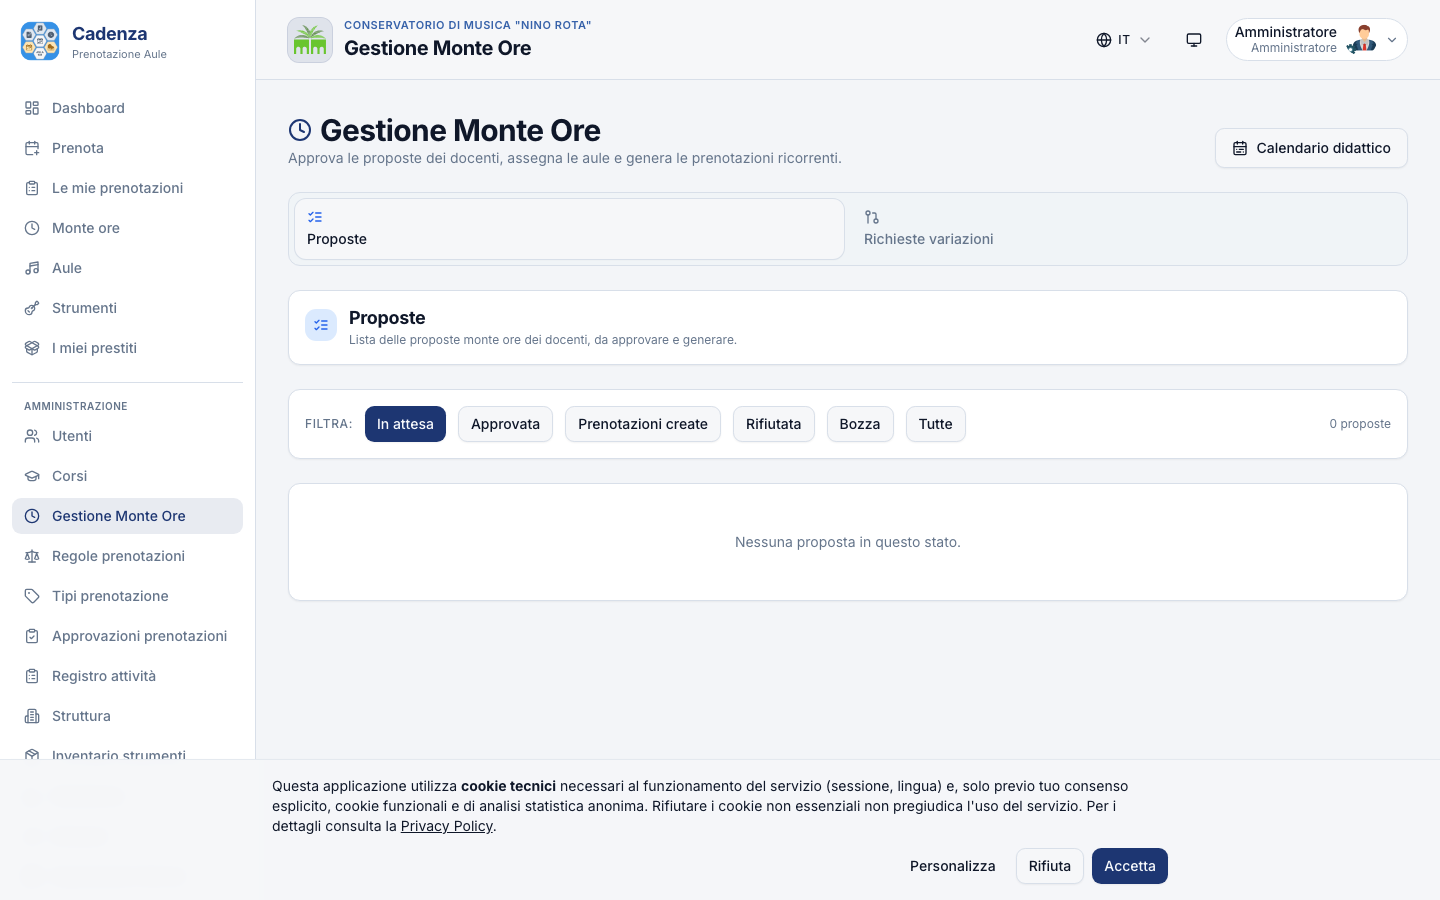
\includegraphics[width=0.95\linewidth]{screenshots/monteore-proposte.png}\caption*{Tab Proposte — filtri per stato e azione approva/rifiuta/genera}\end{figure}

Lista di tutte le proposte annuali. \textbf{Filtri per stato} in alto:

\texttt{Tutte} · \texttt{In attesa} · \texttt{Approvata} · \texttt{Generata} · \texttt{Rifiutata} · \texttt{Bozza}

Counter "\{N\} proposte" a destra. Ogni proposta è una \textbf{card cliccabile} che mostra: nome del docente, badge tipologia contratto, AA, numero di fasce, totale ore proposte vs soglia, data invio. Click su \texttt{Apri} $\rightarrow$ dialog con la tabella completa fasce orarie (giorno · orario · aula · tipo · etichetta).

Bottoni nel dialog di dettaglio:

\begin{table}[H]
\centering
\small
\begin{tabularx}{\linewidth}{|X|X|}
\hline
\rowcolor{tableheader} Stato & Bottoni \\
\hline
\texttt{In attesa} & \textbf{Approva} (verde) · \textbf{Rifiuta} (apre textarea motivo) \\
\hline
\texttt{Approvata} & \textbf{Crea prenotazioni dal monte ore} (genera gli slot e li trasforma in prenotazioni) \\
\hline
\texttt{Generata} & \textbf{Annulla generazione} (riapre la proposta --- utile se ti accorgi di un errore) \\
\hline
Sempre & Tabella fasce con \textit{mod.} Modifica / \textit{canc.} Elimina · \texttt{+ Aggiungi fascia} · \texttt{Chiudi} \\
\hline
\end{tabularx}
\end{table}


\subsubsection{Tasso di approvazione consigliato}


In media, approva direttamente le proposte dei docenti senior; usa "approva con modifiche" per spostare i nuovi docenti su aule meno richieste. Il rifiuto puro va riservato alle proposte fuori vincolo ($\geq$4 giorni/sett, \textless{}324h/anno, fuori finestra).

\subsection{8.5bis Casi guidati durante la revisione delle proposte}


Mentre esamini le proposte, ti capiteranno di sicuro questi 5 casi. Ecco cosa fare in ciascuno.

\subsubsection{Caso A --- Docente entro la soglia, aule libere}


Il caso ideale. Apri la proposta, vedi il totale ore = 324 (o sopra), nessun warning sulle aule. Click \textbf{Approva} $\rightarrow$ si arricchisce di un timestamp e passa a "Approvata". Quando hai approvato tutti i docenti del corso/sezione, torna in lista e usa \textbf{Crea prenotazioni} per generare in batch (vedi §8.7).

\subsubsection{Caso B --- Docente sotto soglia (es. 312 h vs 324)}


In dialog vedi una banda gialla "\textbf{totale 312 h vs 324 richieste}". Possibili cause:

\begin{itemize}
  \item Sospensioni dell'anno (Natale, Pasqua) sottratte automaticamente $\rightarrow$ totale "lordo" 324 ma "netto" 312.
  \item Il docente ha lasciato fuori una fascia perché in dubbio sull'aula.
\end{itemize}

Cosa fare:

\begin{enumerate}
  \item \textbf{Chiedi al docente} via mail o di persona: "ti mancano 12 ore --- vuoi aggiungere un'altra fascia?"
  \item Se sì, \textbf{rifiuta} con motivo "Manca un giorno di lezione, riapri la proposta in bozza e aggiungi una fascia di 4h × 3 settimane".
  \item Se no (es. lui ha L. 104 al 50\%), considera la \textbf{deroga individuale} (§8.10): porta la sua soglia a 162 h e riapprova.
\end{enumerate}

\subsubsection{Caso C --- Aula non assegnata su una fascia (warning icon)}


Una fascia mostra \textbf{!} "aula da assegnare". Significa che il docente ha indicato giorno + orario ma non ha potuto scegliere un'aula (era già occupata da altri docenti o non aveva permessi). Cosa fare:

\begin{enumerate}
  \item Apri la fascia (\textit{mod.} Modifica) $\rightarrow$ seleziona un'aula compatibile.
  \item Salva. Cadenza ricontrolla la disponibilità. Se OK la fascia diventa verde.
  \item Se nessuna aula libera, prova a \textbf{spostare la fascia} ad un altro slot orario (es. martedì 14-17 $\rightarrow$ giovedì 15-18) e riassegnare.
\end{enumerate}

\subsubsection{Caso D --- Conflitto al momento della generazione}


Hai cliccato \textbf{Crea prenotazioni} ma 3 slot non sono passati per overlap (un'altra prenotazione "manuale" si era infilata in quell'orario). La proposta torna in stato \textbf{"Approvata"} con un report che dice quali slot mancano.

Workflow:

\begin{enumerate}
  \item Apri la proposta $\rightarrow$ vedi "3 slot non generati" + dettaglio (data + ora + aula).
  \item Vai in \texttt{/admin/activity-log} $\rightarrow$ cerca la prenotazione conflittuale $\rightarrow$ cancella o sposta.
  \item Torna sulla proposta $\rightarrow$ click \textbf{Crea prenotazioni} di nuovo. Stavolta passa.
\end{enumerate}

\begin{quote}
\textbf{Trick}: prima di generare in massa fai un giro dell'/admin/activity-log filtrando per range di date della finestra lezioni. Se vedi prenotazioni "ad hoc" (es. studenti che si sono prenotati la prima settimana di ottobre) cancella o spostale prima.
\end{quote}

\subsubsection{Caso E --- Docente fuori vincolo (5 giorni/settimana)}


Il vincolo CCNL è 2-4 giorni/sett. Se il docente fa 5 giorni, in dialog vedi un alert rosso. Non puoi approvare. Cosa fare:

\begin{enumerate}
  \item \textbf{Rifiuta} con motivo "vincolo CCNL: max 4 giorni/sett, ridistribuisci le ore in 4 giorni".
  \item Se è un docente con \textbf{bypass del vincolo} (es. supplente part-time concordato per fare 5 giorni × 1h), imposta la deroga individuale (§8.10) $\rightarrow$ spunta "Esente dal vincolo 2-4 gg/sett" $\rightarrow$ approva.
\end{enumerate}

\subsection{8.5ter \textbf{[!]} "Richiedi modifica" --- riapertura controllata della proposta (v1.6)}


\begin{quote}
Novità di maggio 2026. Risponde al caso "la proposta è quasi corretta ma manca un dettaglio": non vuoi rifiutarla (il docente dovrebbe rifare tutto da capo) né approvarla (ci sono ancora problemi).
\end{quote}

Nel dettaglio della proposta, \textbf{finché lo stato è \texttt{In attesa} o \texttt{Approvata}}, accanto ai bottoni Approva / Rifiuta compare ora \textbf{"Richiedi modifica"} (icona \textit{(ricarica)}). Click su quel bottone apre un dialog con una textarea \textbf{"Motivazione"} (max 500 caratteri): il testo che scrivi verrà mostrato al docente in un banner rosso sulla sua pagina \texttt{/monte-ore}.

Effetti del click "Riporta in bozza":

\begin{table}[H]
\centering
\small
\begin{tabularx}{\linewidth}{|X|X|}
\hline
\rowcolor{tableheader} Stato di partenza & Cosa fa "Richiedi modifica" \\
\hline
\texttt{In attesa} & Riporta in \texttt{bozza}. Il docente può modificare e re-inviare. \\
\hline
\texttt{Approvata} & Riporta in \texttt{bozza}. Le aule assegnate restano (non vengono perse), ma la firma di approvazione viene annullata. Va re-inviata + ri-approvata. \\
\hline
\texttt{Generata} & \textbf{Non disponibile}: prima usa "Annulla generazione" per cancellare i Booking, poi "Richiedi modifica" diventa attivo. Cadenza te lo segnala con un tooltip sul bottone. \\
\hline
\end{tabularx}
\end{table}


\textbf{Differenza con "Rifiuta"}: il rifiuto è una decisione definitiva e va motivata come tale (la proposta è incompatibile con i vincoli). "Richiedi modifica" è una \textbf{collaborazione}: stai chiedendo una correzione mirata, e il docente lo capisce dal banner.

\textbf{Esempi pratici di motivazione}:

\begin{itemize}
  \item "Mancano 12 ore alla soglia 324h: aggiungi una fascia di 4h × 3 settimane."
  \item "Aula 12 non disponibile più il martedì pomeriggio (corso jazz). Spostala su Aula 5 o cambia orario."
  \item "Hai messo 5 giorni a settimana: rivedi in massimo 4 giorni come da CCNL."
  \item "Sopra soglia (340h vs 324). Ottimo, ma riduci le ore o aggiorniamo la deroga: contattaci."
\end{itemize}

Tutte le richieste di modifica passano per il \textbf{registro attività} (chi, quando, cosa). Il docente vede il banner rosso finché non re-invia.

\subsection{8.6 Tab "Richieste variazioni"}


\begin{figure}[H]\centering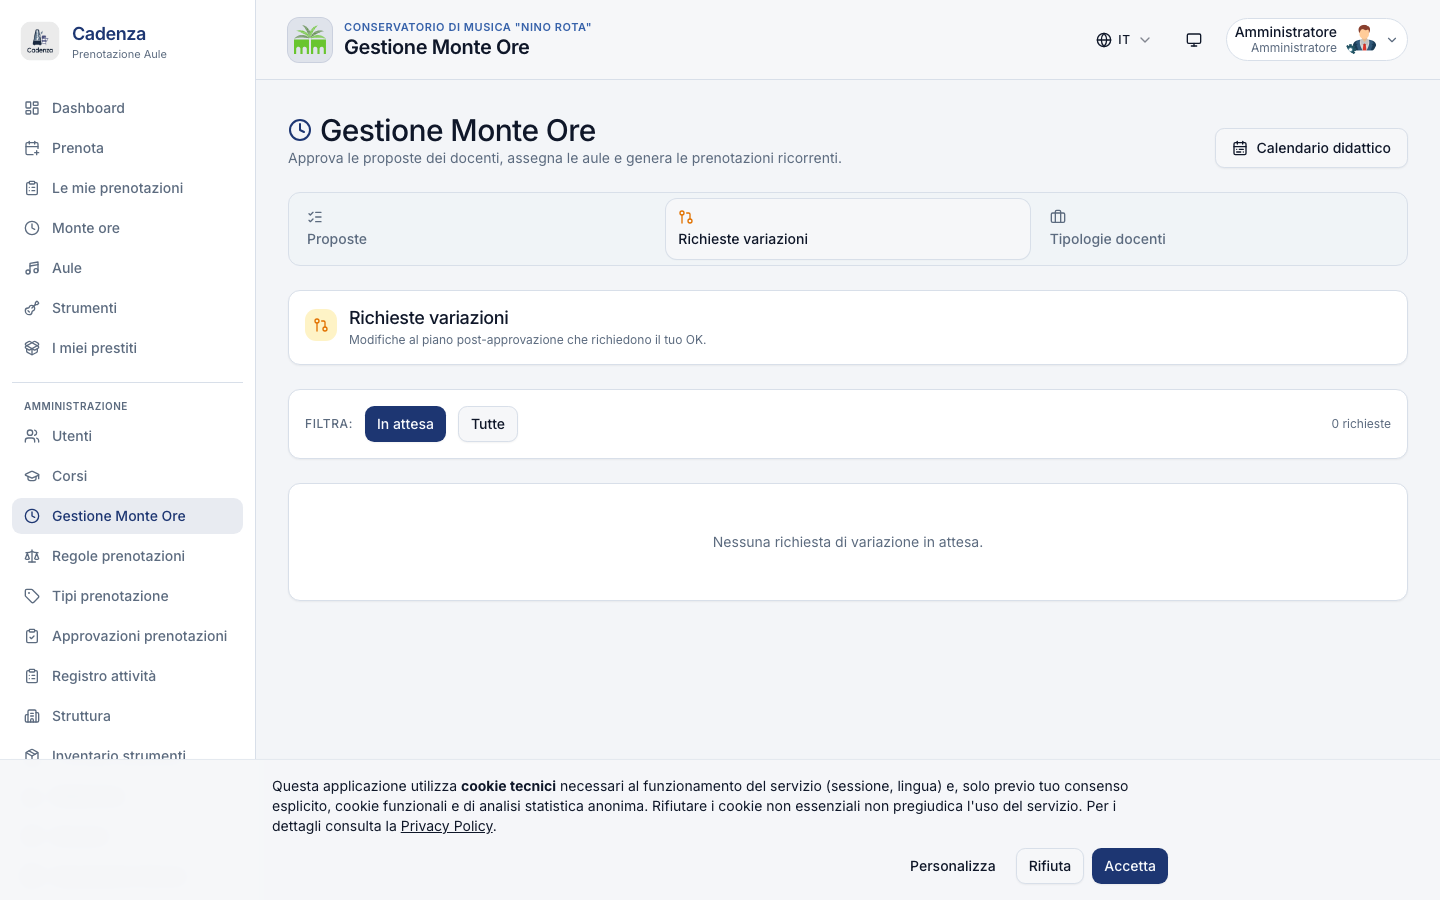
\includegraphics[width=0.95\linewidth]{screenshots/monteore-amendments.png}\caption*{Tab Richieste variazioni — coda amendment con badge pending}\end{figure}

Una volta che la proposta è approvata, il docente può chiedere di \textbf{modificare} singole occorrenze:

\begin{itemize}
  \item "La lezione di lunedì 12 ottobre la sposto a martedì 13"
  \item "Rimuovo la lezione del 5 dicembre per malattia, recupero il 7"
  \item "Cambio l'aula da 101 a 102 per i prossimi 3 mesi"
\end{itemize}

La tabella mostra: docente · AA, tipo (Disattivazione · Riattivazione · Cambio orario · Nuovo giorno · \textbf{Cambio aula} · \textbf{Spostamento}), riepilogo dello slot toccato, note del docente, stato (In attesa · Auto-approvata · Approvata · Rifiutata) e i bottoni di azione.

\subsubsection{I 6 tipi di amendment in dettaglio}


\begin{table}[H]
\centering
\small
\begin{tabularx}{\linewidth}{|X|X|X|X|}
\hline
\rowcolor{tableheader} Tipo & Cosa chiede il docente & Decisione & Effetto sul calendario quando approvi \\
\hline
\textbf{Disattivazione} & "Cancella la lezione del 12 ottobre" & \textbf{Auto} sempre (libera ore, non costa budget) & Lo slot diventa \texttt{inattivo}; la prenotazione corrispondente viene annullata \\
\hline
\textbf{Riattivazione} & "Rimetti la lezione del 12 ottobre che avevo cancellato" & \textbf{Auto} se è una cella del pattern, altrimenti pending & Lo slot torna \texttt{attivo} e Cadenza ricrea la prenotazione (se l'aula è libera) \\
\hline
\textbf{Cambio orario} & "Quella del lunedì 14:00 spostala alle 16:00" & \textbf{Auto} se la cella era nel piano originale, altrimenti pending & Lo slot mantiene la stessa data ma con i nuovi orari; il Booking viene aggiornato \\
\hline
\textbf{Nuovo giorno} & "Aggiungo una lezione il giovedì 13 ottobre, sono in ritardo con il programma" & \textbf{Pending sempre} & All'approvazione assegni l'aula $\rightarrow$ crea il nuovo slot e la prenotazione \\
\hline
\textbf{Cambio aula} \textbf{[!]} & "L'aula 12 il 22 ottobre non va, spostala in aula 5" & \textbf{Pending sempre} (l'aula è risorsa condivisa, va verificata) & Override puntuale su quella singola occorrenza; pattern e altre settimane restano invariate \\
\hline
\textbf{Spostamento} \textbf{[!]} & "Sposta la lezione del 12 ottobre al 19 ottobre" & \textbf{Auto} se sia source sia target sono nel pattern, altrimenti pending & Toggle off del source + on del target in atomico; conta come \textbf{1 sola} variazione di budget \\
\hline
\end{tabularx}
\end{table}


Per ognuno il docente scrive una \textbf{nota} facoltativa che tu vedi in chiaro al momento di approvare. Es. "spostamento per visita medica" o "recupero della classe X".

\begin{quote}
\textbf{"Auto-approvata" vs "In attesa"}: le variazioni "auto" vengono applicate dal sistema senza il tuo intervento (e segnalate nello storico). Restano comunque tracciate nel registro attività con nome del docente, slot toccato, decisione del sistema e motivazione. Le "In attesa" richiedono che tu clicchi Approva/Rifiuta nella tab. Vedi §8.6bis per la logica completa.
\end{quote}

\subsubsection{Tetto annuale di amendments}


Per evitare che la proposta venga riscritta di settimana in settimana, in \textit{Settings → Monte Ore} puoi impostare un \textbf{massimo di amendments per proposta per anno} (default: 3). Quando un docente raggiunge il tetto, vedrà un alert e non potrà più richiedere variazioni. In casi eccezionali tu admin puoi sempre \textbf{applicare modifiche manualmente} (modifica diretta della proposta) senza intaccare il contatore.

\begin{quote}
\textbf{Cosa consuma il budget}:  - \textbf{Sì}: riattivazione, cambio orario, nuovo giorno, cambio aula, spostamento (1 sola unità per spostamento, anche se è off+on di due celle) - \textbf{No}: disattivazione (libera ore, sempre lecita)
\end{quote}

\subsection{8.6bis \textbf{[!]} Spostamenti del docente --- come funzionano (v1.6)}


\begin{quote}
Da maggio 2026 il docente ha tre nuovi modi per "spostare" una lezione, oltre alla disattivazione/riattivazione di una cella. Sapere come funzionano ti aiuta a interpretare le richieste nella tab Variazioni.
\end{quote}

Sulla griglia annuale del docente, \textbf{ogni cella attiva} ha un piccolo bottone \texttt{⋮} in alto a destra. Click sul puntino apre il dialog \textbf{"Spostamento lezione"} con tre tab:

\begin{lstlisting}
  Cambia orario          Cambia aula           Sposta a…
  ─────────────          ───────────           ──────────
  Stessa data,           Stessa data e         Toggle off
  cambia start/end       orario, cambia aula   + toggle on
                                               atomico
  ─────────────          ───────────           ──────────
  AUTO se la cella       PENDING sempre        AUTO se sia
  era nel piano          (aula = risorsa       source che
  originale, altrimenti  condivisa)            target sono
  PENDING                                      nel pattern;
                                               PENDING altrim.
\end{lstlisting}

\subsubsection{Tre scenari di spostamento --- esempio guidato}


\begin{quote}
Il prof. Rossi ha una proposta approvata con pattern "Lun 14-17 in Aula 12, Mer 14-17 in Aula 12". Vediamo cosa fa il sistema quando il prof. usa ciascuna delle tre azioni.
\end{quote}

\textbf{Scenario 1 --- Cambia orario di una singola occorrenza}

Lunedì 6 novembre Rossi ha una visita medica alle 14: vorrebbe iniziare alle 16 invece che alle 14. Click \texttt{⋮} sulla cella del 6 novembre $\rightarrow$ tab \textbf{Cambia orario} $\rightarrow$ 16:00--19:00 $\rightarrow$ Salva.

\begin{itemize}
  \item Source: stesso giorno, era nel piano (\texttt{originalActive=true}) $\rightarrow$ \textbf{decisione auto-approvata}.
  \item Effetto: lo slot del 6 novembre passa a 16:00--19:00. Tutti gli altri lunedì restano alle 14:00. La prenotazione corrispondente nel calendario aule viene aggiornata.
  \item Budget: 1 variazione consumata.
\end{itemize}

\textbf{Scenario 2 --- Cambia aula per una sola settimana}

Mercoledì 8 novembre l'Aula 12 è prenotata per un concerto: Rossi sposta solo quel mercoledì in Aula 5. Click \texttt{⋮} $\rightarrow$ tab \textbf{Cambia aula} $\rightarrow$ seleziona "Aula 5 · Sede Storica" $\rightarrow$ Salva.

\begin{itemize}
  \item \textbf{Decisione pending sempre}: l'aula è risorsa condivisa, l'admin deve confermare che Aula 5 è davvero libera nel suo ruolo.
  \item Tu admin la vedi nella tab Variazioni. Apri il dialog di approvazione, controlli, \textbf{Approva}.
  \item Effetto: lo slot del 8 novembre prende \texttt{roomId = Aula 5} come override. Il pattern e tutte le altre settimane di Aula 12 restano. Il Booking corrispondente passa ad Aula 5.
  \item Budget: 1 variazione consumata all'approvazione.
\end{itemize}

\textbf{Scenario 3 --- Sposta una lezione ad un altro giorno}

Rossi vuole spostare la lezione di lunedì 13 novembre a giovedì 16 novembre. Click \texttt{⋮} sulla cella del 13/11 $\rightarrow$ tab \textbf{Sposta a\ldots{}} $\rightarrow$ seleziona "16/11 14:00--17:00" $\rightarrow$ Sposta.

\begin{itemize}
  \item Caso A: il giovedì 14:00 è una cella \textbf{inattiva del pattern} (es. il pattern aveva giovedì come opzione ma il prof. non l'aveva usato) $\rightarrow$ \textbf{auto-approvata}.
  \item Caso B: la destinazione è una cella fuori pattern $\rightarrow$ \textbf{pending}.
  \item Effetto: in atomico, lo slot del 13/11 va \texttt{inattivo} (e il Booking si cancella) + lo slot del 16/11 va \texttt{attivo} (e il Booking si crea).
  \item Budget: \textbf{1 sola variazione} consumata (non 2): è il vantaggio del "sposta a\ldots{}" rispetto a fare disattivazione + riattivazione manualmente.
\end{itemize}

\subsubsection{Cosa vedi tu admin}


Nella tab Variazioni le tipologie nuove sono etichettate:

\begin{itemize}
  \item \textbf{Cambio aula} --- sempre \texttt{In attesa}, attendono tua approvazione. Il payload include il \texttt{roomId} richiesto.
  \item \textbf{Spostamento} --- può essere \texttt{Auto-approvata} (registrata e applicata) oppure \texttt{In attesa} se la destinazione è fuori pattern.
\end{itemize}

In entrambi i casi vedi la cella sorgente e la destinazione/aula nella colonna "Cella", così puoi decidere a colpo d'occhio.

\subsubsection{Come reagire alle richieste di cambio aula}


\begin{enumerate}
  \item Apri la richiesta $\rightarrow$ vedi quale aula chiede il docente e per quale data/orario.
  \item \textbf{Controllo rapido}: nel calendario aule cerca quel slot. Se l'aula è libera, click \textbf{Approva}. Se occupata da un'altra prenotazione (es. un altro docente che ha appena prenotato), suggerisci una terza aula via "Richiedi modifica" sul singolo amendment (tab Variazioni $\rightarrow$ \texttimes{} Rifiuta con motivazione).
  \item \textbf{Cosa NON fare}: non spostare manualmente l'aula sullo \texttt{schedule} originale dal dettaglio proposta. Quello cambierebbe l'aula per \textbf{tutto l'anno}, non solo per un giorno. La richiesta di cambio aula del docente è già la modalità "puntuale" corretta.
\end{enumerate}

\subsection{8.7 Generazione slot e materializzazione prenotazioni}


Quando approvi una proposta, Cadenza:

\begin{enumerate}
  \item Calcola tutte le \textbf{occorrenze} dello schedule per ogni giorno della settimana × tutti i giorni della finestra lezioni che non sono in sospensione.
  \item Verifica che nessun'altra prenotazione collida nell'aula.
  \item Se ci sono conflitti, la proposta torna a "In attesa" con un report leggibile per la riassegnazione manuale.
  \item Crea gli slot interni e le prenotazioni corrispondenti, visibili nel calendario aule generale.
  \item Aggiorna lo status della proposta a \texttt{Generata}.
\end{enumerate}

\begin{quote}
\textbf{Tempistica}: per un docente con 6h × 4 giorni × 36 settimane (\textasciitilde{}864 occorrenze) la generazione richiede 1--3 secondi. È un'operazione tutto-o-niente: o tutto va a buon fine, o nulla viene scritto.
\end{quote}

\subsection{8.8 Calendario didattico (vista pubblica)}


Nella pagina docente \texttt{/monte-ore} c'è un bottone \textbf{"Calendario didattico"} che esporta in PDF/iCal:

\begin{itemize}
  \item per il docente: il proprio piano annuale
  \item per la Direzione (link admin): vista aggregata di tutto il monte ore del Conservatorio (incrocio aule × docenti)
\end{itemize}

Utile da inviare al sindacato o alla segreteria per i registri di insegnamento.

\subsection{8.9 Casi limite}


\begin{table}[H]
\centering
\small
\begin{tabularx}{\linewidth}{|X|X|}
\hline
\rowcolor{tableheader} Caso & Comportamento \\
\hline
Docente a contratto orario (30-200h) & Imposta deroga individuale dalla pagina Utenti $\rightarrow$ vedi §8.10 \\
\hline
Coordinatore di sezione & Nella tab Approvazioni può approvare proposte solo del proprio corso/sezione \\
\hline
Sostituto temporaneo & Crea una proposta a nome del titolare originale + amendment di "subentro" per il periodo \\
\hline
Sospensione tardiva (post-approvazione) & Inserisci la sospensione con flag "applica"; Cadenza marca gli slot come sospesi e notifica i docenti \\
\hline
Errore sistemico (es. festività dimenticata) & Inserisci la sospensione retroattiva: le prenotazioni passate restano (storico immutabile), le future vengono marcate sospese \\
\hline
\end{tabularx}
\end{table}


\subsection{8.10 \textbf{[!]} Deroga per docenti a contratto orario}


\begin{quote}
Implementata da v1.1 (aprile 2026). Risponde alla casistica del 20-40\% del corpo docente di un Conservatorio medio: contrattisti, supplenti, collaboratori, accompagnatori al pianoforte, docenti di laboratorio.
\end{quote}

\subsubsection{Perché serve}


Il modello standard di Cadenza assume \textbf{324h/anno per tutti i docenti} dell'istituto. Per i docenti a contratto orario questa soglia è errata (hanno spesso 30-200h concordate individualmente) e bloccherebbe il submit della proposta. La deroga sposta la soglia da "globale per istituto" a \textbf{"per-utente"}: ogni docente ha la sua soglia individuale + l'eventuale esenzione dal vincolo 2-4 giorni/settimana.

\subsubsection{Come configurare la deroga}


\begin{enumerate}
  \item Vai su \texttt{/admin/users} e clicca su \textbf{Modifica} del docente target.
  \item In coda al form compare la sezione \textbf{"Monte Ore --- Tipo contratto"} (visibile solo per \texttt{role=docente}).
  \item Compila: - \textbf{Tipo contratto}: la categoria informativa - \textbf{Soglia ore personalizzata}: attiva il toggle e inserisci le ore concordate (es. 60) - \textbf{Esente dal vincolo 2-4 gg/sett}: attiva se il docente concentra tutto in 1-2 giorni - \textbf{Motivazione}: obbligatoria, da intendere come riferimento contrattuale (es. "Contratto orario 60h - prot. 2026/123 del 15/09/2026")
  \item Salva. Da quel momento il submit Monte Ore di quel docente userà la soglia personalizzata.
\end{enumerate}

\begin{figure}[H]\centering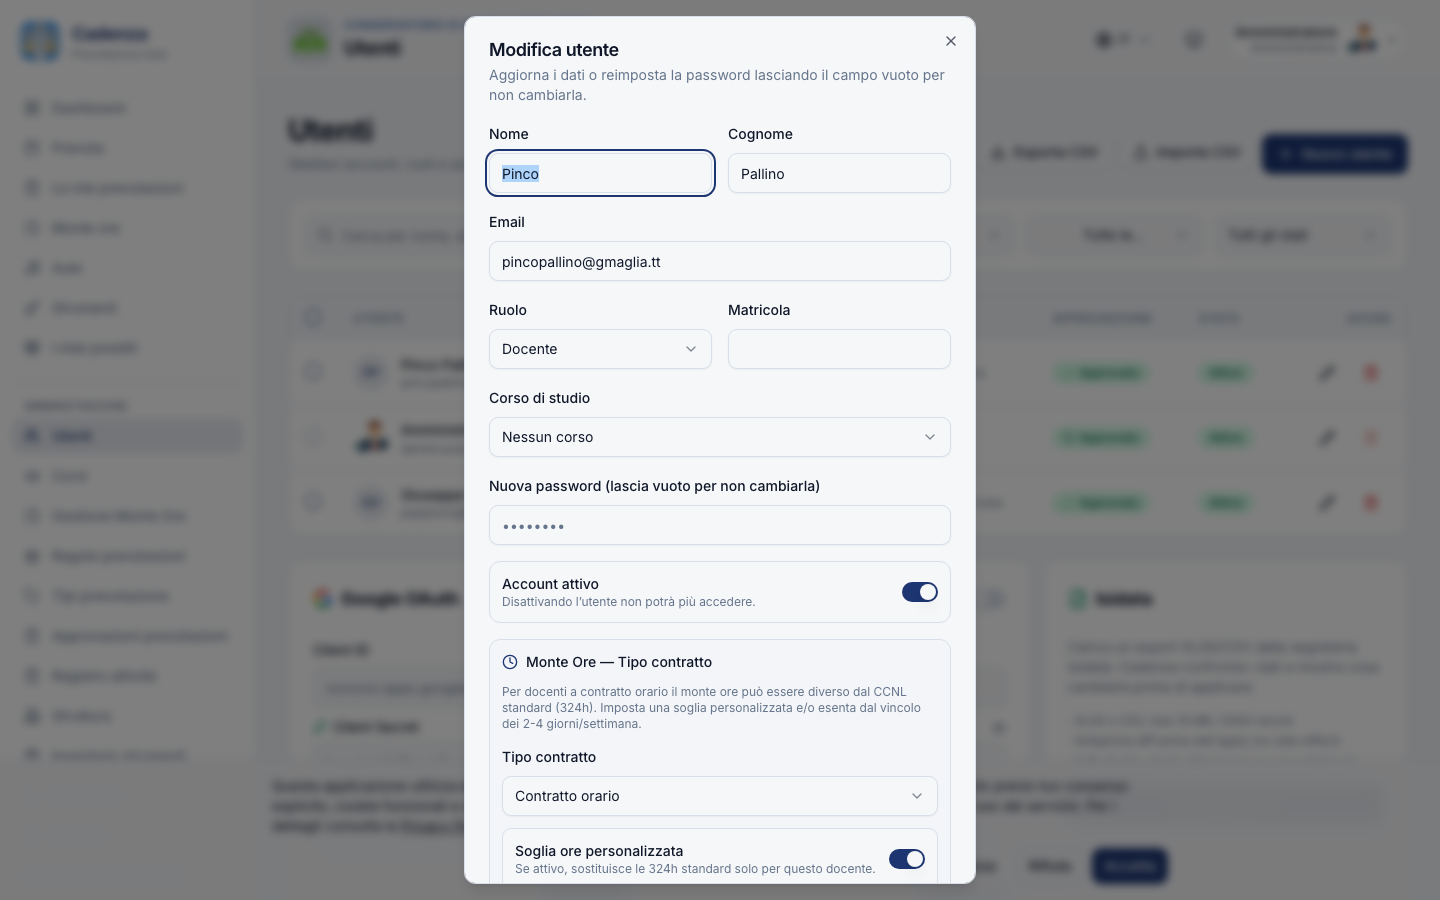
\includegraphics[width=0.95\linewidth]{screenshots/users-form-monteore-override.png}\caption*{Form override Monte Ore — sezione condizionale al ruolo docente}\end{figure}

\subsubsection{Come lo vede il docente}


Il docente con una deroga vede sulla sua pagina \texttt{/monte-ore} un banner azzurro:

\begin{lstlisting}
(i)  Soglia Monte Ore personalizzata: 60 ore/anno
   Tipo contratto: contratto orario · Vincolo 2-4 giorni/settimana: NON applicato
   Per modifiche contattare la Direzione.
\end{lstlisting}

\begin{figure}[H]\centering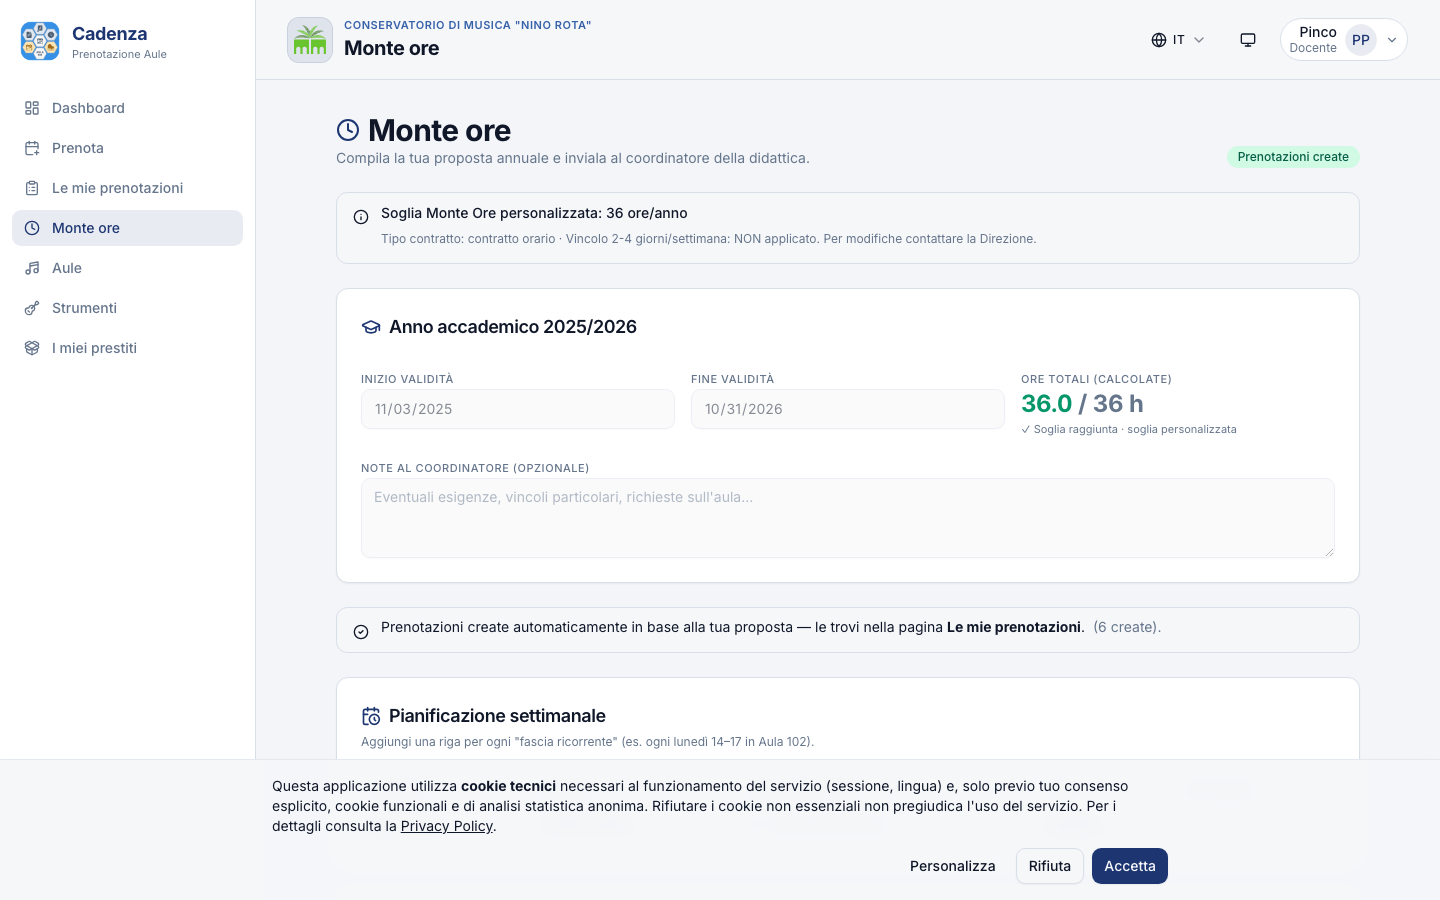
\includegraphics[width=0.95\linewidth]{screenshots/monteore-docente-banner.png}\caption*{Vista docente con banner deroga personalizzata}\end{figure}

\subsubsection{Snapshot della soglia (immutabile per proposte già inviate)}


Quando il docente fa submit, Cadenza memorizza il valore della soglia \textbf{in quel momento} dentro la proposta. Se domani rimuovi o modifichi la deroga, la proposta già inviata/approvata/generata resta valida con la soglia originale. È la "fotografia contrattuale" del momento del submit, e non si modifica retroattivamente.

\subsubsection{Esempi tipici}


\begin{table}[H]
\centering
\small
\begin{tabularx}{\linewidth}{|X|X|X|X|X|}
\hline
\rowcolor{tableheader} Categoria & Tipo contratto & Soglia & Bypass & Note \\
\hline
Titolare CCNL & titolare & --- (vuoto) & No & Default 324h dal MonteOreSettings istituzionale \\
\hline
Titolare ridotto L.104/92 & titolare & 270 & No & Riduzione per assistenza familiare \\
\hline
Supplente annuale 50\% & supplente & 162 & No & Mezzo monte ore titolare \\
\hline
Co.Co.Co. 60h annue & contratto\_orario & 60 & Sì & Tipico per coadiutori al pianoforte \\
\hline
Lab. di musica d'insieme 120h & altro & 120 & No & Da regolamento didattico \\
\hline
Accompagnatore concertistico & contratto\_orario & 30 & Sì & Concerti pubblici, monoday possibile \\
\hline
\end{tabularx}
\end{table}


\subsubsection{Conformità}


Ogni modifica della deroga viene tracciata automaticamente nel \textbf{registro attività} con: chi l'ha autorizzata, quando, valore precedente vs nuovo, motivazione. La motivazione è considerata "documento contrattuale" ai sensi della L.241/1990 §3 sulla motivazione dell'atto amministrativo. Conserva il registro per \textbf{almeno 10 anni} dalla cessazione del rapporto di lavoro (art. 2220 c.c.).

\begin{quote}
Per il dettaglio progettuale completo della deroga vedi \texttt{docs/MONTE\_ORE\_DEROGA\_CONTRATTO\_ORARIO.md}.
\end{quote}

\subsection{8.10bis \textbf{[!]} Deroga finestra di inserimento per il singolo docente (v1.6)}


\begin{quote}
Casistica tipica: la finestra Monte Ore istituzionale era 15 set -- 15 ott. È il 10 novembre e un nuovo docente (subentro per sostituzione, contratto firmato a stagione iniziata) deve presentare la sua proposta. Non vuoi riaprire la finestra globale per tutti.
\end{quote}

Nel form \textit{Modifica utente} del singolo docente, accanto agli altri campi Monte Ore, compare ora il campo:

\begin{table}[H]
\centering
\small
\begin{tabularx}{\linewidth}{|X|X|}
\hline
\rowcolor{tableheader} Campo & Significato \\
\hline
\textbf{Finestra Monte Ore aperta fino al} & Data (YYYY-MM-DD). Se valorizzata, \textbf{solo questo docente} può inviare/modificare la proposta fino a quella data, anche se la finestra globale è chiusa. \\
\hline
\end{tabularx}
\end{table}


Quando il docente arriva a \texttt{/monte-ore} e fa "Invia al coordinatore", il sistema controlla nell'ordine:

\begin{enumerate}
  \item La finestra globale (\texttt{Settings → Finestra inserimento}) è aperta?
  \item Se no, il singolo docente ha una data di deroga \texttt{≥ oggi}?
\end{enumerate}

Se entrambe le risposte sono "no", la submit viene bloccata con messaggio chiaro. Altrimenti la proposta viene inviata regolarmente.

\textbf{Quando usarla}:

\begin{itemize}
  \item Subentro contrattuale tardivo (es. nomine MIUR di novembre/gennaio)
  \item Recupero su un docente che ha avuto un problema con la procedura
  \item Anno accademico atipico (es. apertura ritardata, prolungamento)
\end{itemize}

\textbf{Quando NON usarla}:

\begin{itemize}
  \item Se tutti i docenti sono in ritardo, \textbf{riapri la finestra globale} invece (è un'azione singola e più tracciabile).
  \item Se la deroga serve per più di 2-3 docenti, valuta se la finestra istituzionale è dimensionata bene.
\end{itemize}

Tutte le deroghe sono nel registro attività con utente, valore, motivazione testuale.

\subsection{8.11 \textbf{[!]} Banner "Proposta da rivalidare" (v1.6)}


Quando l'admin modifica il \textbf{tipo contratto}, le \textbf{ore override} o l'esenzione \textbf{bypass giorni} di un docente che ha \textbf{già} una proposta in stato \texttt{In attesa}, \texttt{Approvata} o \texttt{Generata}, il sistema marca automaticamente la proposta come "da rivalidare" e mostra al docente, sulla sua pagina \texttt{/monte-ore}, un banner rosso:

\begin{lstlisting}
(!)  Proposta da rivalidare
   Variazione contratto (admin) in corso d'anno: rivedi e re-invia la proposta.
\end{lstlisting}

Il banner non blocca nulla: la proposta resta operativa fino a quando il docente la rivede. Serve come \textbf{promemoria visibile} che i presupposti della proposta sono cambiati e va data una scorsa.

\textbf{Come si svuota il flag}: alla prossima submit del docente, il banner scompare. In alternativa, se la modifica era cosmetica e non c'è bisogno di rivalidare, puoi usare "Richiedi modifica" (§8.5ter) per riportare in bozza e farsi inviare la versione aggiornata.

\begin{quote}
Tecnicamente il flag è una colonna \texttt{requiresRevalidation} sulla proposta, scritta dal hook nell'endpoint \texttt{PUT /api/users/:id/monte-ore-override}. Vedi \texttt{docs/AUDIT\_QUALITA\_PRODUZIONE.md} per il dettaglio implementativo.
\end{quote}

\medskip\hrule\medskip

\section{9. Inventario strumenti}


URL: \texttt{/admin/instruments} (con scheda \texttt{?tab=inventory|all\_loans|overdue|expiring|rules})

Pagina con \textbf{5 tab}: Inventario · Tutti i prestiti · Scaduti · In scadenza (entro 2 giorni) · Regole prestito.

\subsection{9.1 Tab "Inventario"}


\begin{figure}[H]\centering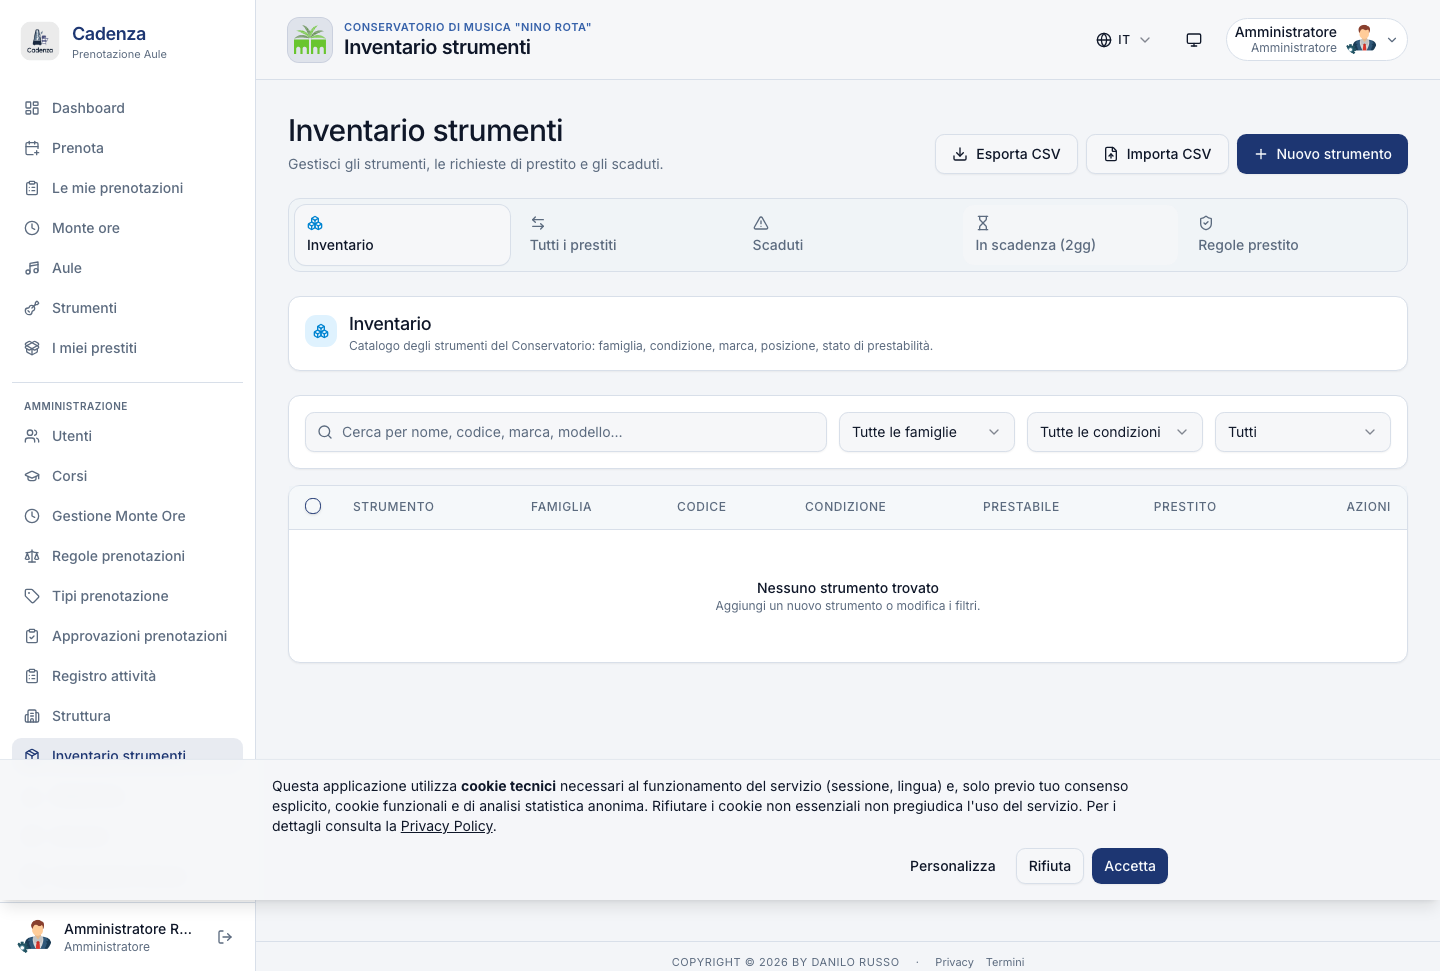
\includegraphics[width=0.95\linewidth]{screenshots/instruments-overview.png}\caption*{Tab Inventario — catalogo strumenti con filtri famiglia/condizione, foto, bulk bar}\end{figure}

In header: \textbf{Esporta CSV} · \textbf{Importa CSV} · \textbf{+ Nuovo strumento}.

I filtri permettono di restringere per \textbf{famiglia} (archi, fiati legni/ottoni, tastiere, percussioni, voce, elettronica\ldots{}), \textbf{condizione} (ottimo, buono, discreto, da\_riparare, fuori\_uso) e \textbf{prestabilità} (sì/no).

Le colonne mostrano: foto thumbnail + nome + marca/modello, famiglia, codice, condizione, "Prestabile" sì/no, stato del prestito attuale, e le azioni \textit{mod.}/\textit{canc.}.

Selezionando più righe, in basso compare la barra ambra con i bottoni: \textbf{Deseleziona}, \textbf{Abilita prestito}, \textbf{Disabilita prestito}, \textbf{Elimina}.

\subsubsection{Form Strumento}


\begin{table}[H]
\centering
\small
\begin{tabularx}{\linewidth}{|X|X|}
\hline
\rowcolor{tableheader} Campo & Descrizione \\
\hline
Nome & Es. \texttt{Violino tradizionale} \\
\hline
Codice & Codice inventario (es. \texttt{INV-0042}) \\
\hline
Famiglia & archi · fiati legni · fiati ottoni · ecc. \\
\hline
Condizione & ottimo · buono · discreto · da\_riparare · fuori\_uso \\
\hline
Marca / Modello & Stradivari · Yamaha · ecc. \\
\hline
Numero seriale & Facoltativo \\
\hline
Note & Testo libero \\
\hline
Foto & Immagine 16:9; default uno strumento generico \\
\hline
Prestabile & Disattivando, lo strumento sparisce dalla lista prestiti \\
\hline
\end{tabularx}
\end{table}


\subsection{9.2 Tab "Tutti i prestiti"}


\begin{figure}[H]\centering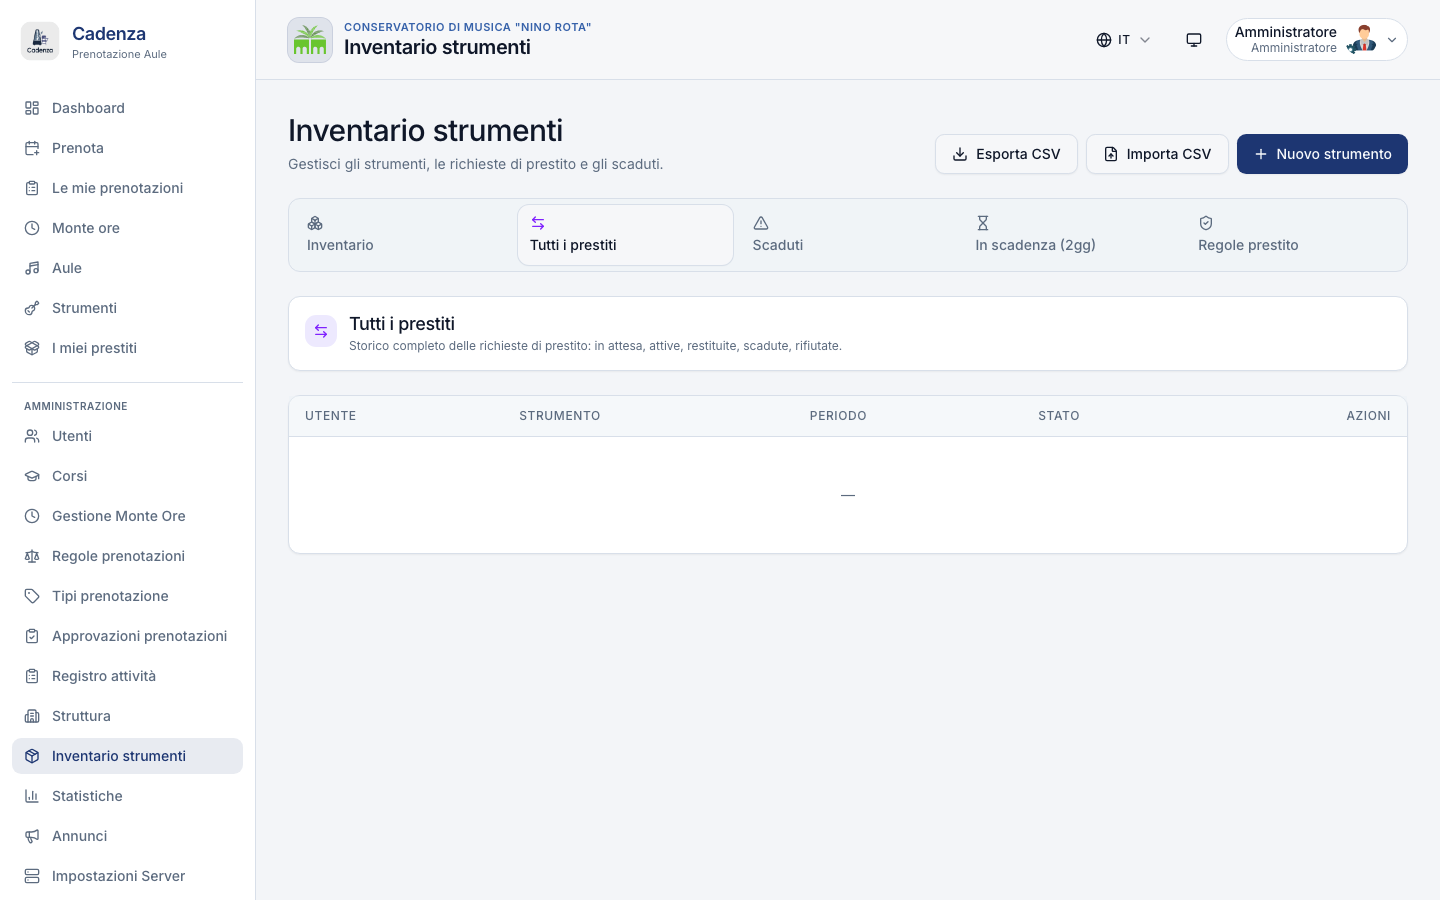
\includegraphics[width=0.95\linewidth]{screenshots/instruments-loans-all.png}\caption*{Tab Tutti i prestiti — utenti, strumento, periodo, stato e azioni PDF}\end{figure}

Tabella di tutti i prestiti con qualunque stato (\texttt{richiesto}, \texttt{attivo}, \texttt{scaduto}, \texttt{restituito}, \texttt{rifiutato}).

Colonne: utente, strumento, periodo (dal/al), stato (badge colore), azioni dipendenti dallo stato:

\begin{table}[H]
\centering
\small
\begin{tabularx}{\linewidth}{|X|X|}
\hline
\rowcolor{tableheader} Stato & Azioni disponibili \\
\hline
\texttt{richiesto} & \checkmark{} Approva (verde) · \texttimes{} Rifiuta (rosso) \\
\hline
\texttt{attivo} o \texttt{scaduto} & \textit{PDF} Stampa consegna (PDF) · \checkmark{} Forza restituzione \\
\hline
\texttt{restituito} & \textit{PDF} Stampa restituzione (PDF) \\
\hline
\end{tabularx}
\end{table}


\subsection{9.3 Tab "Scaduti" e "In scadenza"}


\begin{figure}[H]\centering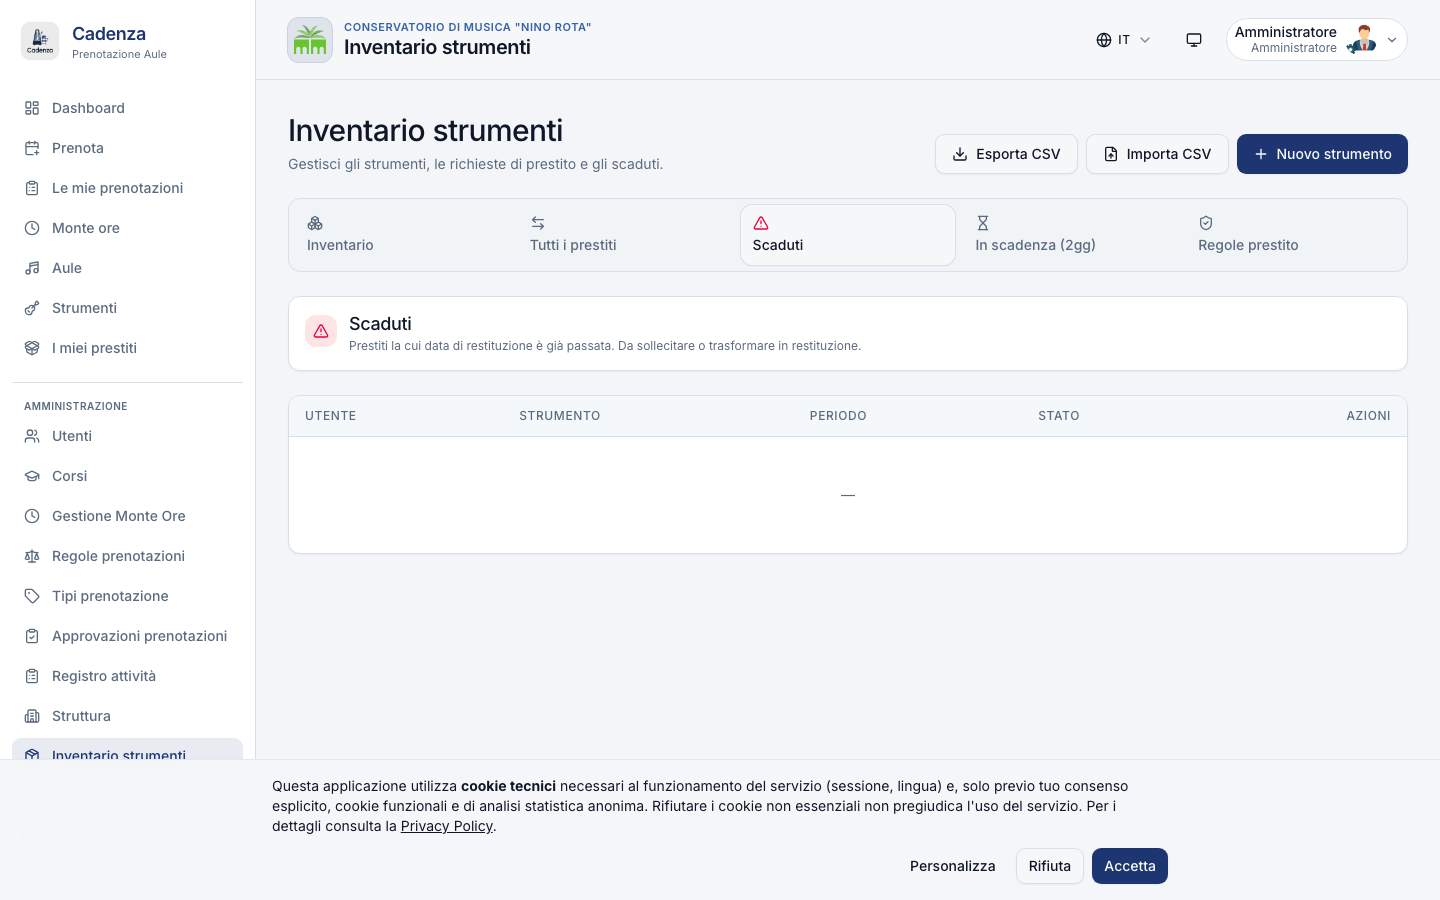
\includegraphics[width=0.95\linewidth]{screenshots/instruments-overdue.png}\caption*{Tab Scaduti — prestiti oltre la data di restituzione, con bottone Solleva}\end{figure}

Liste filtrate dei prestiti a rischio. Bottone \textbf{"Solleva"} $\rightarrow$ invia mail di reminder all'utente. Tutti i prestiti scaduti generano automaticamente reminder ogni 7 giorni.

Workflow di un prestito:

\begin{lstlisting}
richiesta -> (admin approva) -> attivo -> (utente restituisce) -> restituito
                                  v
                                scaduto (auto se oltre la data prevista)
\end{lstlisting}

Ogni cambio stato genera una mail automatica all'interessato.

\subsection{9.4 Tab "Regole prestito"}


\begin{figure}[H]\centering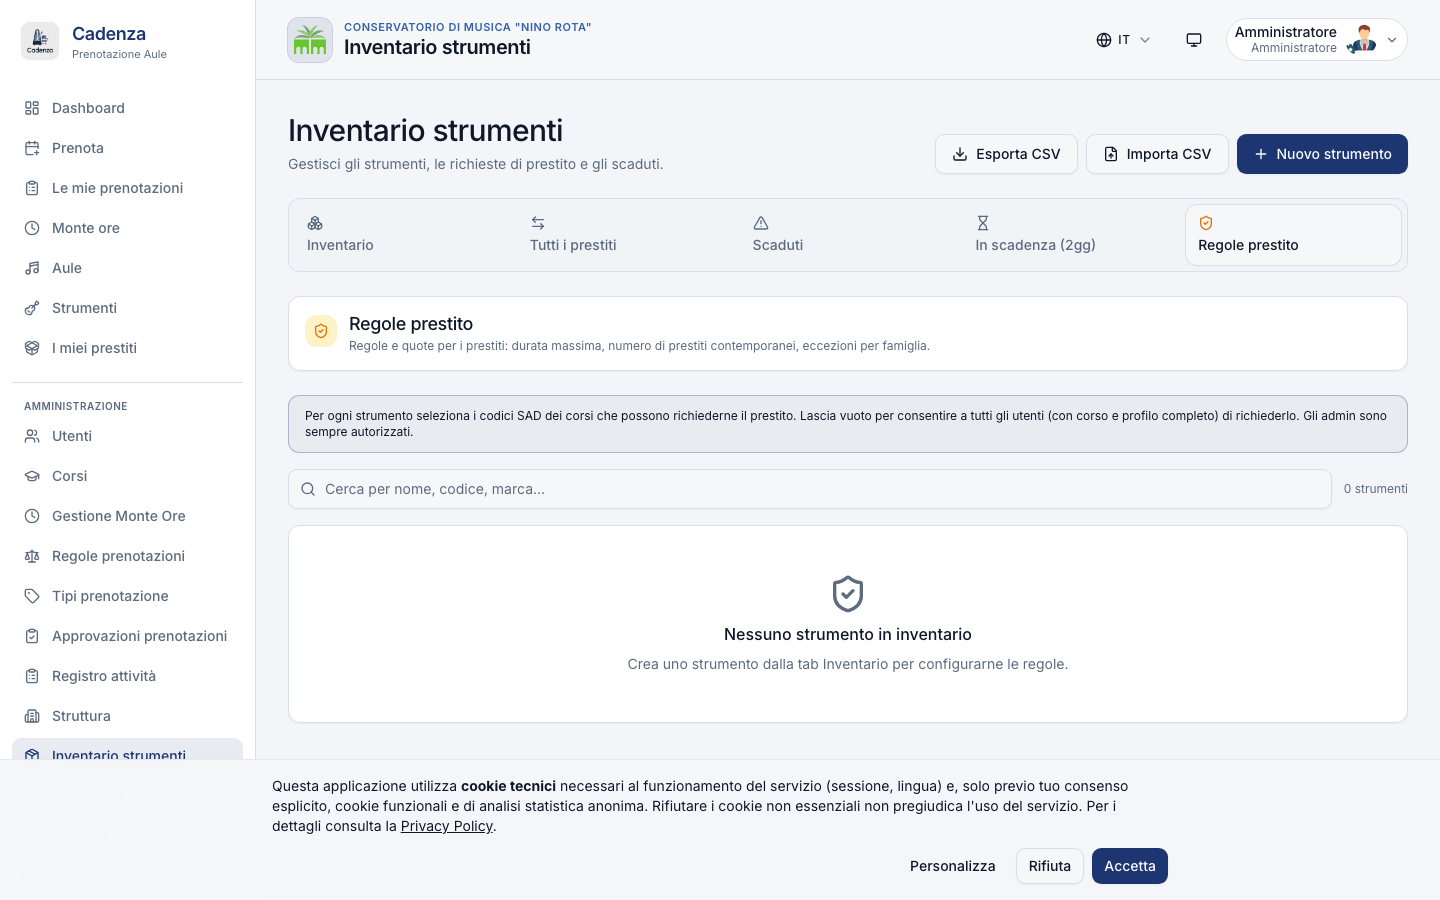
\includegraphics[width=0.95\linewidth]{screenshots/instruments-loan-rules.png}\caption*{Tab Regole prestito — mappa strumento ↔ corsi autorizzati}\end{figure}

Tabella che mappa ogni strumento ai \textbf{corsi autorizzati} a richiederlo in prestito. Per ogni riga: foto + nome + codice + famiglia + chip dei corsi (oppure "Tutto permesso").

Click \textbf{Modifica} $\rightarrow$ dialog con: ricerca corsi, bottoni \texttt{Seleziona tutto} / \texttt{Deseleziona tutto}, griglia checkbox 2 colonne dei corsi attivi.

\begin{quote}
Le \textbf{quote prestito} numeriche (max prestiti simultanei, max giorni anno) sono separate e si configurano in §6.2bis (Tab "Quote prestiti" delle Regole).
\end{quote}

\medskip\hrule\medskip

\section{10. Statistiche / Analytics}


URL: \texttt{/admin/analytics}

\begin{figure}[H]\centering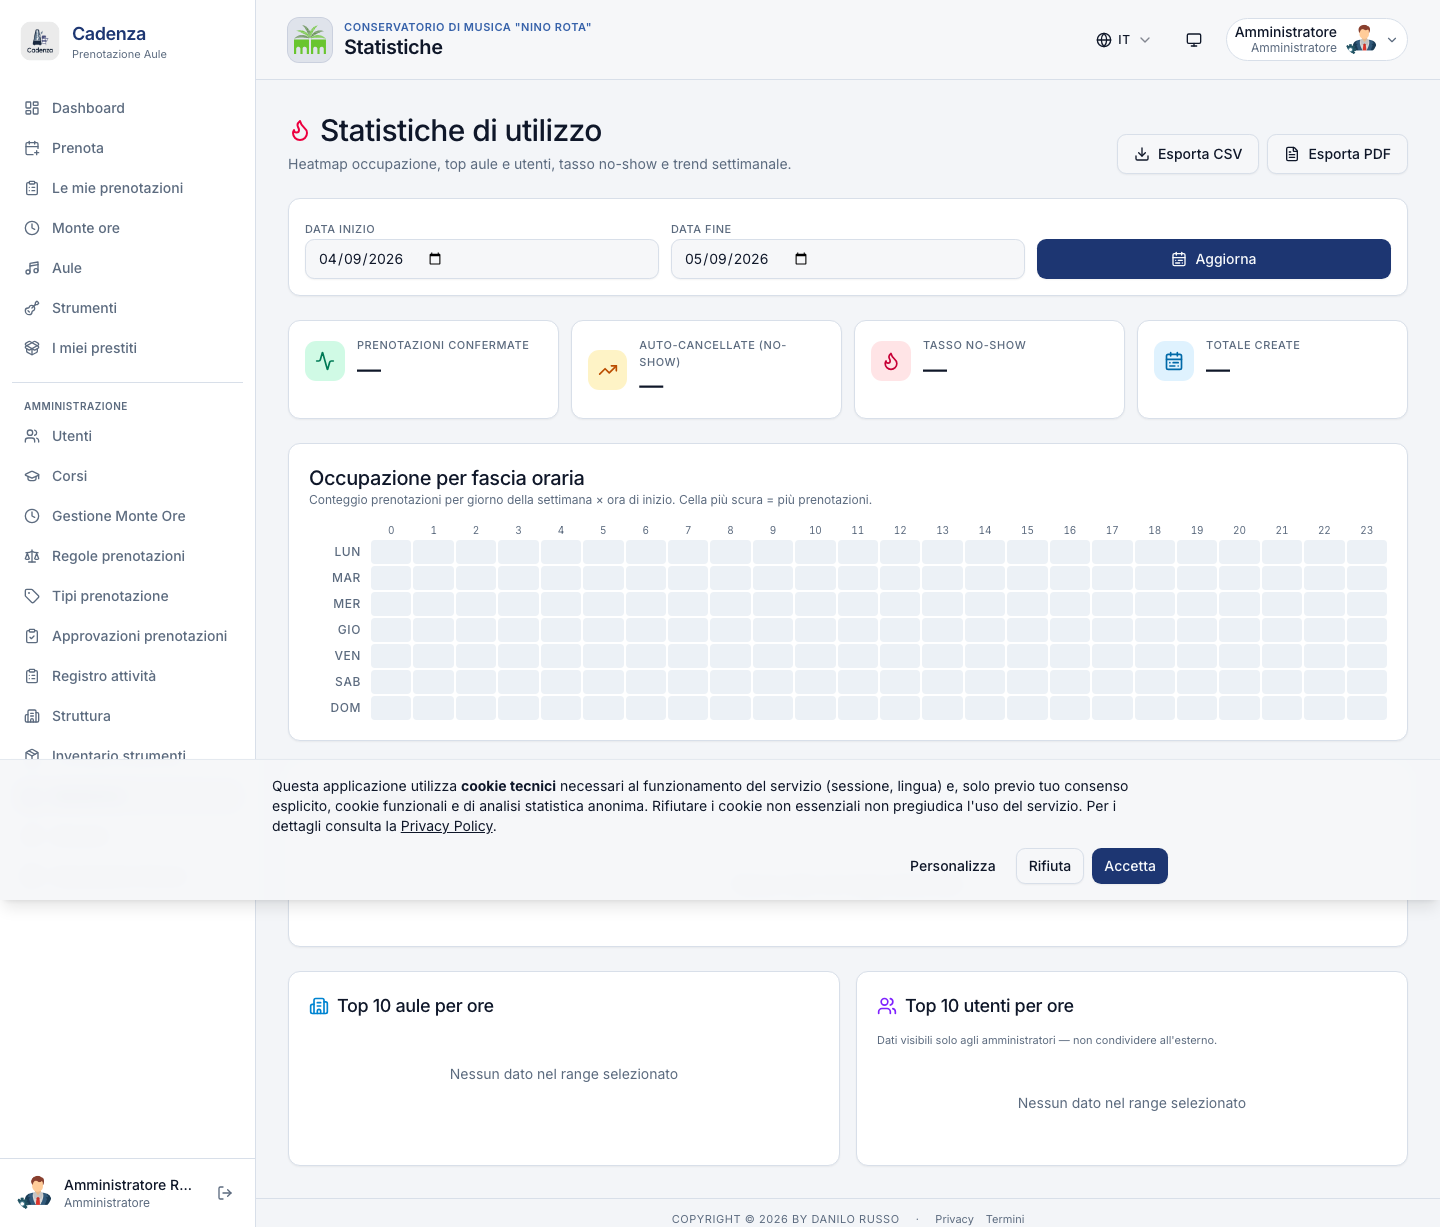
\includegraphics[width=0.95\linewidth]{screenshots/analytics-overview.png}\caption*{Pagina Analytics — KPI grid (4 card), heatmap settimanale, top aule/utenti, no-show}\end{figure}

\subsection{10.1 Layout}


In alto: bottoni \textbf{Export CSV} e \textbf{Export PDF} + filtro per data (dal--al). Sotto: 4 KPI tiles, una heatmap occupazione 7×24, una linea trend ultime 8 settimane, e i top 10 aule + top 10 utenti.

\subsection{10.2 Filtri}


\begin{table}[H]
\centering
\small
\begin{tabularx}{\linewidth}{|X|X|}
\hline
\rowcolor{tableheader} Elemento & Default \\
\hline
Date from & Oggi - 30 gg \\
\hline
Date to & Oggi \\
\hline
Apply & Refresh dati \\
\hline
\end{tabularx}
\end{table}


\subsection{10.3 KPI grid (4 card)}


\begin{itemize}
  \item \textbf{Confermate} --- prenotazioni confermate nel periodo
  \item \textbf{Auto-cancellate} --- auto-cancellate per no-show o cutoff
  \item \textbf{No-show \%} --- \texttt{auto-cancellate / (confermate + auto-cancellate) × 100}
  \item \textbf{Totale create} --- tutte le richieste, indipendentemente dallo stato finale
\end{itemize}

\subsection{10.4 Visualizzazioni}


\begin{itemize}
  \item \textbf{Heatmap 7×24}: griglia giorno × ora, cella più scura = più prenotata (ti dice quando il Conservatorio è davvero pieno).
  \item \textbf{Trend ultime 8 settimane}: ore prenotate per settimana ISO.
  \item \textbf{Top 10 aule per ore}: bar chart orizzontale (le aule più richieste).
  \item \textbf{Top 10 utenti per ore} (visibile solo agli admin, non condivisibile esternamente).
\end{itemize}

\subsection{10.5 Export}


\begin{itemize}
  \item \textbf{Export CSV} --- file con i dati grezzi del periodo
  \item \textbf{Export PDF} --- formato A4 landscape, pronto da archiviare
\end{itemize}

\begin{quote}
Per la \textbf{trasparenza GDPR}: nei report esportati i dati utente nei top 10 sono anonimizzati per default. Spuntando "Includi nomi" la scelta viene tracciata nel registro attività.
\end{quote}

\medskip\hrule\medskip

\section{11. Annunci}


URL: \texttt{/admin/announcements}

\begin{figure}[H]\centering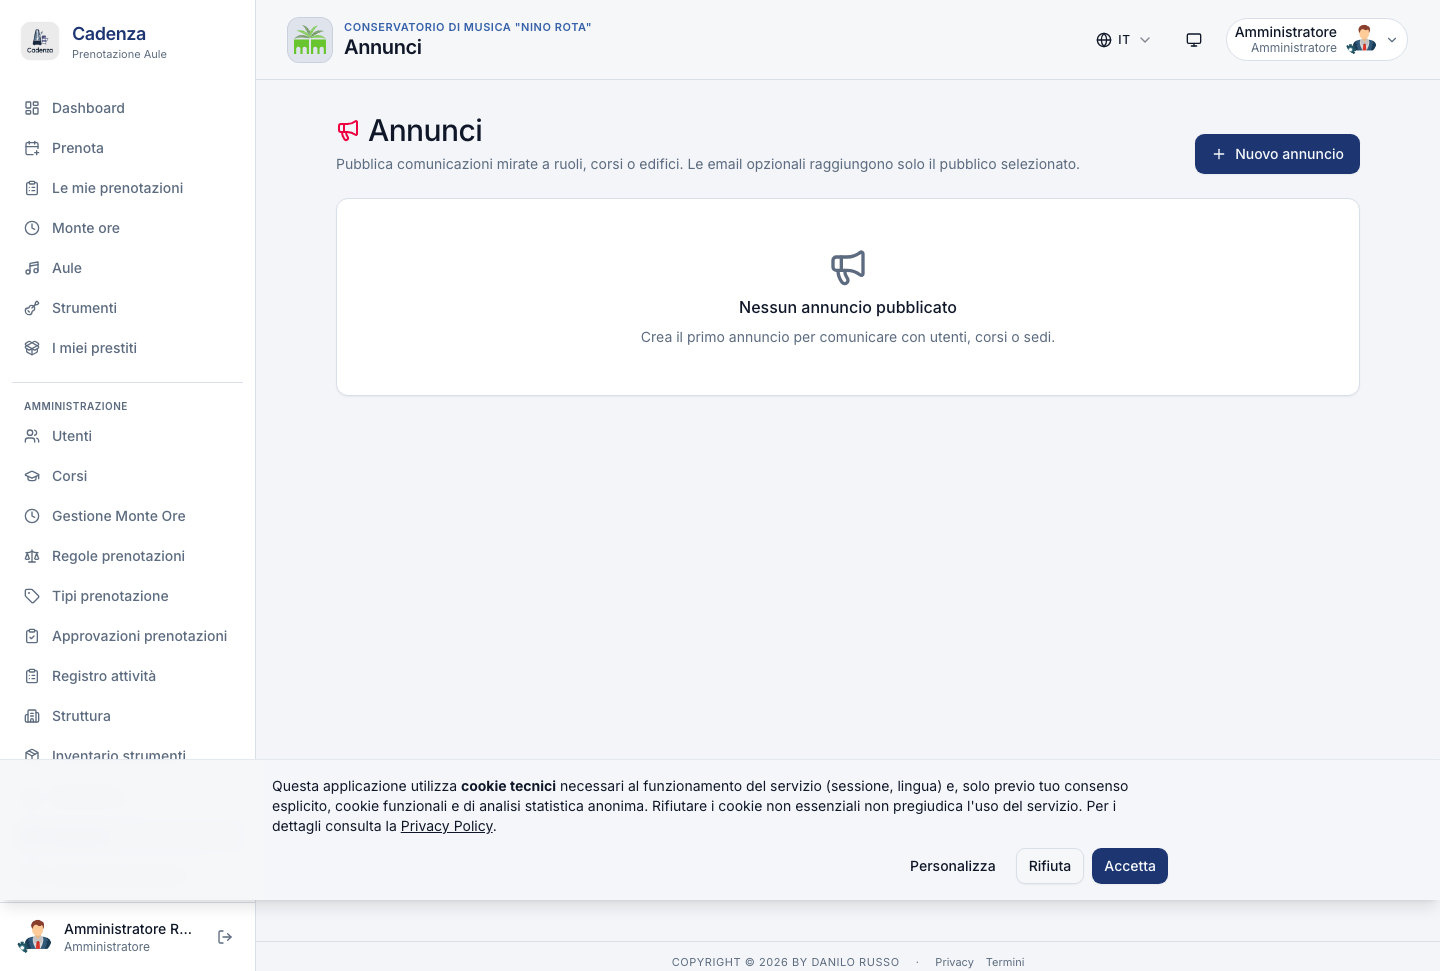
\includegraphics[width=0.95\linewidth]{screenshots/announcements-overview.png}\caption*{Pagina Annunci — griglia di card con badge audience e azioni inline}\end{figure}

In header: bottone \textbf{+ Nuovo annuncio}. Sotto, una griglia di card animate. Ogni card mostra:

\begin{itemize}
  \item Badge contestuali in alto: \textbf{Pinnato} · \textbf{Audience: tutti/role/corso/edificio} · \textbf{Inattivo} o \textbf{Scaduto} · \textbf{Email inviata}
  \item Titolo + corpo (max 2 righe troncate)
  \item Data pubblicazione e scadenza
  \item Azioni inline: \textbf{\textit{invia} Rinvia email} · \textbf{\textit{mod.} Modifica} · \textbf{\textit{canc.} Elimina}
\end{itemize}

\subsection{11.1 Form Annuncio}


\begin{table}[H]
\centering
\small
\begin{tabularx}{\linewidth}{|X|X|}
\hline
\rowcolor{tableheader} Campo & Descrizione \\
\hline
Titolo & Massimo 200 caratteri \\
\hline
Corpo & Testo lungo, supporta Markdown semplice \\
\hline
Pubblicato il & Default = adesso. Date future = bozze automatiche \\
\hline
Scadenza & Dopo questa data l'annuncio sparisce dal feed \\
\hline
Audience kind & Tutti · Per ruolo · Per corso · Per edificio \\
\hline
Audience value & Necessario se diverso da "Tutti" (dropdown ruoli/corsi/edifici) \\
\hline
Pin & L'annuncio resta sempre in cima alla lista \\
\hline
Attivo & Disattivando lo nascondi senza cancellarlo \\
\hline
Invia email & Spunta se vuoi mandare anche un'email broadcast all'audience \\
\hline
\end{tabularx}
\end{table}


\begin{quote}
\textbf{Modifica annuncio}: la modifica \textbf{non rimanda} automaticamente l'email. Se vuoi notificare di nuovo, usa l'azione \textbf{\textit{invia} Rinvia email} sulla card.
\end{quote}

\subsection{11.2 Audience targeting}


\begin{table}[H]
\centering
\small
\begin{tabularx}{\linewidth}{|X|X|X|}
\hline
\rowcolor{tableheader} Tipo & Esempio & Visibilità \\
\hline
Tutti & --- & Tutti gli utenti + display kiosk \\
\hline
Ruolo & \texttt{docente} & Solo docenti \\
\hline
Corso & \texttt{DCPL34 (Pianoforte)} & Studenti del corso indicato \\
\hline
Edificio & \texttt{Edificio centrale} & Solo display kiosk dell'edificio (non nel feed personale) \\
\hline
\end{tabularx}
\end{table}


Gli annunci \textbf{pinnati} finiscono anche nella rotazione del display kiosk pubblico nelle aule (vedi §12.7 per la configurazione globale del display).

\medskip\hrule\medskip

\section{12. Impostazioni Server}


URL: \texttt{/admin/server-settings}

\subsection{12.0 Hub di navigazione macro/sub-tab}


La pagina è un \textbf{hub} organizzato in macro-tab in alto + sub-tab quando la macro è "Servizi":

\begin{lstlisting}
Impostazioni Server
├─ Servizi   ├─ Mail · Mail Outbox · Messaging · Backups · Export Excel
├─ Aspetto
├─ QR Codes
├─ Display
├─ Audit Log
└─ Moduli
\end{lstlisting}

\begin{table}[H]
\centering
\small
\begin{tabularx}{\linewidth}{|X|X|X|}
\hline
\rowcolor{tableheader} Macro & Sub-tab & Sezione manuale \\
\hline
Servizi & Mail · Mail Outbox · Messaging · Backups · Export Excel & §12.1 · §12.2 · §12.3 · §12.4 · §12.4bis \\
\hline
Aspetto & (nessuna sub) & §12.5 \\
\hline
QR Codes & (nessuna sub) & §12.6 \\
\hline
Display & (nessuna sub) & §12.7 \\
\hline
Audit Log & (nessuna sub) & §12.8 \\
\hline
Moduli & (nessuna sub) & §12.9 \\
\hline
\end{tabularx}
\end{table}


\subsection{12.1 Servizi $\rightarrow$ Mail (SMTP)}


\begin{figure}[H]\centering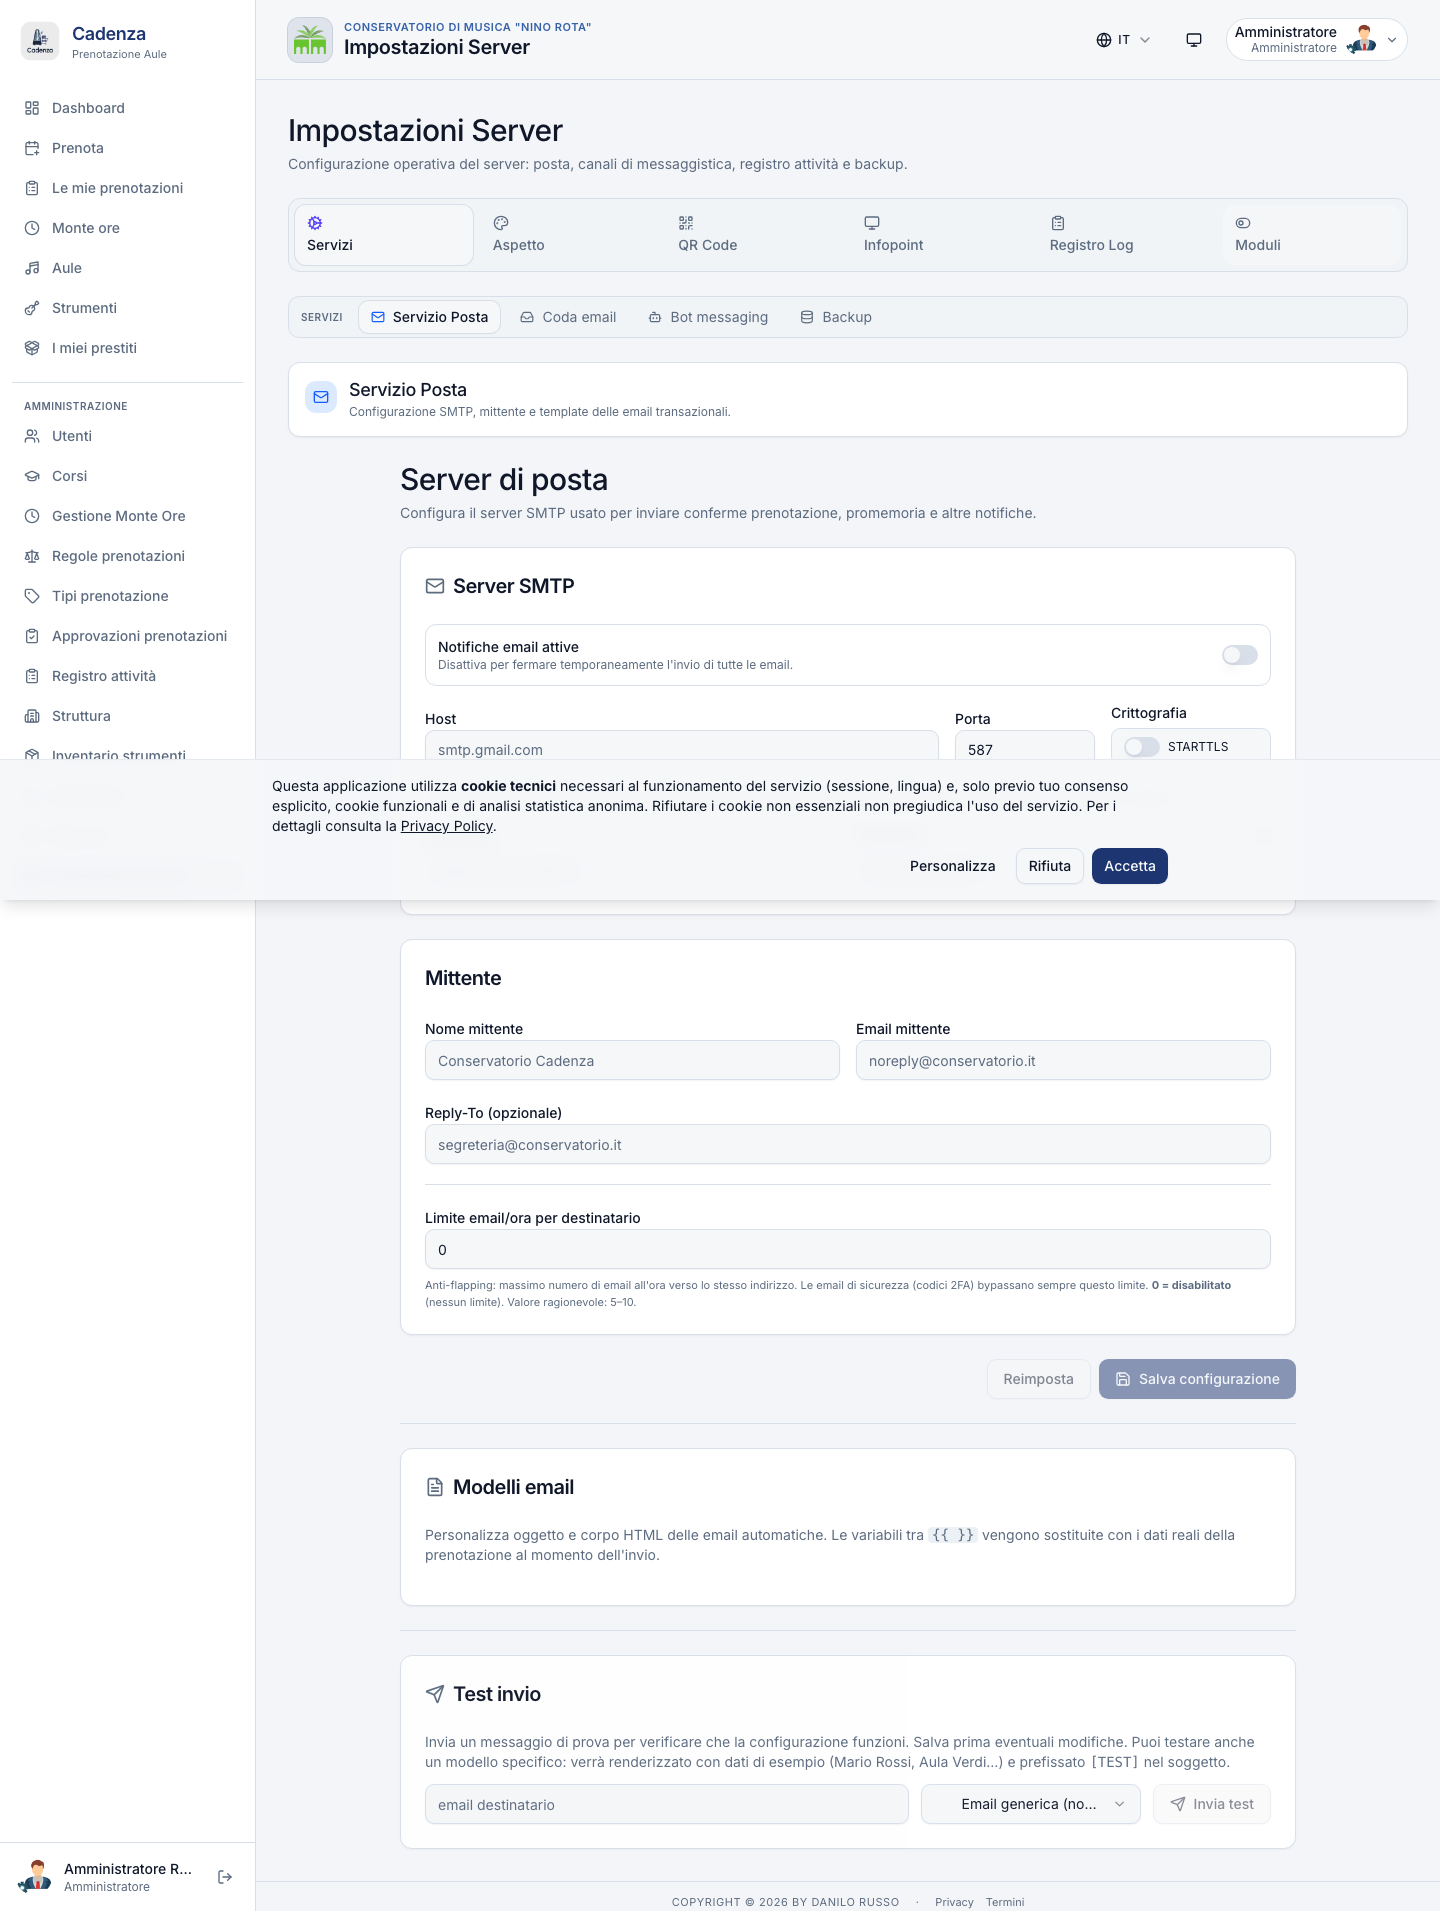
\includegraphics[width=0.95\linewidth]{screenshots/server-settings-servizi-mail.png}\caption*{Sotto-tab Servizi → Mail}\end{figure}

In alto compare il badge di stato della configurazione: \textbf{Configurato (DB)} · \textbf{Disabilitato} · \textbf{Non configurato}. Se sono attive variabili d'ambiente SMTP, un alert blu informa che salvare la form prenderà il loro posto.

\subsubsection{Card "Server SMTP"}


\begin{table}[H]
\centering
\small
\begin{tabularx}{\linewidth}{|X|X|}
\hline
\rowcolor{tableheader} Campo & Descrizione \\
\hline
Abilitato & Interruttore per accendere/spegnere l'invio mail \\
\hline
Host & Es. \texttt{smtp.gmail.com} \\
\hline
Porta & Tipicamente 465 (TLS) o 587 (STARTTLS) \\
\hline
Connessione sicura (TLS) & TLS implicito (porta 465) vs STARTTLS (porta 587) \\
\hline
Username & Account autenticato \\
\hline
Password & Mai pre-compilata (lascia vuoto = nessun cambio). Bottone occhio per mostrare \\
\hline
From address & Es. \texttt{noreply@conservatorio.it} \\
\hline
From name & Es. \texttt{Conservatorio · Cadenza} \\
\hline
Reply-to & Indirizzo a cui arrivano le risposte \\
\hline
Throttle per destinatario / ora & 0--1000. \texttt{0} = disabilitato. Mette un tetto al numero di mail per ora allo stesso indirizzo (anti-flapping) \\
\hline
\end{tabularx}
\end{table}


\subsubsection{Banner di aiuto}


\begin{itemize}
  \item \textbf{Mismatch porta/sicura} (ambra): porta 465 senza TLS, oppure 587/25 con TLS
  \item \textbf{Typo nell'host} (ambra): \texttt{smpt.} rilevato $\rightarrow$ suggerisce auto-correct in \texttt{smtp.}
  \item \textbf{Password salvata}: badge verde accanto al label password se è già presente nel database
\end{itemize}

\subsubsection{Card "Modelli email"}


Dropdown per selezionare un template della libreria (badge \texttt{OFF} se disabilitato) $\rightarrow$ apre l'editor con preview e bottone Salva.

\subsubsection{Card "Test invio"}


Compili destinatario e tipo email (Generica · uno specifico template), clicchi \textbf{Invia test} e vedi il risultato sotto: \textcolor{green!60!black}{\checkmark{}} verde se il messaggio è partito, \textcolor{red}{$\times$} rosso con dettaglio se ha fallito.

\subsection{12.2 Servizi $\rightarrow$ Mail Outbox}


URL legacy: \texttt{/admin/mail-outbox} (ora sub-tab di Server Settings).

\begin{figure}[H]\centering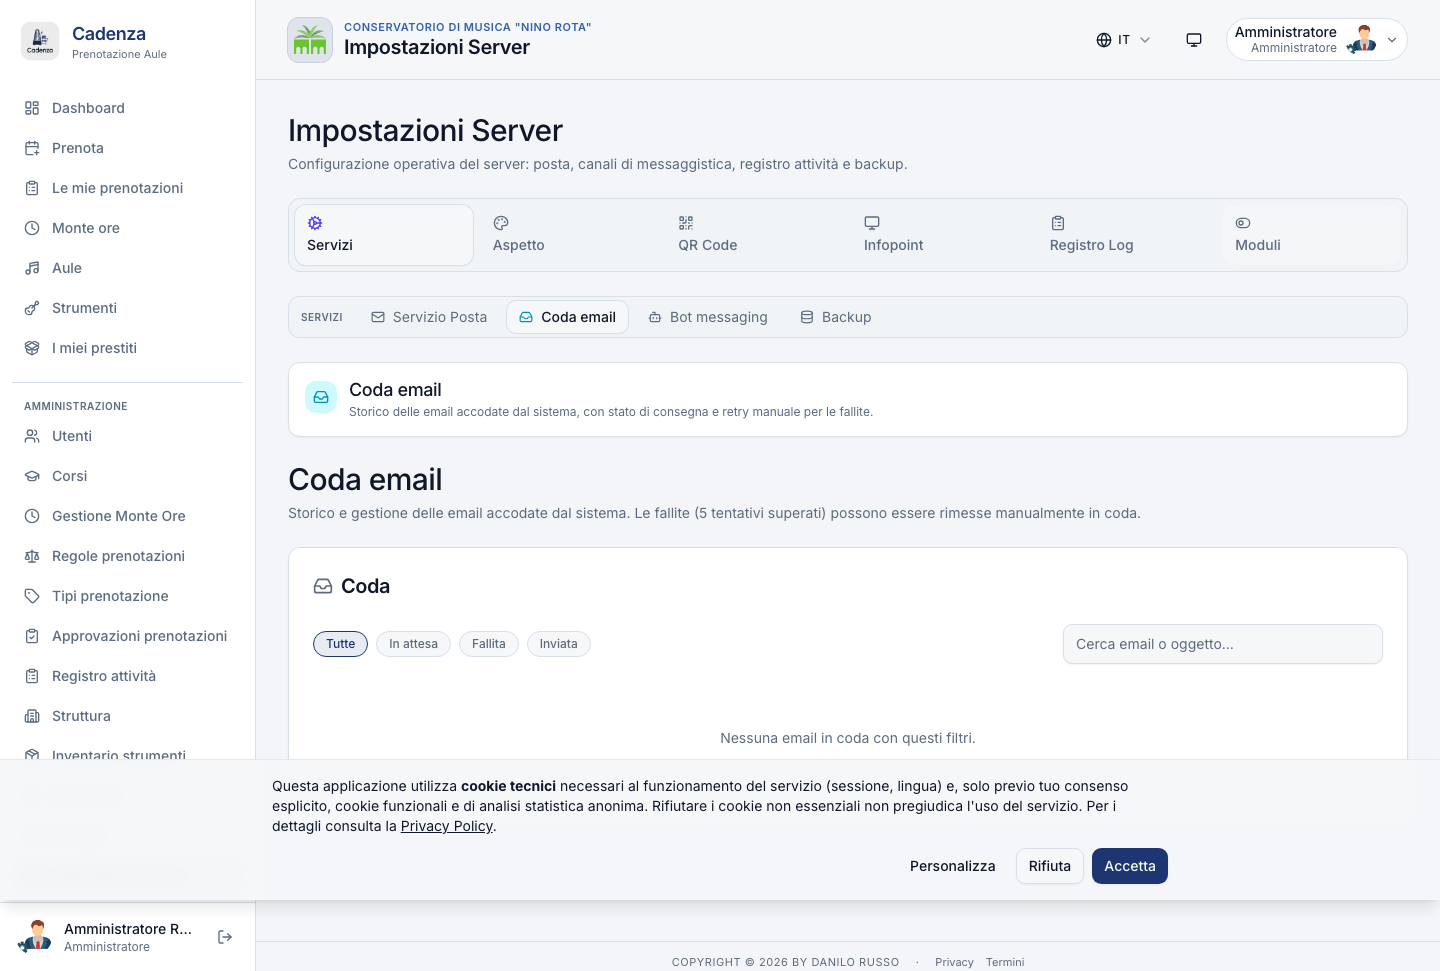
\includegraphics[width=0.95\linewidth]{screenshots/mail-outbox-overview.png}\caption*{Sotto-tab Servizi → Mail Outbox — coda email, banner salute SMTP, retry e cleanup}\end{figure}

\subsubsection{Banner di salute SMTP}


In alto, banner con 4 colori:

\begin{itemize}
  \item \textcolor{green!60!black}{$\bullet$} \textbf{Verde} --- SMTP attivo, coda pulita
  \item \textcolor{yellow!70!black}{$\bullet$} \textbf{Ambra} --- SMTP non configurato
  \item \textcolor{red}{$\bullet$} \textbf{Rossa} --- SMTP non raggiungibile + dettaglio errore
  \item \textcolor{red}{$\bullet$} \textbf{Rossa} --- Email fallite oltre il numero massimo di tentativi
\end{itemize}

Aggiornato ogni 30 secondi automaticamente.

\subsubsection{Filtri e tabella}


\begin{itemize}
  \item \textbf{Pillole stato}: Tutti · In attesa · Inviate · Fallite (dead)
  \item \textbf{Ricerca}: cerca su email destinatario / oggetto
  \item \textbf{Paginazione} prev/next
\end{itemize}

Le colonne sono: stato, tipo template, destinatario, oggetto, tentativi (\texttt{N / max}), quando (data inviata o prossimo tentativo), azioni: \textit{(ricarica)} \textbf{Riprova} (solo se "fallite") e \textit{canc.} \textbf{Elimina}.

\subsection{12.3 Servizi $\rightarrow$ Messaging}


\begin{figure}[H]\centering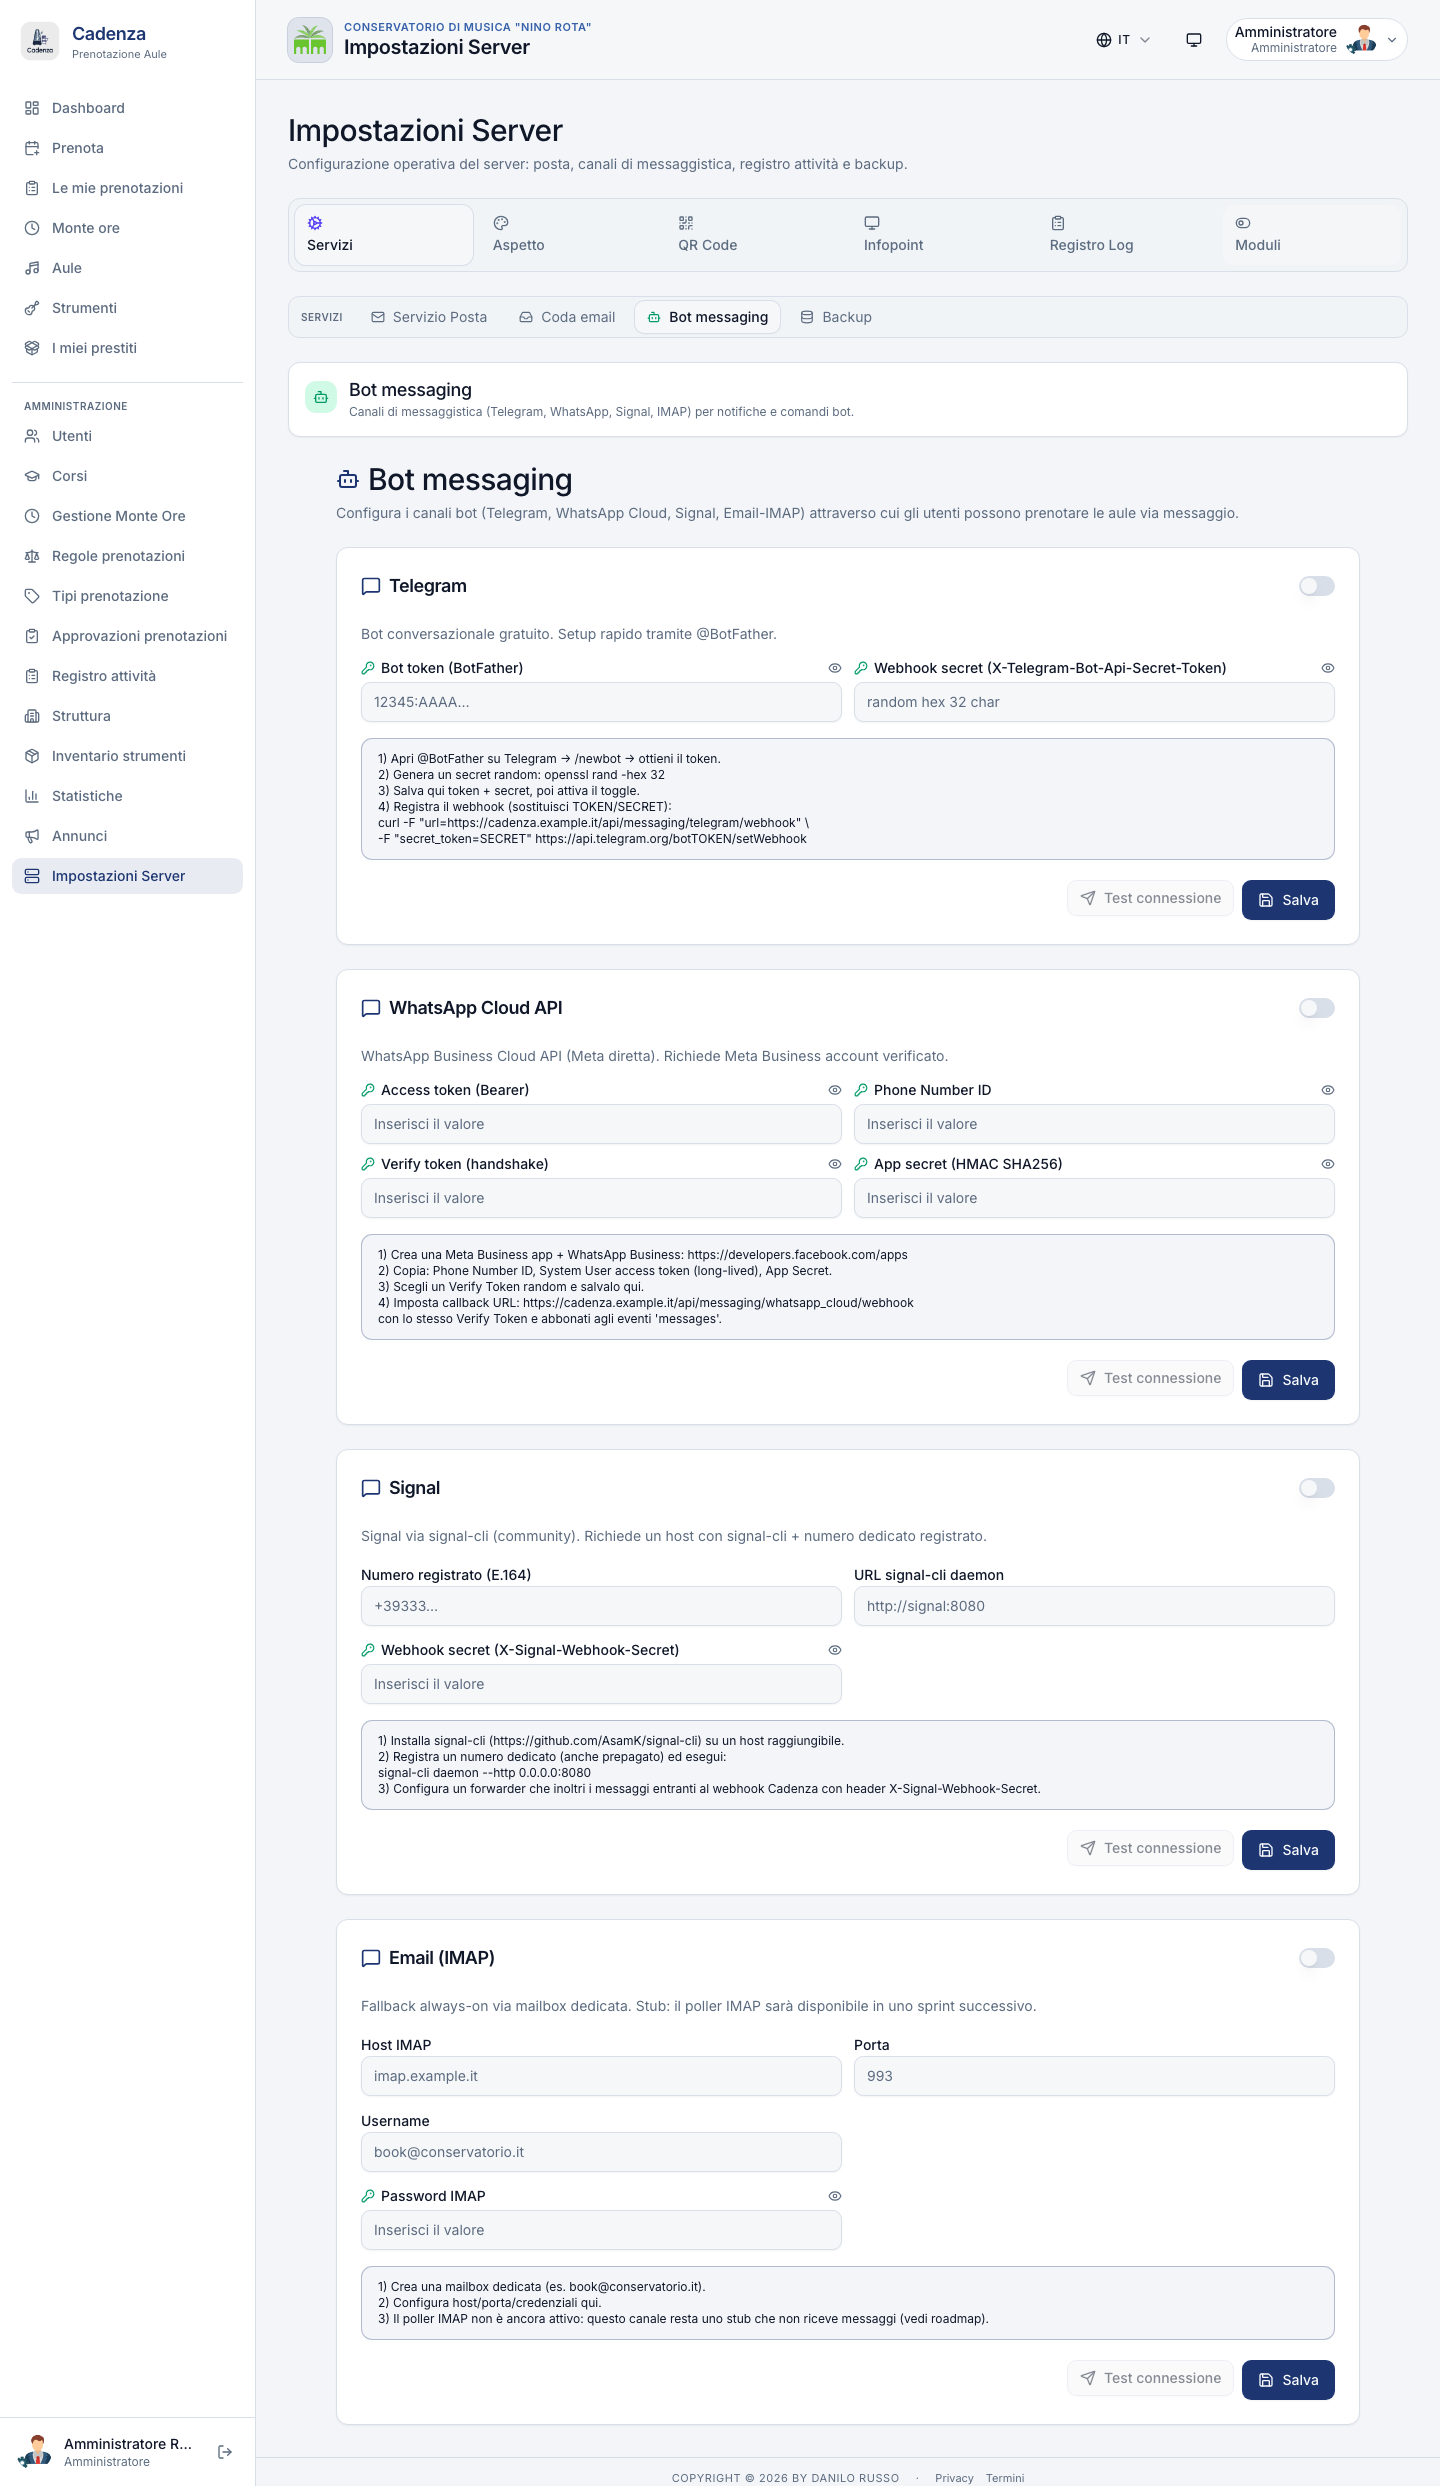
\includegraphics[width=0.95\linewidth]{screenshots/server-settings-servizi-messaging.png}\caption*{Sotto-tab Servizi → Messaging — adapter Telegram/WhatsApp/Signal/Email IMAP}\end{figure}

Una card per ogni canale (\textbf{Telegram · WhatsApp · Signal · Email/IMAP}). Ognuna ha:

\begin{itemize}
  \item Toggle abilita/disabilita
  \item Le impostazioni non-secret (host, ID, ecc.)
  \item Le credenziali secret (mostrate come \texttt{••••••} se già salvate)
  \item Una guida di setup contestuale (alert info)
  \item Eventuale risultato dell'ultimo test (alert info/error)
  \item Bottoni \textbf{Test} + \textbf{Salva}
\end{itemize}

I parametri tecnici per ciascun canale (token, secret, webhook URL) sono spiegati passo-passo in \texttt{docs/BOT-MESSAGING.md}.

\subsection{12.4 Servizi $\rightarrow$ Backups}


\begin{figure}[H]\centering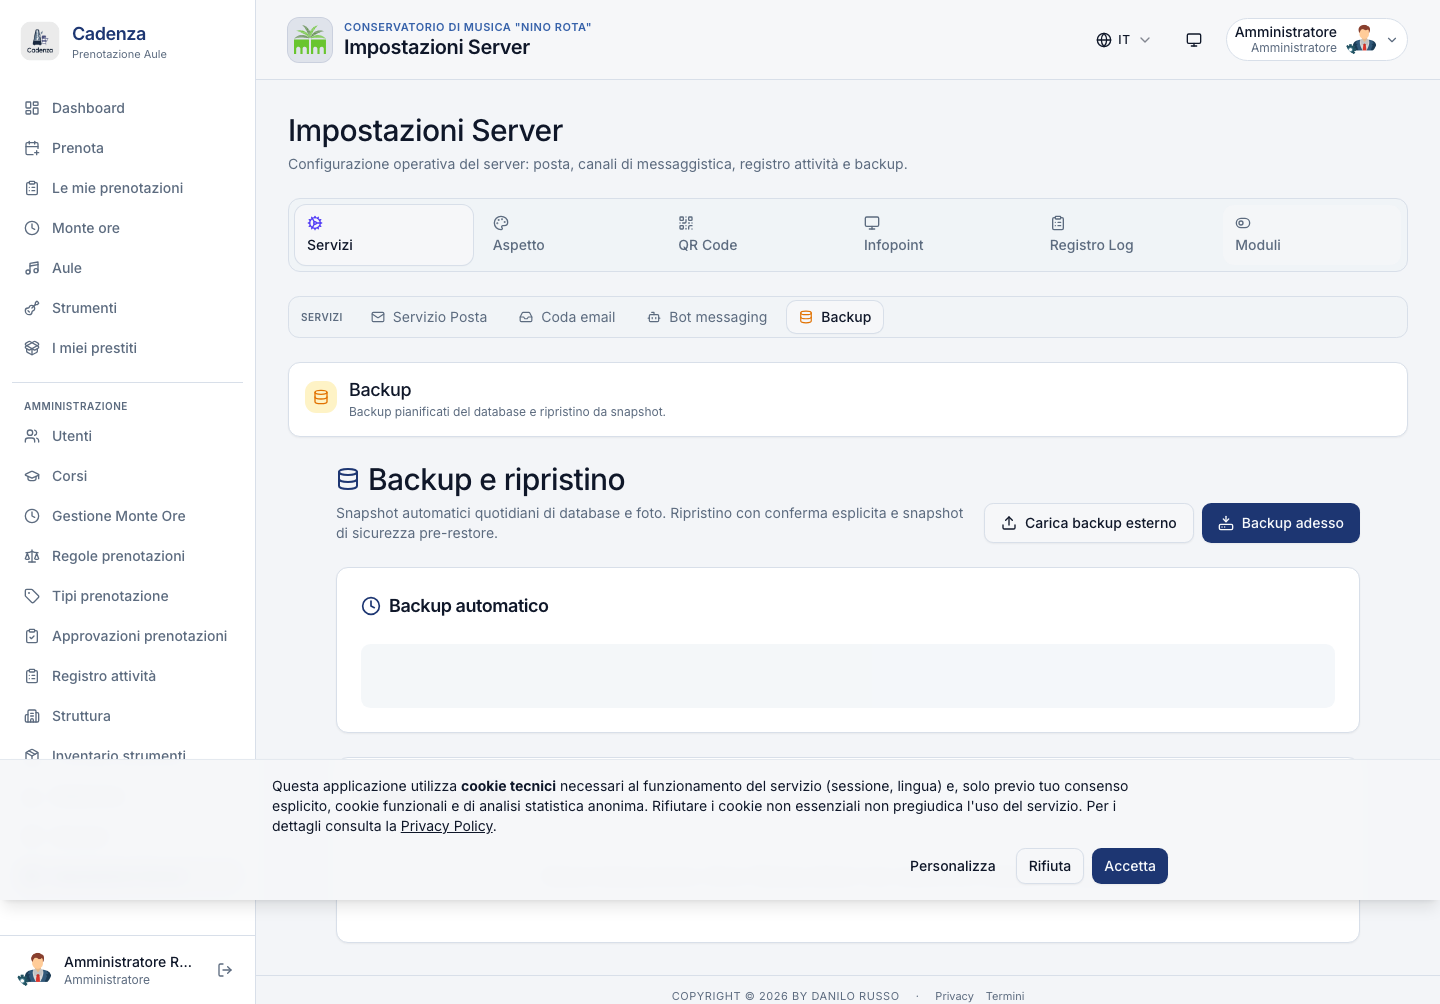
\includegraphics[width=0.95\linewidth]{screenshots/server-settings-backups.png}\caption*{Sotto-tab Servizi → Backups — scheduler, lista backup con restore e upload remoto}\end{figure}

\subsubsection{Card "Scheduler"}


Mostra: stato (Attivo/Disattivato), orario pianificato, prossimo run e --- sotto --- l'esito dell'\textbf{ultimo run} (\textcolor{green!60!black}{\checkmark{}} verde o \textcolor{red}{$\times$} rosso con dettaglio).

Configurazione (in modalità modifica):

\begin{table}[H]
\centering
\small
\begin{tabularx}{\linewidth}{|X|X|}
\hline
\rowcolor{tableheader} Campo & Descrizione \\
\hline
Auto enabled & Accendi/spegni il backup automatico \\
\hline
Ora · Minuto pianificati & A che ora locale parte \\
\hline
Quanti giornalieri tenere & 1--365 \\
\hline
Quanti settimanali tenere & 1--104 \\
\hline
Quanti mensili tenere & 1--60 \\
\hline
Auto restart & Riavvia il backend dopo un restore \\
\hline
\end{tabularx}
\end{table}


\subsubsection{Card "Lista backup"}


Tabella con file, data, size, e azioni:

\begin{itemize}
  \item  \textbf{Download} --- scarica il \texttt{.tar.gz}
  \item \textit{(ricarica)} \textbf{Restore} (con conferma) --- ripristina lo stato dell'istante in cui il backup è stato creato. Cadenza salva uno \textbf{snapshot pre-restore} prima di sovrascrivere, così puoi tornare indietro se ti accorgi di aver scelto il backup sbagliato. Il bottone "Riavvia backend" appare nella card di successo.
  \item \textit{canc.} \textbf{Delete} (con conferma)
\end{itemize}

In header: bottoni \textbf{+ Backup adesso} e \textbf{$\uparrow$ Upload} (per caricare un backup esterno).

\begin{quote}
Per la procedura completa di backup, restore e off-site upload (S3, Hetzner Storage Box, rclone, GPG) vedi \texttt{docs/BACKUP.md}.
\end{quote}

\subsection{12.4bis Servizi $\rightarrow$ Export Excel (business continuity)}


Sotto-tab dentro \textbf{Servizi} che permette di \textbf{continuare a operare anche se Cadenza è giù}: il backend scrive periodicamente un file \texttt{.xlsx} su disco, e una sync separata via \texttt{rclone} lo carica su un cloud personale (OneDrive, Dropbox, pCloud, iCloud, Google Drive). Se il server crasha, la portineria apre l'ultima copia del foglio dall'app cloud del telefono e sa subito chi ha l'aula 12 alle 14:30.

\subsubsection{Cosa contiene il file}


\begin{itemize}
  \item \textbf{Tab "Prenotazioni"} --- lista flat di tutte le prenotazioni confermate dei prossimi N giorni (default 30): ID, Aula, Edificio, Utente, Ruolo, Inizio, Fine, Tipo, Stato.
  \item \textbf{Tab "Griglia · \texttt{\textless{}nome sede\textgreater{}}"} --- \textbf{una tab per ogni edificio}, replica fedele del Display kiosk: matrice aule × slot 30 minuti dalle 08:00 alle 21:00 del giorno corrente. Aule ordinate per piano e poi per nome (numeric-aware: "Aula 9" prima di "Aula 10"). Celle \textbf{colorate per tipo} (\texttt{studio\_individuale} verde · \texttt{lezione} azzurro · \texttt{prova} ambra · \texttt{concerto} rosa · \texttt{altro} viola) e i blocchi che coprono più slot consecutivi appaiono come \textbf{una sola cella fusa} (proprio come i rettangoli del Display).
  \item \textbf{Tab "Info sync"} --- quando è stato fatto l'ultimo export, durata, conteggio righe, finestra coperta.
\end{itemize}

\subsubsection{Pannello admin}


Apri \textbf{Impostazioni server $\rightarrow$ Servizi $\rightarrow$ Export Excel}. Vedi:

\begin{itemize}
  \item Badge stato (Disattivato · In attesa primo export · Attivo · Errore)
  \item Tre metriche: ultimo export (con durata), record sincronizzati, dimensione file
  \item Path del file su disco (esempio: \texttt{/var/cadenza/sync/cadenza-prenotazioni.xlsx})
  \item Bottone \textbf{"Rigenera ora"} --- forza un export immediato fuori dal tick automatico
  \item Bottone \textbf{"Scarica ora"} --- scarica il file \texttt{.xlsx} direttamente nel browser, senza passare dal cloud (utile per verifica)
\end{itemize}

\subsubsection{Attivazione (server-side, una volta sola)}


Il modulo è \textbf{disattivato di default}. Per attivarlo serve toccare il file \texttt{backend/.env} sul VPS (le impostazioni qui sono ops-level, non DB):

\begin{lstlisting}
EXCEL_EXPORT_ENABLED=true
EXCEL_EXPORT_PATH=/var/cadenza/sync/cadenza-prenotazioni.xlsx
EXCEL_EXPORT_TICK_MIN=10            # ogni quanti minuti generare il file (1–60)
EXCEL_EXPORT_LOOKAHEAD_DAYS=30      # finestra di prenotazioni da esportare
\end{lstlisting}

Dopo il restart del backend il modulo è attivo e il primo export parte entro \texttt{EXCEL\_EXPORT\_TICK\_MIN} minuti.

\subsubsection{Sync verso il cloud (rclone)}


Il backend scrive solo su disco locale. Per averlo sul telefono della portineria serve un sync separato gestito dal sistema operativo:

\begin{enumerate}
  \item Installa \texttt{rclone} sul VPS (\texttt{curl https://rclone.org/install.sh | sudo bash}).
  \item Configura un remote come utente \texttt{cadenza}: \texttt{sudo -u cadenza rclone config} --- scegli OneDrive/Dropbox/pCloud (account personali bastano, non serve abbonamento aziendale).
  \item Esegui \texttt{sudo bash scripts/setup-rclone-sync.sh cadenza-cloud CadenzaBackup} --- lo script crea la cartella \texttt{/var/cadenza/sync/} con i permessi giusti, verifica che il remote sia raggiungibile e installa un cron che sincronizza ogni 10 minuti.
  \item La portineria apre l'app OneDrive/Dropbox sul telefono e vede il file aggiornato.
\end{enumerate}

\begin{quote}
Procedura completa passo-passo (con headless authorization per server senza browser, troubleshooting, frequenza vs freschezza): \href{EXCEL_SYNC.md}{docs/EXCEL\_SYNC.md}.
\end{quote}

\subsubsection{Direzione \textbf{volutamente} unidirezionale}


Le modifiche fatte al foglio dal telefono \textbf{NON tornano in Cadenza} al ripristino. Questa è una scelta deliberata per evitare conflict resolution complessa (chi vince? il foglio o il DB?). Procedura raccomandata durante un downtime esteso:

\begin{enumerate}
  \item Crea un foglio separato chiamato "\textbf{Prenotazioni manuali (offline)}" e annota lì le nuove prenotazioni urgenti.
  \item Quando Cadenza torna online, trascrivi a mano le righe annotate dentro l'app.
  \item Niente automatismi, niente sorprese.
\end{enumerate}

\subsection{12.5 Aspetto}


\begin{figure}[H]\centering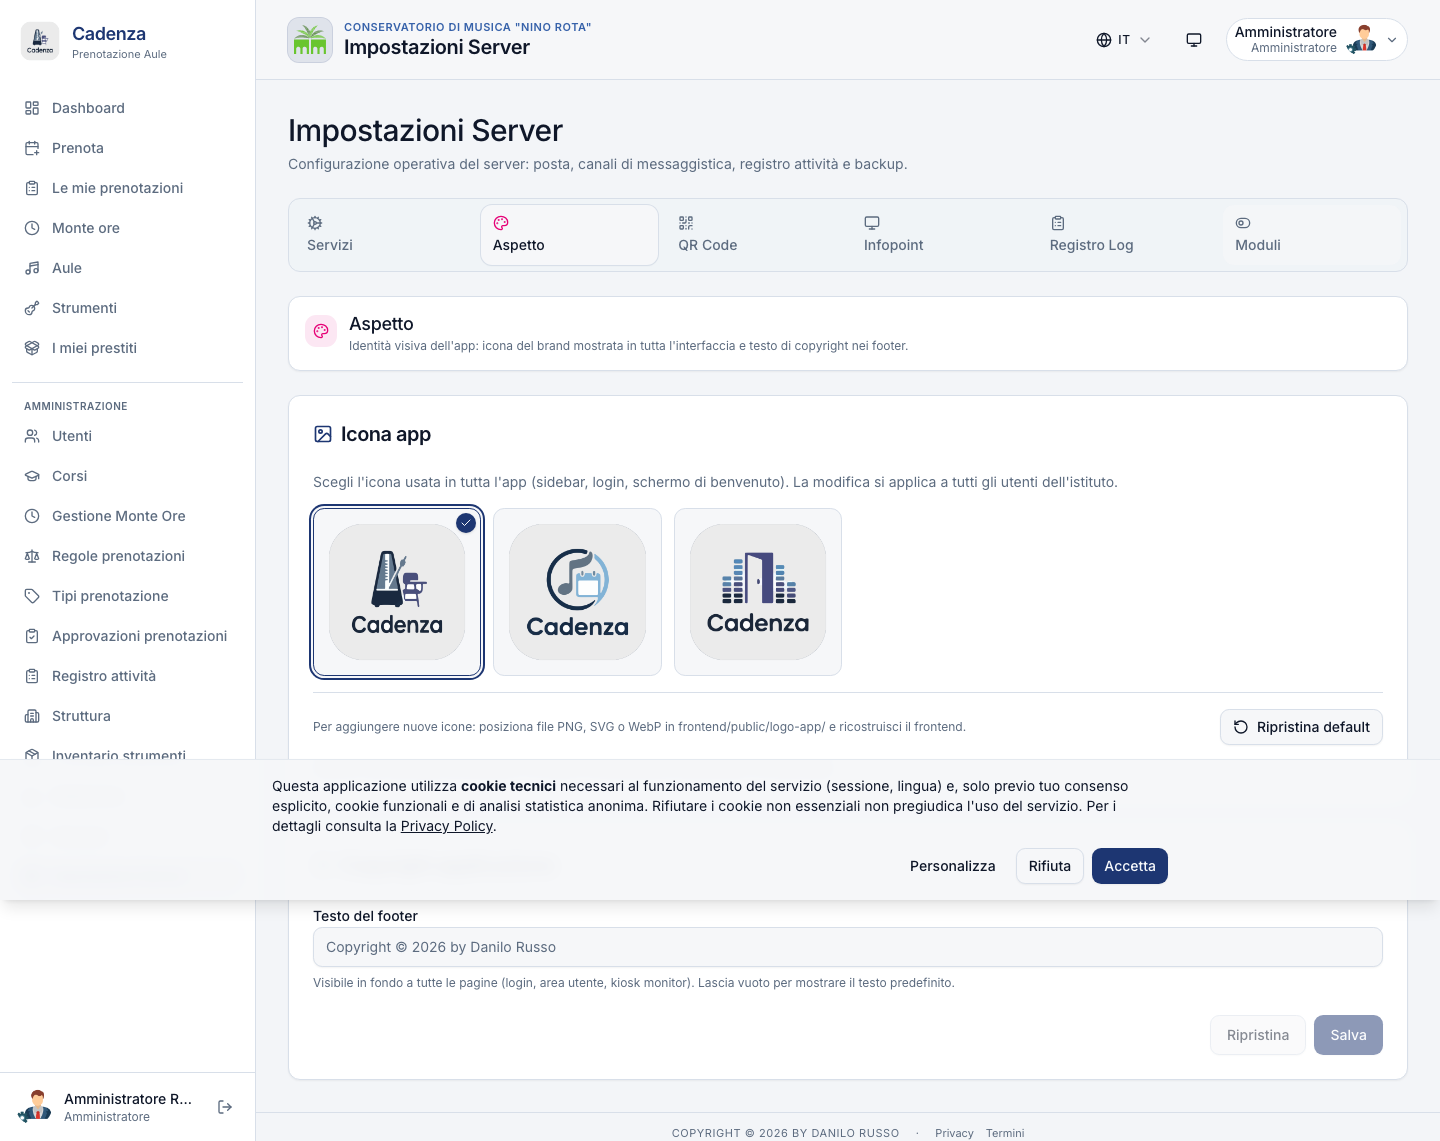
\includegraphics[width=0.95\linewidth]{screenshots/server-settings-aspetto.png}\caption*{Sotto-tab Aspetto — logo, icona app, copyright}\end{figure}

Due card:

\begin{itemize}
  \item \textbf{Icona dell'app} --- upload del logo brand (PNG/SVG). Il logo appare nella sidebar, sul login, sul display kiosk.
  \item \textbf{Copyright} --- testi che compaiono nel footer di tutte le pagine pubbliche e sul display kiosk.
\end{itemize}

\subsection{12.6 QR Codes}


\begin{figure}[H]\centering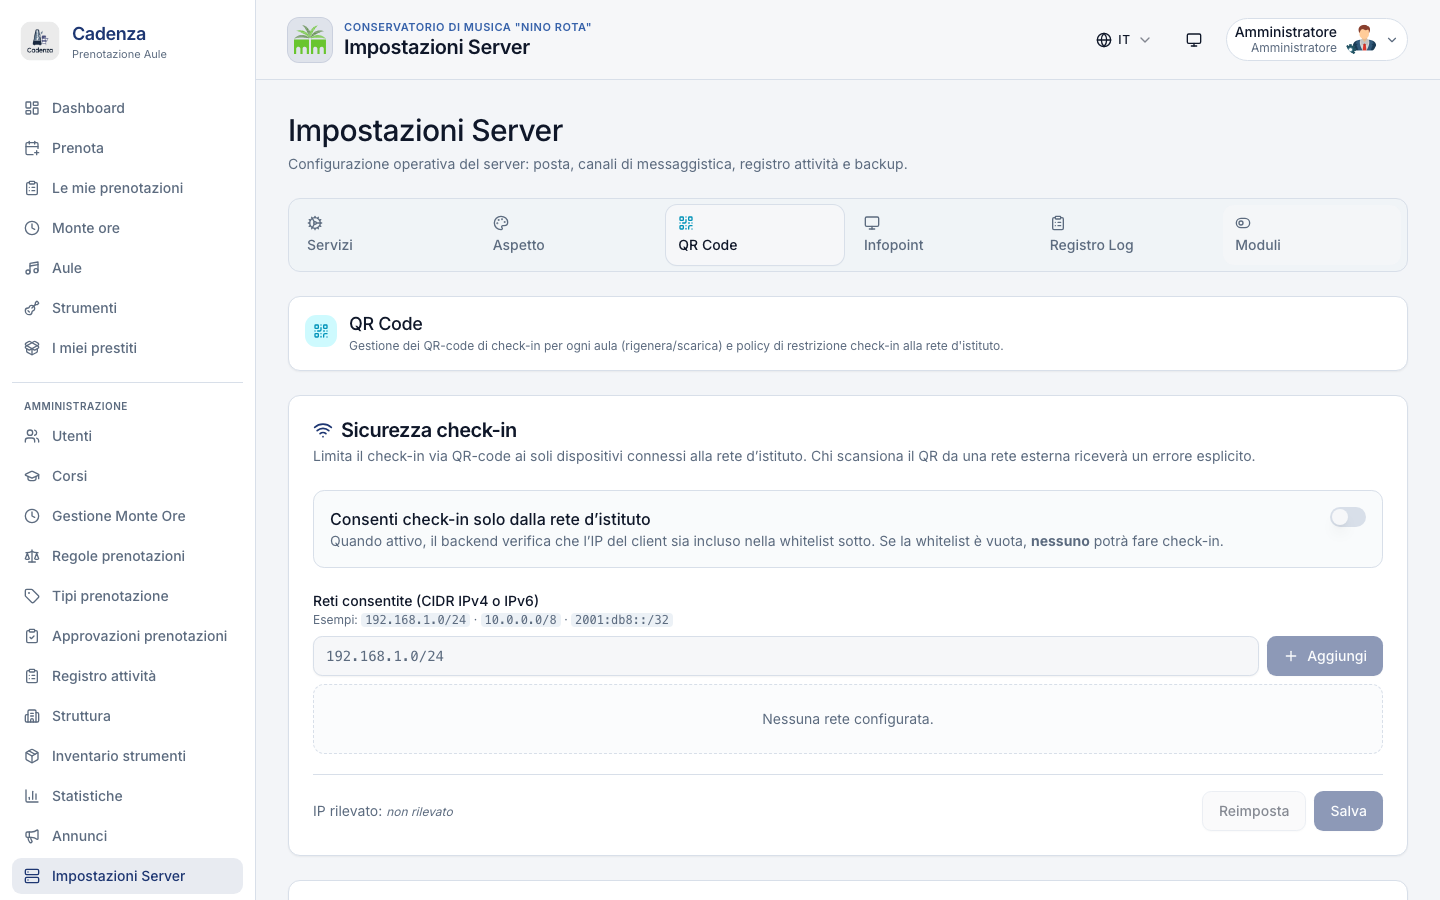
\includegraphics[width=0.95\linewidth]{screenshots/server-settings-qrcodes.png}\caption*{Sotto-tab QR Codes — sicurezza check-in IP, generazione QR per aula}\end{figure}

\subsubsection{Card "Sicurezza check-in"}


Permette di restringere il check-in (la "presentazione" all'aula tramite QR) \textbf{solo agli IP della rete interna del Conservatorio}. Configura:

\begin{itemize}
  \item \textbf{Restringi alla rete interna} (interruttore on/off)
  \item \textbf{Lista CIDR}: gli intervalli IP autorizzati (es. \texttt{192.168.1.0/24}, \texttt{10.0.0.0/8})
  \item Bottone \textbf{"Aggiungi mio IP corrente"} (utile dal browser per capire quale è il tuo IP pubblico)
\end{itemize}

Banner di aiuto:

\begin{itemize}
  \item \textbf{Loopback warning}: avvisa se l'IP rilevato è \texttt{::1} o \texttt{127.x.x.x} (sei in localhost, non in rete vera)
  \item \textbf{Rete vuota + restringi attivo}: configurazione pericolosa, \textbf{nessuno} potrebbe fare check-in. Allerta rossa.
\end{itemize}

\subsubsection{Card "QR-code per aula"}


Lista delle aule con anteprima del QR e i bottoni:

\begin{itemize}
  \item  \textbf{Scarica QR} --- il PDF A4 da affiggere in aula
  \item \textit{(ricarica)} \textbf{Rigenera} --- genera un nuovo QR (i fogli stampati vecchi diventano inutili)
\end{itemize}

In header: \textbf{Rigenera tutti} --- operazione di emergenza (es. dopo un incidente di sicurezza).

\subsection{12.7 Display Kiosk (admin)}


\begin{figure}[H]\centering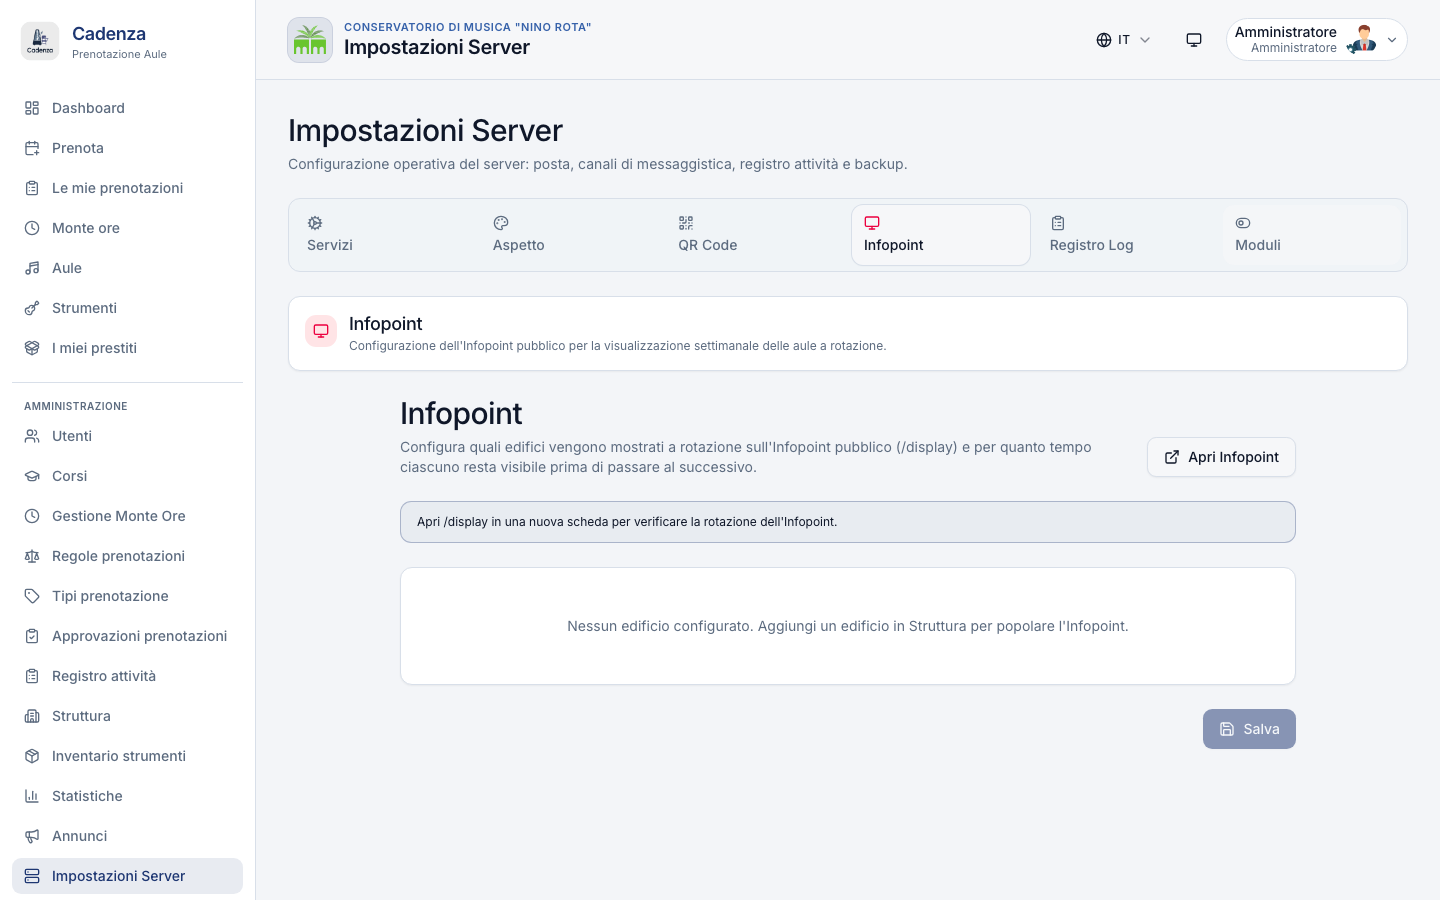
\includegraphics[width=0.95\linewidth]{screenshots/server-settings-display.png}\caption*{Sotto-tab Display kiosk — rotazione edifici, concerti, annunci, privacy}\end{figure}

Pagina di configurazione globale dello schermo \texttt{/display} esposto al pubblico nelle aule.

\subsubsection{Card "Rotazione prenotazioni"}


Master toggle on/off + tabella edifici. Per ogni edificio: dot color + nome, conteggio aule, switch abilita/disabilita, l'\textbf{intervallo di rotazione} (5--600 secondi) e la \textbf{modalità di vista} della tabella prenotazioni:

\begin{table}[H]
\centering
\small
\begin{tabularx}{\linewidth}{|X|X|}
\hline
\rowcolor{tableheader} Modalità & Descrizione \\
\hline
\textbf{Settimana} (default) & Matrice aule × giorni Lun-Sab. Utile per la pianificazione settimanale. \\
\hline
\textbf{Giorno corrente} & Matrice aule (righe) × slot 30 min 08:00--21:00 (colonne) del giorno corrente, con celle colorate per tipo prenotazione e blocchi multi-slot fusi. Replica fedele della "Griglia oggi" del foglio Excel. Più informativa per la portineria che vuole sapere a colpo d'occhio chi ha quale aula adesso. \\
\hline
\end{tabularx}
\end{table}


La modalità è \textbf{per-edificio}: la sede principale può mostrare la settimana e una sede più piccola solo l'oggi. Disattivando il master della rotazione, l'intera tabella diventa opaca.

\subsubsection{Card "Link diretti per sede"}


Tabelloni di ingresso che mostrano \textbf{solo una sede} invece della rotazione completa. L'admin trova in questa card l'URL pronto da copiare per ogni edificio.

Sintassi accettate dal parser URL (priorità decrescente):

\begin{table}[H]
\centering
\small
\begin{tabularx}{\linewidth}{|X|X|}
\hline
\rowcolor{tableheader} URL & Comportamento \\
\hline
\texttt{/display} & Rotazione completa di tutti gli edifici abilitati (default). \\
\hline
\texttt{/display?b=\textless{}codice\textgreater{}} & Match esatto sul \texttt{code} dell'edificio (es. \texttt{/display?b=CENT}). Più stabile perché il code non cambia se l'admin rinomina la sede. \\
\hline
\texttt{/display?building=\textless{}slug\textgreater{}} & Alias verboso, identico a \texttt{?b=}. \\
\hline
\texttt{/display?\textless{}slug\textgreater{}} & Scorciatoia "key-boolean": una sola chiave senza valore (es. \texttt{/display?centrale}, \texttt{/display?radar}). Matcha contro \texttt{code} esatto, poi \texttt{name} esatto, poi \texttt{name} come substring (es. \texttt{centrale} matcha "Sede Centrale"). \\
\hline
\end{tabularx}
\end{table}


La card mostra una riga per ogni edificio con:
\begin{itemize}
  \item \textbf{Apri} --- apre il kiosk in una nuova scheda (utile per testare prima di passare l'URL al monitor)
  \item \textbf{Copia} --- copia l'URL completo negli appunti (con feedback "Copiato!" 2s)
\end{itemize}

Se lo slug non matcha alcun edificio (es. typo nell'URL), Cadenza ricade automaticamente sulla rotazione completa per non lasciare lo schermo vuoto.

\begin{quote}
\textbf{Suggerimento operativo}: assegna un \texttt{code} breve a ogni edificio in Struttura (es. \texttt{CENT}, \texttt{RADAR}, \texttt{STORICO}). I link basati su code sono più robusti dei link basati su name, perché il nome può cambiare nel tempo. Gli URL \texttt{/display?\textless{}slug\textgreater{}} funzionano comunque grazie al fallback substring.
\end{quote}

\subsubsection{Card "Concerti"}


\begin{table}[H]
\centering
\small
\begin{tabularx}{\linewidth}{|X|X|}
\hline
\rowcolor{tableheader} Campo & Descrizione \\
\hline
Giorni look-ahead & Da 0 a 365 \\
\hline
Numero massimo & Da 0 a 50 (\texttt{0} = tutti) \\
\hline
Intervallo (sec) & Da 5 a 600 \\
\hline
\end{tabularx}
\end{table}


\subsubsection{Card "Annunci"}


\begin{table}[H]
\centering
\small
\begin{tabularx}{\linewidth}{|X|X|}
\hline
\rowcolor{tableheader} Campo & Descrizione \\
\hline
Numero massimo & Da 0 a 30 (\texttt{0} = tutti) \\
\hline
Intervallo (sec) & Da 5 a 600 \\
\hline
Solo pinnati & Mostra solo gli annunci con badge "Pin" \\
\hline
\end{tabularx}
\end{table}


In fondo: bottone \textbf{Salva} (disabilitato se non hai modificato nulla).

\begin{quote}
\textbf{Anteprima}: il pulsante in header apre \texttt{/display} in nuova scheda --- utile per verificare la rotazione in tempo reale dopo aver salvato.
\end{quote}

\subsection{12.8 Audit Log}


\begin{figure}[H]\centering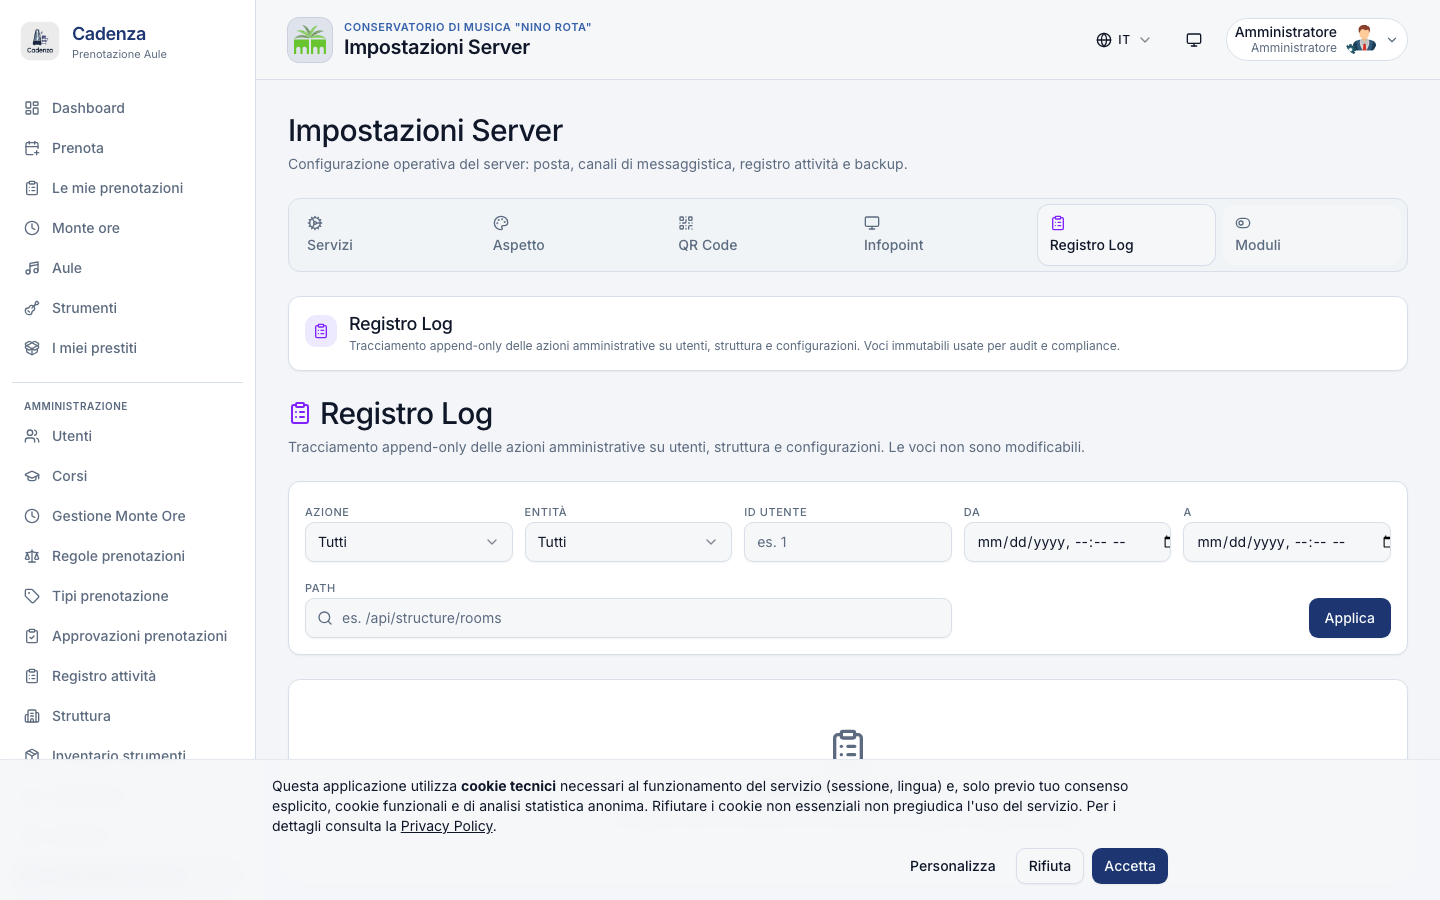
\includegraphics[width=0.95\linewidth]{screenshots/server-settings-audit-log.png}\caption*{Sotto-tab Audit Log — tabella eventi con filtri action/target/actor/date}\end{figure}

URL: \texttt{/admin/audit-log} (sub-tab di Server Settings; rinominato in "Registro Log" per distinguerlo dal "Registro attività" operativo di §7.2).

\subsubsection{Filtri}


\begin{itemize}
  \item \textbf{Action}: tutti · POST · PUT · PATCH · DELETE
  \item \textbf{Target Type}: tipo oggetto interessato (utente, prenotazione, regola, ecc.)
  \item \textbf{Actor ID}: ID dell'admin
  \item \textbf{Date From / To}: range temporale
  \item \textbf{Path Search}: testo libero sulla path API
\end{itemize}

Bottoni \textbf{Apply} / \textbf{Reset} (Reset visibile solo se ci sono filtri attivi).

\subsubsection{Tabella}


50 righe per pagina. Colonne: quando, attore (nome + email), action (badge mono colorato), target, path, status code (verde se OK, rosso se $\geq$400).

\textbf{Click sulla riga} $\rightarrow$ si espande mostrando il payload, la risposta, l'IP e lo User-Agent.

\subsubsection{Conservazione e prune}


Per conformità GDPR i record dell'audit log oltre i \textbf{730 giorni} vengono rimossi automaticamente dal sistema. Prima del prune, Cadenza esegue un \textbf{export firmato} in \texttt{backups/audit/} (file \texttt{.gz} + sidecar \texttt{.hmac} con la chiave HMAC), così gli archivi storici restano disponibili per audit forensic. Solo se l'export riesce, il prune procede; in caso contrario i dati vengono preservati per il prossimo tentativo.

\subsection{12.9 Moduli}


\begin{figure}[H]\centering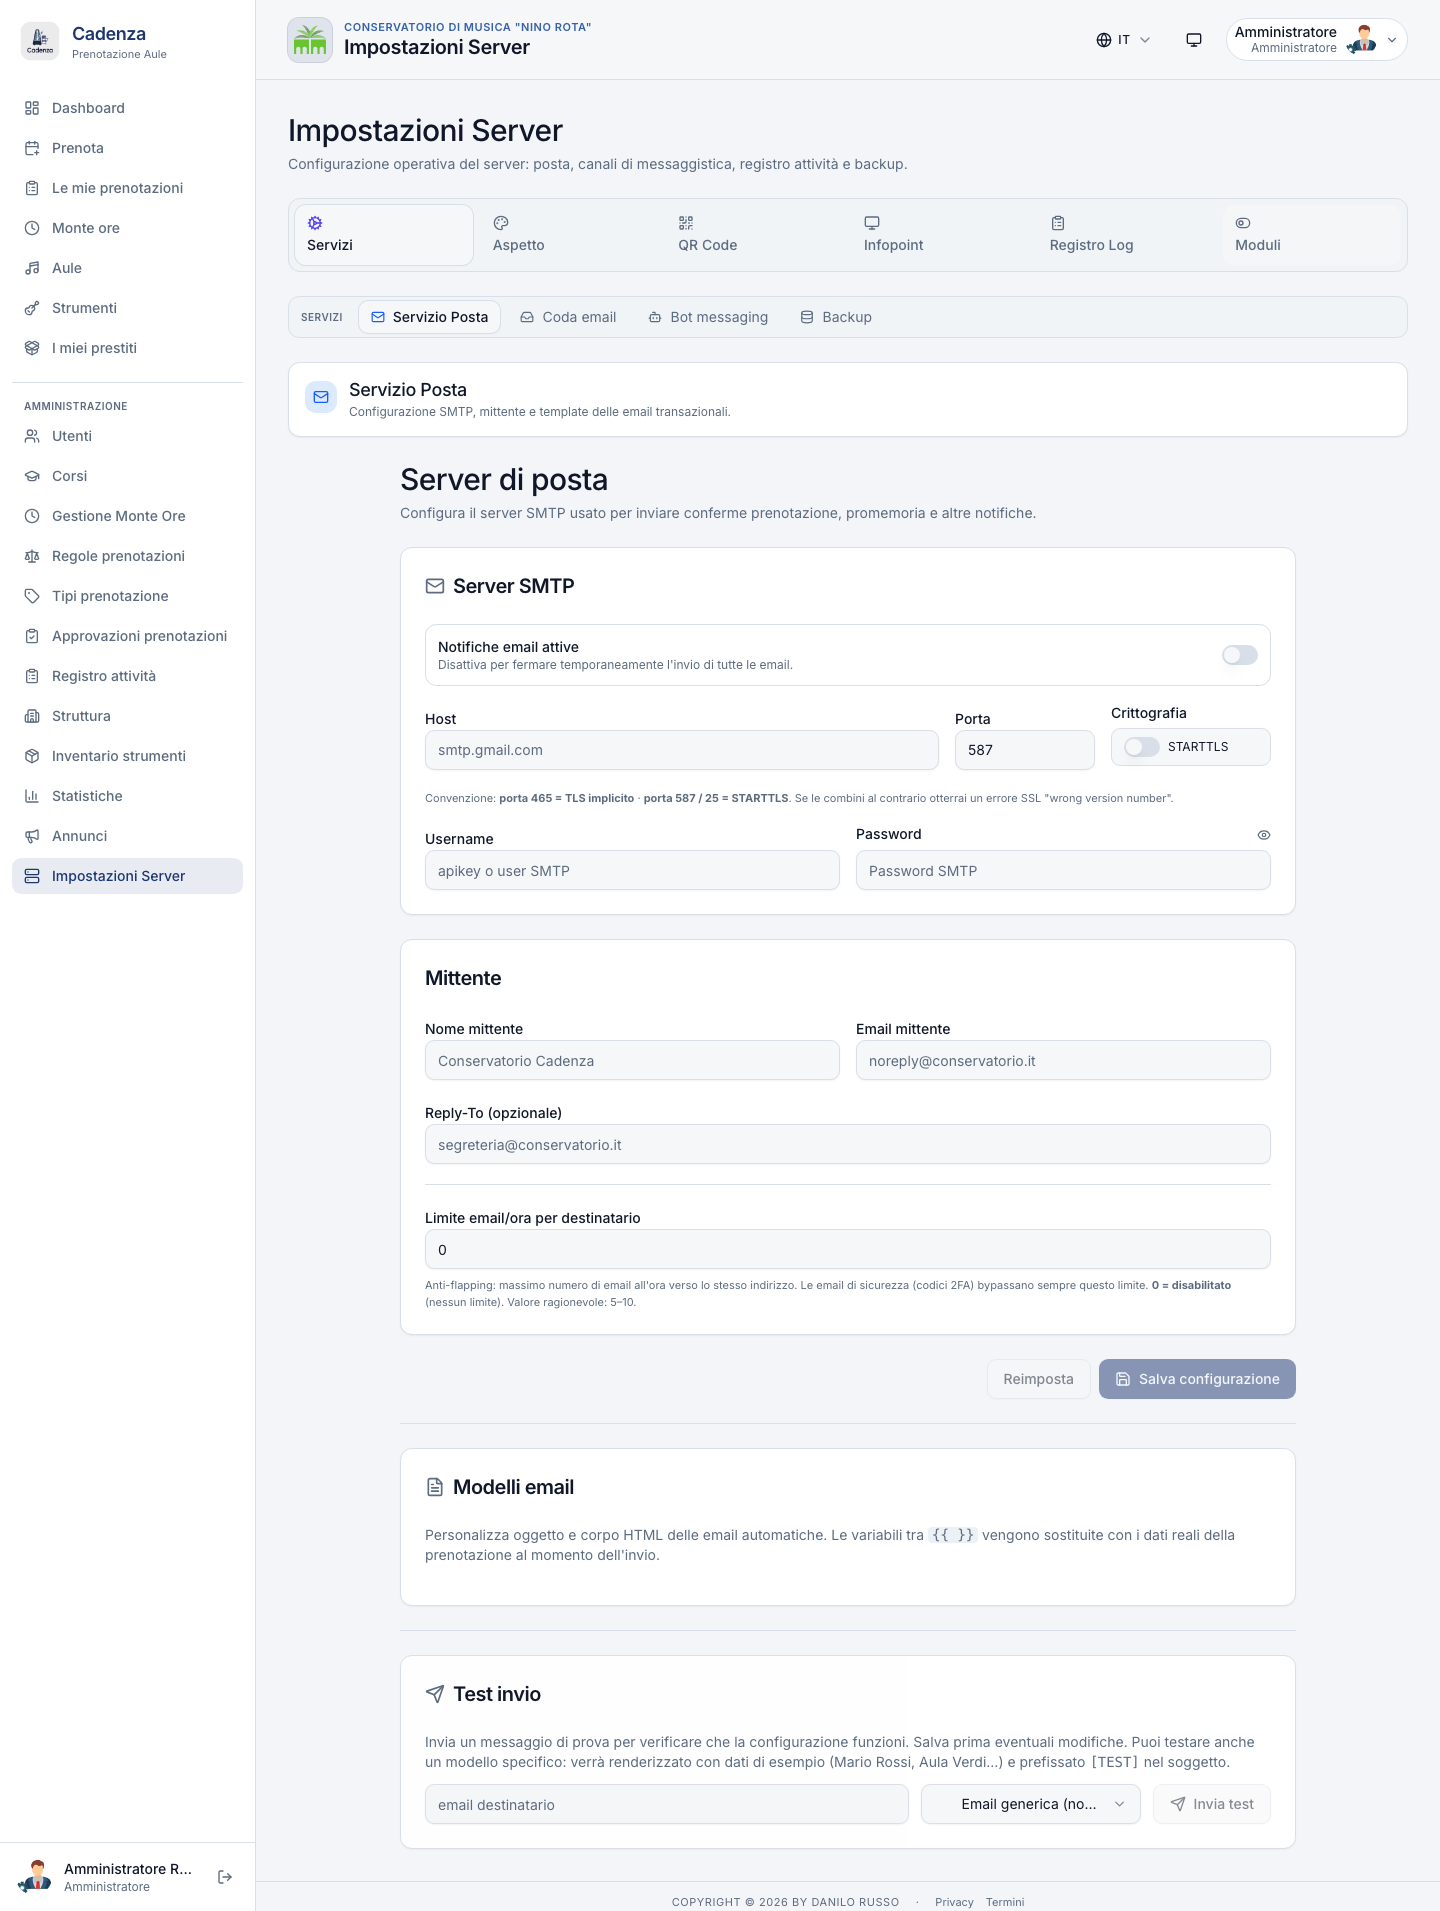
\includegraphics[width=0.95\linewidth]{screenshots/server-settings-moduli.png}\caption*{Sotto-tab Moduli — toggle Monte Ore e Prestito strumenti per nascondere voci sidebar}\end{figure}

Card con due interruttori:

\begin{table}[H]
\centering
\small
\begin{tabularx}{\linewidth}{|X|X|}
\hline
\rowcolor{tableheader} Modulo & Effetto \\
\hline
\textbf{Monte Ore docenti} & Nasconde le voci \texttt{/monte-ore} (utente) e \texttt{/admin/monte-ore} (sidebar) \\
\hline
\textbf{Prestito strumenti} & Nasconde \texttt{/instruments}, \texttt{/my-loans}, \texttt{/admin/instruments} \\
\hline
\end{tabularx}
\end{table}


\begin{quote}
\textbf{Importante}: i toggle sono \textbf{puramente di presentazione}. Il backend resta sempre attivo:  - I dati esistenti \textbf{non vengono cancellati} - Le rotte API continuano a funzionare (deep-link, integrazioni esterne, bookmark) - Riattivando il modulo i link tornano subito visibili
\end{quote}

\medskip\hrule\medskip

\section{13. Integrazioni Isidata}


URL: \texttt{/admin/integrations/isidata} --- oppure dialog modale dalla pagina Utenti (§3.6).

\subsection{13.1 Layout a 3 step}


\subsubsection{Step 1: Upload}


Trascini il file \texttt{.xlsx}, \texttt{.xls} o \texttt{.csv} nella drop area (oppure clicchi per scegliere). Sotto, una textarea collassabile permette di forzare un mapping personalizzato delle colonne quando i nomi nel file sono diversi da quelli standard (vedi §13.3).

\subsubsection{Step 2: Anteprima (preview)}


Cadenza fa il parsing del file e mostra \textbf{4 KPI tile} in alto:

\begin{itemize}
  \item \textbf{Da creare} (verde) --- nuovi utenti che entreranno in Cadenza
  \item \textbf{Da aggiornare} (blu) --- utenti già presenti i cui dati cambieranno
  \item \textbf{Da disattivare} (ambra) --- utenti che erano stati linkati a Isidata ma non sono più nel nuovo export
  \item \textbf{Letti totali} --- quante righe sono state effettivamente lette dal file
\end{itemize}

Sotto le KPI, 3 sezioni filtrabili con i dettagli di ogni cambio + eventuali warning. \textbf{Nessuna modifica viene scritta} in questa fase.

\subsubsection{Step 3: Done}


Card "Importazione completata" con i numeri finali e il bottone "Importa un altro".

\subsection{13.2 Flusso a 2 step (preview $\rightarrow$ apply)}


L'import è in \textbf{due fasi distinte}, per dare a chi lo lancia il tempo di rivedere ciò che cambierà prima di confermare:

\begin{enumerate}
  \item \textbf{Preview}: il file viene caricato e analizzato. Cadenza memorizza temporaneamente il file (per max 10 minuti) e ne calcola un'impronta digitale.
  \item \textbf{Apply}: confermi l'import. Cadenza riapre il file, ricontrolla l'impronta digitale e --- se il file è stato sostituito nel frattempo --- rifiuta l'apply per evitare confusione. Esegue create / update / disattivazione in transazione: o tutto va a buon fine, o nulla viene scritto.
\end{enumerate}

I nuovi utenti nascono in stato \textbf{\texttt{pending}} (vanno approvati esplicitamente dalla pagina Approvazioni). Gli utenti orfani non vengono mai cancellati fisicamente: solo \texttt{isActive=false} con nota "Non più presente nell'export Isidata del YYYY-MM-DD". Riapparire in un export futuro li riattiva.

\subsection{13.3 Mapping personalizzato per istituto}


Se il vostro export Isidata ha header diversi da quelli auto-riconosciuti, scrivi un piccolo JSON nella textarea "Override colonne" durante l'upload. Esempio:

\begin{lstlisting}
{
  "externalId": "Numero Matricola",
  "email": "Email Istituzionale",
  "courseCode": "Codice Indirizzo"
}
\end{lstlisting}

I target consentiti sono: \texttt{externalId}, \texttt{email}, \texttt{firstName}, \texttt{lastName}, \texttt{role}, \texttt{matricola}, \texttt{courseCode}, \texttt{courseName}, \texttt{status}, \texttt{birthDate}. Altri target vengono ignorati.

\begin{quote}
Per la procedura dettagliata (creazione export Isidata, esempi di mapping per ogni Conservatorio, audit trail) vedi \texttt{docs/INTEGRATIONS-ISIDATA.md}.
\end{quote}

\medskip\hrule\medskip

\section{14. Operazioni periodiche e best practice}


\subsection{14.1 All'inizio dell'anno accademico (settembre)}


\begin{enumerate}
  \item Aggiorna le impostazioni Monte Ore: nuove date anno + finestre.
  \item Inserisci tutte le sospensioni del calendario didattico (festività + ferie + sessioni esami).
  \item Apri la finestra inserimento proposte.
  \item Notifica i docenti via Annuncio o email diretta.
  \item Importa anagrafica studenti aggiornata (Isidata o CSV manuale).
  \item Verifica che le aule in ristrutturazione siano marcate come non prenotabili.
  \item Aggiorna le quote stagionali (es. orario serale 18--22).
\end{enumerate}

\subsection{14.2 Settimanale}


\begin{itemize}
  \item \textbf{Lunedì mattina}: controlla \textit{Approvazioni} (badge sidebar) $\rightarrow$ approva/rifiuta in batch.
  \item \textbf{Mercoledì mattina}: controlla le \textit{Variazioni Monte Ore} $\rightarrow$ approva/rifiuta.
  \item \textbf{Venerdì pomeriggio}: controlla \textit{Statistiche} $\rightarrow$ individua aule sotto-utilizzate o utenti con no-show seriali.
  \item \textbf{Giornaliero}: occhio al banner SMTP nella \textit{Mail Outbox} --- se diventa rosso, controlla le mail rimbalzate.
\end{itemize}

\subsection{14.3 Mensile}


\begin{itemize}
  \item Esporta backup off-site (oltre allo Storage Box automatico --- copia su un disco fisico in cassaforte come ulteriore garanzia).
  \item Audit log review (filtra azioni di delete e cambio ruolo del mese).
  \item Aggiornamento policy se cambia normativa (Garante / AgID).
\end{itemize}

\subsection{14.4 Annuale}


\begin{itemize}
  \item Rivedi le quote (le abitudini di prenotazione cambiano).
  \item Esporta tutti i Monte Ore approvati come PDF per archivio amministrativo.
  \item Restore test da backup (esercizio di disaster recovery --- vedi \texttt{docs/DISASTER\_RECOVERY.md}).
\end{itemize}

\medskip\hrule\medskip

\section{15. Troubleshooting}


\subsection{"L'utente dice di non poter prenotare ma la regola sembra OK"}


Il messaggio di errore che riceve l'utente indica esattamente quale regola è stata violata. Chiedi che ti faccia uno screenshot dell'errore o di leggerti il testo. I casi tipici:

\begin{itemize}
  \item "Hai superato le ore settimanali consentite" $\rightarrow$ vedi le quote in §6.2 e la regola del ruolo in §6.1
  \item "Aula non prenotabile in questa fascia oraria" $\rightarrow$ potrebbe esserci un'eccezione \texttt{block} attiva (§6.3)
  \item "Hai un'altra prenotazione in corso in un'altra aula" $\rightarrow$ un docente non può essere in due posti, è normale
\end{itemize}

\subsection{"Le prenotazioni Monte Ore non appaiono nel calendario"}


\begin{enumerate}
  \item Verifica che la proposta sia in stato \textbf{Generata} (non solo "Approvata").
  \item Apri la proposta dal \texttt{/admin/monte-ore} $\rightarrow$ sezione "Slot generati" $\rightarrow$ controlla che siano materializzati.
  \item Se la proposta è ferma su "Approvata", c'è stato un errore di sovrapposizione nella generazione: leggi il report nel campo "Note generation" per capire quale slot ha bloccato il batch.
\end{enumerate}

\subsection{"Il backup notturno non parte"}


\begin{enumerate}
  \item \texttt{Impostazioni Server → Servizi → Backups} $\rightarrow$ verifica l'ultimo run.
  \item Se errore, leggi il dettaglio (Storage Box raggiungibile? Spazio sufficiente?).
  \item Esegui un backup manuale per validare il setup.
\end{enumerate}

\subsection{"Voglio annullare massivamente le prenotazioni di un'aula in ristrutturazione"}


\begin{enumerate}
  \item Vai su \textbf{\texttt{/admin/activity-log}} (Registro attività, vedi §7.2).
  \item Cerca per nome aula + filtra per range date.
  \item Selezione multipla $\rightarrow$ \textbf{Cancella selezionate} con motivo broadcast $\rightarrow$ email automatica a tutti gli utenti coinvolti.
\end{enumerate}

\begin{quote}
Per chiusure pianificate (ristrutturazione di settimane), valuta invece di creare un'eccezione \texttt{block} da §6.3 --- Cadenza ti propone direttamente la lista delle prenotazioni da cancellare con badge "Monte Ore" per quelle collegate al piano didattico.
\end{quote}

\subsection{"Voglio scambiare aula tra 2 prenotazioni"}


\begin{enumerate}
  \item \texttt{/admin/activity-log} (Registro attività).
  \item Seleziona \textbf{esattamente 2} prenotazioni future $\rightarrow$ bottone \textbf{"Scambia"}.
  \item Lo scambio è atomico (vedi §7.2): se nel frattempo è entrata un'altra prenotazione in mezzo, l'operazione si annulla e ritenti.
\end{enumerate}

\subsection{"Errore 'intervallo minimo violato' su prenotazioni back-to-back"}


C'è un cooldown configurato sul ruolo dell'utente (§6.1). Se è troppo alto per il caso d'uso (es. masterclass docente con lezioni back-to-back), abbassalo o crea un'eccezione mirata in §6.3.

\subsection{"Errore 'conflitto logico utente' per uno studente che però era libero"}


Lo studente ha un'altra prenotazione confermata in \textbf{un'altra aula} in quella fascia oraria. È normale che Cadenza lo blocchi (un utente non può essere in due posti). Cerca tra le sue prenotazioni nel registro, cancella quella "fantasma" e la nuova si sblocca.

\subsection{"Banner Mail Outbox rosso --- SMTP non raggiungibile"}


\begin{enumerate}
  \item \texttt{Impostazioni Server → Servizi → Mail} $\rightarrow$ riapri il \textbf{Test invio} e leggi il dettaglio dell'errore.
  \item Verifica se c'è un typo nell'host (Cadenza segnala automaticamente \texttt{smpt.} come ambra).
  \item Se ancora fallisce, controlla firewall / credenziali.
  \item Le mail accumulate restano nella coda con stato "fallite": dopo aver sistemato SMTP, vai in \textbf{Mail Outbox} e clicca \textbf{Riprova} su ogni riga (oppure chiedi al tecnico di farlo a script).
\end{enumerate}

\subsection{"Ho cancellato un corso AFAM per errore --- al riavvio del backend non torna"}


È il comportamento corretto: il sistema rispetta le cancellazioni admin (non rigenera al riavvio). Per ricreare il corso:

\begin{enumerate}
  \item \texttt{/admin/courses} $\rightarrow$ bottone \textbf{+ Nuovo corso}.
  \item Inserisci codice, nome, livelli.
  \item Salva.
\end{enumerate}

\subsection{"Un docente a contratto orario non può inviare la sua proposta Monte Ore"}


Vede l'errore "ore sotto la soglia" (es. "324 ore richieste") oppure "giorni fuori range"? Molto probabilmente non hai ancora impostato la \textbf{deroga individuale} per quel docente. Vai su \texttt{/admin/users} $\rightarrow$ modifica del docente $\rightarrow$ sezione \textbf{"Monte Ore --- Tipo contratto"} e configura la soglia personalizzata. Vedi §3.7 e §8.10 per i dettagli.

\subsection{"Un docente reclama che le sue ore Monte Ore sono sotto la soglia"}


\begin{enumerate}
  \item Apri la sua proposta in \texttt{/admin/monte-ore}.
  \item Verifica il totale ore generato (sezione "Slot generati").
  \item Se sotto soglia, eventuali sospensioni valide possono averlo decurtato: confronta con la lista sospensioni attive.
  \item Eventualmente concedi una "deroga" inserendo un valore custom nei settings della proposta.
\end{enumerate}

\medskip\hrule\medskip

\section{Documenti correlati}


\begin{itemize}
  \item \href{ARCHITECTURE.md}{\texttt{docs/ARCHITECTURE.md}} --- architettura tecnica per il personale IT
  \item \href{SECURITY.md}{\texttt{docs/SECURITY.md}} --- sicurezza, GDPR, 2FA, audit log
  \item \href{DEPLOY.md}{\texttt{docs/DEPLOY.md}} --- deploy in produzione
  \item \href{BACKUP.md}{\texttt{docs/BACKUP.md}} --- strategia di backup e restore
  \item \href{SSO.md}{\texttt{docs/SSO.md}} --- configurazione SSO Google / Microsoft
  \item \href{BOT-MESSAGING.md}{\texttt{docs/BOT-MESSAGING.md}} --- integrazione Telegram / WhatsApp / Signal
  \item \href{INTEGRATIONS-ISIDATA.md}{\texttt{docs/INTEGRATIONS-ISIDATA.md}} --- sincronizzazione Isidata
  \item \href{AUDIT_QUALITA_PRODUZIONE.md}{\texttt{docs/AUDIT\_QUALITA\_PRODUZIONE.md}} --- note tecniche di rilascio (changelog dettagliato)
  \item \href{DISASTER_RECOVERY.md}{\texttt{docs/DISASTER\_RECOVERY.md}} --- runbook di disaster recovery
  \item \href{MONTE_ORE_DEROGA_CONTRATTO_ORARIO.md}{\texttt{docs/MONTE\_ORE\_DEROGA\_CONTRATTO\_ORARIO.md}} --- dettaglio progettuale deroga monte ore
  \item \href{screenshots/README.md}{\texttt{docs/screenshots/README.md}} --- istruzioni per generare gli screenshot del manuale
\end{itemize}

\medskip\hrule\medskip

\textit{Cadenza · Manuale Amministratore v1.5 · 9 maggio 2026 · Danilo Russo, docente del Conservatorio.} \textit{v1.5: pulizia delle parti tecniche (API, codici errore, SQL, comandi shell), eliminazione dei mockup ASCII duplicati, semplificazione dei form e del linguaggio, aggiornamento delle nuove feature (Eccezioni con scope per aula §6.3, toggle calendario 1/3 giorni §2). I contenuti per il personale IT sono stati spostati nei documenti tecnici di riferimento (\texttt{SECURITY.md}, \texttt{AUDIT\_QUALITA\_PRODUZIONE.md}, \texttt{ARCHITECTURE.md}).}

\end{document}
